% concatenated from arxiv-version.tex, math_commands.tex
\documentclass[10pt]{article} % For LaTeX2e
\usepackage[preprint]{tmlr}
\usepackage{float}
\let\AND\undefined
%%%%% NEW MATH DEFINITIONS %%%%%

\usepackage{amsmath,amsfonts,bm}

% Mark sections of captions for referring to divisions of figures
\newcommand{\figleft}{{\em (Left)}}
\newcommand{\figcenter}{{\em (Center)}}
\newcommand{\figright}{{\em (Right)}}
\newcommand{\figtop}{{\em (Top)}}
\newcommand{\figbottom}{{\em (Bottom)}}
\newcommand{\captiona}{{\em (a)}}
\newcommand{\captionb}{{\em (b)}}
\newcommand{\captionc}{{\em (c)}}
\newcommand{\captiond}{{\em (d)}}

% Highlight a newly defined term
\newcommand{\newterm}[1]{{\bf #1}}


% Figure reference, lower-case.
\def\figref#1{figure~\ref{#1}}
% Figure reference, capital. For start of sentence
\def\Figref#1{Figure~\ref{#1}}
\def\twofigref#1#2{figures \ref{#1} and \ref{#2}}
\def\quadfigref#1#2#3#4{figures \ref{#1}, \ref{#2}, \ref{#3} and \ref{#4}}
% Section reference, lower-case.
\def\secref#1{section~\ref{#1}}
% Section reference, capital.
\def\Secref#1{Section~\ref{#1}}
% Reference to two sections.
\def\twosecrefs#1#2{sections \ref{#1} and \ref{#2}}
% Reference to three sections.
\def\secrefs#1#2#3{sections \ref{#1}, \ref{#2} and \ref{#3}}
% Reference to an equation, lower-case.
\def\eqref#1{equation~\ref{#1}}
% Reference to an equation, upper case
\def\Eqref#1{Equation~\ref{#1}}
% A raw reference to an equation---avoid using if possible
\def\plaineqref#1{\ref{#1}}
% Reference to a chapter, lower-case.
\def\chapref#1{chapter~\ref{#1}}
% Reference to an equation, upper case.
\def\Chapref#1{Chapter~\ref{#1}}
% Reference to a range of chapters
\def\rangechapref#1#2{chapters\ref{#1}--\ref{#2}}
% Reference to an algorithm, lower-case.
\def\algref#1{algorithm~\ref{#1}}
% Reference to an algorithm, upper case.
\def\Algref#1{Algorithm~\ref{#1}}
\def\twoalgref#1#2{algorithms \ref{#1} and \ref{#2}}
\def\Twoalgref#1#2{Algorithms \ref{#1} and \ref{#2}}
% Reference to a part, lower case
\def\partref#1{part~\ref{#1}}
% Reference to a part, upper case
\def\Partref#1{Part~\ref{#1}}
\def\twopartref#1#2{parts \ref{#1} and \ref{#2}}

\def\ceil#1{\lceil #1 \rceil}
\def\floor#1{\lfloor #1 \rfloor}
\def\1{\bm{1}}
\newcommand{\train}{\mathcal{D}}
\newcommand{\valid}{\mathcal{D_{\mathrm{valid}}}}
\newcommand{\test}{\mathcal{D_{\mathrm{test}}}}

\def\eps{{\epsilon}}


% Random variables
\def\reta{{\textnormal{$\eta$}}}
\def\ra{{\textnormal{a}}}
\def\rb{{\textnormal{b}}}
\def\rc{{\textnormal{c}}}
\def\rd{{\textnormal{d}}}
\def\re{{\textnormal{e}}}
\def\rf{{\textnormal{f}}}
\def\rg{{\textnormal{g}}}
\def\rh{{\textnormal{h}}}
\def\ri{{\textnormal{i}}}
\def\rj{{\textnormal{j}}}
\def\rk{{\textnormal{k}}}
\def\rl{{\textnormal{l}}}
% rm is already a command, just don't name any random variables m
\def\rn{{\textnormal{n}}}
\def\ro{{\textnormal{o}}}
\def\rp{{\textnormal{p}}}
\def\rq{{\textnormal{q}}}
\def\rr{{\textnormal{r}}}
\def\rs{{\textnormal{s}}}
\def\rt{{\textnormal{t}}}
\def\ru{{\textnormal{u}}}
\def\rv{{\textnormal{v}}}
\def\rw{{\textnormal{w}}}
\def\rx{{\textnormal{x}}}
\def\ry{{\textnormal{y}}}
\def\rz{{\textnormal{z}}}

% Random vectors
\def\rvepsilon{{\mathbf{\epsilon}}}
\def\rvtheta{{\mathbf{\theta}}}
\def\rva{{\mathbf{a}}}
\def\rvb{{\mathbf{b}}}
\def\rvc{{\mathbf{c}}}
\def\rvd{{\mathbf{d}}}
\def\rve{{\mathbf{e}}}
\def\rvf{{\mathbf{f}}}
\def\rvg{{\mathbf{g}}}
\def\rvh{{\mathbf{h}}}
\def\rvu{{\mathbf{i}}}
\def\rvj{{\mathbf{j}}}
\def\rvk{{\mathbf{k}}}
\def\rvl{{\mathbf{l}}}
\def\rvm{{\mathbf{m}}}
\def\rvn{{\mathbf{n}}}
\def\rvo{{\mathbf{o}}}
\def\rvp{{\mathbf{p}}}
\def\rvq{{\mathbf{q}}}
\def\rvr{{\mathbf{r}}}
\def\rvs{{\mathbf{s}}}
\def\rvt{{\mathbf{t}}}
\def\rvu{{\mathbf{u}}}
\def\rvv{{\mathbf{v}}}
\def\rvw{{\mathbf{w}}}
\def\rvx{{\mathbf{x}}}
\def\rvy{{\mathbf{y}}}
\def\rvz{{\mathbf{z}}}

% Elements of random vectors
\def\erva{{\textnormal{a}}}
\def\ervb{{\textnormal{b}}}
\def\ervc{{\textnormal{c}}}
\def\ervd{{\textnormal{d}}}
\def\erve{{\textnormal{e}}}
\def\ervf{{\textnormal{f}}}
\def\ervg{{\textnormal{g}}}
\def\ervh{{\textnormal{h}}}
\def\ervi{{\textnormal{i}}}
\def\ervj{{\textnormal{j}}}
\def\ervk{{\textnormal{k}}}
\def\ervl{{\textnormal{l}}}
\def\ervm{{\textnormal{m}}}
\def\ervn{{\textnormal{n}}}
\def\ervo{{\textnormal{o}}}
\def\ervp{{\textnormal{p}}}
\def\ervq{{\textnormal{q}}}
\def\ervr{{\textnormal{r}}}
\def\ervs{{\textnormal{s}}}
\def\ervt{{\textnormal{t}}}
\def\ervu{{\textnormal{u}}}
\def\ervv{{\textnormal{v}}}
\def\ervw{{\textnormal{w}}}
\def\ervx{{\textnormal{x}}}
\def\ervy{{\textnormal{y}}}
\def\ervz{{\textnormal{z}}}

% Random matrices
\def\rmA{{\mathbf{A}}}
\def\rmB{{\mathbf{B}}}
\def\rmC{{\mathbf{C}}}
\def\rmD{{\mathbf{D}}}
\def\rmE{{\mathbf{E}}}
\def\rmF{{\mathbf{F}}}
\def\rmG{{\mathbf{G}}}
\def\rmH{{\mathbf{H}}}
\def\rmI{{\mathbf{I}}}
\def\rmJ{{\mathbf{J}}}
\def\rmK{{\mathbf{K}}}
\def\rmL{{\mathbf{L}}}
\def\rmM{{\mathbf{M}}}
\def\rmN{{\mathbf{N}}}
\def\rmO{{\mathbf{O}}}
\def\rmP{{\mathbf{P}}}
\def\rmQ{{\mathbf{Q}}}
\def\rmR{{\mathbf{R}}}
\def\rmS{{\mathbf{S}}}
\def\rmT{{\mathbf{T}}}
\def\rmU{{\mathbf{U}}}
\def\rmV{{\mathbf{V}}}
\def\rmW{{\mathbf{W}}}
\def\rmX{{\mathbf{X}}}
\def\rmY{{\mathbf{Y}}}
\def\rmZ{{\mathbf{Z}}}

% Elements of random matrices
\def\ermA{{\textnormal{A}}}
\def\ermB{{\textnormal{B}}}
\def\ermC{{\textnormal{C}}}
\def\ermD{{\textnormal{D}}}
\def\ermE{{\textnormal{E}}}
\def\ermF{{\textnormal{F}}}
\def\ermG{{\textnormal{G}}}
\def\ermH{{\textnormal{H}}}
\def\ermI{{\textnormal{I}}}
\def\ermJ{{\textnormal{J}}}
\def\ermK{{\textnormal{K}}}
\def\ermL{{\textnormal{L}}}
\def\ermM{{\textnormal{M}}}
\def\ermN{{\textnormal{N}}}
\def\ermO{{\textnormal{O}}}
\def\ermP{{\textnormal{P}}}
\def\ermQ{{\textnormal{Q}}}
\def\ermR{{\textnormal{R}}}
\def\ermS{{\textnormal{S}}}
\def\ermT{{\textnormal{T}}}
\def\ermU{{\textnormal{U}}}
\def\ermV{{\textnormal{V}}}
\def\ermW{{\textnormal{W}}}
\def\ermX{{\textnormal{X}}}
\def\ermY{{\textnormal{Y}}}
\def\ermZ{{\textnormal{Z}}}

% Vectors
\def\vzero{{\bm{0}}}
\def\vone{{\bm{1}}}
\def\vmu{{\bm{\mu}}}
\def\vtheta{{\bm{\theta}}}
\def\va{{\bm{a}}}
\def\vb{{\bm{b}}}
\def\vc{{\bm{c}}}
\def\vd{{\bm{d}}}
\def\ve{{\bm{e}}}
\def\vf{{\bm{f}}}
\def\vg{{\bm{g}}}
\def\vh{{\bm{h}}}
\def\vi{{\bm{i}}}
\def\vj{{\bm{j}}}
\def\vk{{\bm{k}}}
\def\vl{{\bm{l}}}
\def\vm{{\bm{m}}}
\def\vn{{\bm{n}}}
\def\vo{{\bm{o}}}
\def\vp{{\bm{p}}}
\def\vq{{\bm{q}}}
\def\vr{{\bm{r}}}
\def\vs{{\bm{s}}}
\def\vt{{\bm{t}}}
\def\vu{{\bm{u}}}
\def\vv{{\bm{v}}}
\def\vw{{\bm{w}}}
\def\vx{{\bm{x}}}
\def\vy{{\bm{y}}}
\def\vz{{\bm{z}}}

% Elements of vectors
\def\evalpha{{\alpha}}
\def\evbeta{{\beta}}
\def\evepsilon{{\epsilon}}
\def\evlambda{{\lambda}}
\def\evomega{{\omega}}
\def\evmu{{\mu}}
\def\evpsi{{\psi}}
\def\evsigma{{\sigma}}
\def\evtheta{{\theta}}
\def\eva{{a}}
\def\evb{{b}}
\def\evc{{c}}
\def\evd{{d}}
\def\eve{{e}}
\def\evf{{f}}
\def\evg{{g}}
\def\evh{{h}}
\def\evi{{i}}
\def\evj{{j}}
\def\evk{{k}}
\def\evl{{l}}
\def\evm{{m}}
\def\evn{{n}}
\def\evo{{o}}
\def\evp{{p}}
\def\evq{{q}}
\def\evr{{r}}
\def\evs{{s}}
\def\evt{{t}}
\def\evu{{u}}
\def\evv{{v}}
\def\evw{{w}}
\def\evx{{x}}
\def\evy{{y}}
\def\evz{{z}}

% Matrix
\def\mA{{\bm{A}}}
\def\mB{{\bm{B}}}
\def\mC{{\bm{C}}}
\def\mD{{\bm{D}}}
\def\mE{{\bm{E}}}
\def\mF{{\bm{F}}}
\def\mG{{\bm{G}}}
\def\mH{{\bm{H}}}
\def\mI{{\bm{I}}}
\def\mJ{{\bm{J}}}
\def\mK{{\bm{K}}}
\def\mL{{\bm{L}}}
\def\mM{{\bm{M}}}
\def\mN{{\bm{N}}}
\def\mO{{\bm{O}}}
\def\mP{{\bm{P}}}
\def\mQ{{\bm{Q}}}
\def\mR{{\bm{R}}}
\def\mS{{\bm{S}}}
\def\mT{{\bm{T}}}
\def\mU{{\bm{U}}}
\def\mV{{\bm{V}}}
\def\mW{{\bm{W}}}
\def\mX{{\bm{X}}}
\def\mY{{\bm{Y}}}
\def\mZ{{\bm{Z}}}
\def\mBeta{{\bm{\beta}}}
\def\mPhi{{\bm{\Phi}}}
\def\mLambda{{\bm{\Lambda}}}
\def\mSigma{{\bm{\Sigma}}}

% Tensor
\DeclareMathAlphabet{\mathsfit}{\encodingdefault}{\sfdefault}{m}{sl}
\SetMathAlphabet{\mathsfit}{bold}{\encodingdefault}{\sfdefault}{bx}{n}
\newcommand{\tens}[1]{\bm{\mathsfit{#1}}}
\def\tA{{\tens{A}}}
\def\tB{{\tens{B}}}
\def\tC{{\tens{C}}}
\def\tD{{\tens{D}}}
\def\tE{{\tens{E}}}
\def\tF{{\tens{F}}}
\def\tG{{\tens{G}}}
\def\tH{{\tens{H}}}
\def\tI{{\tens{I}}}
\def\tJ{{\tens{J}}}
\def\tK{{\tens{K}}}
\def\tL{{\tens{L}}}
\def\tM{{\tens{M}}}
\def\tN{{\tens{N}}}
\def\tO{{\tens{O}}}
\def\tP{{\tens{P}}}
\def\tQ{{\tens{Q}}}
\def\tR{{\tens{R}}}
\def\tS{{\tens{S}}}
\def\tT{{\tens{T}}}
\def\tU{{\tens{U}}}
\def\tV{{\tens{V}}}
\def\tW{{\tens{W}}}
\def\tX{{\tens{X}}}
\def\tY{{\tens{Y}}}
\def\tZ{{\tens{Z}}}


% Graph
\def\gA{{\mathcal{A}}}
\def\gB{{\mathcal{B}}}
\def\gC{{\mathcal{C}}}
\def\gD{{\mathcal{D}}}
\def\gE{{\mathcal{E}}}
\def\gF{{\mathcal{F}}}
\def\gG{{\mathcal{G}}}
\def\gH{{\mathcal{H}}}
\def\gI{{\mathcal{I}}}
\def\gJ{{\mathcal{J}}}
\def\gK{{\mathcal{K}}}
\def\gL{{\mathcal{L}}}
\def\gM{{\mathcal{M}}}
\def\gN{{\mathcal{N}}}
\def\gO{{\mathcal{O}}}
\def\gP{{\mathcal{P}}}
\def\gQ{{\mathcal{Q}}}
\def\gR{{\mathcal{R}}}
\def\gS{{\mathcal{S}}}
\def\gT{{\mathcal{T}}}
\def\gU{{\mathcal{U}}}
\def\gV{{\mathcal{V}}}
\def\gW{{\mathcal{W}}}
\def\gX{{\mathcal{X}}}
\def\gY{{\mathcal{Y}}}
\def\gZ{{\mathcal{Z}}}

% Sets
\def\sA{{\mathbb{A}}}
\def\sB{{\mathbb{B}}}
\def\sC{{\mathbb{C}}}
\def\sD{{\mathbb{D}}}
% Don't use a set called E, because this would be the same as our symbol
% for expectation.
\def\sF{{\mathbb{F}}}
\def\sG{{\mathbb{G}}}
\def\sH{{\mathbb{H}}}
\def\sI{{\mathbb{I}}}
\def\sJ{{\mathbb{J}}}
\def\sK{{\mathbb{K}}}
\def\sL{{\mathbb{L}}}
\def\sM{{\mathbb{M}}}
\def\sN{{\mathbb{N}}}
\def\sO{{\mathbb{O}}}
\def\sP{{\mathbb{P}}}
\def\sQ{{\mathbb{Q}}}
\def\sR{{\mathbb{R}}}
\def\sS{{\mathbb{S}}}
\def\sT{{\mathbb{T}}}
\def\sU{{\mathbb{U}}}
\def\sV{{\mathbb{V}}}
\def\sW{{\mathbb{W}}}
\def\sX{{\mathbb{X}}}
\def\sY{{\mathbb{Y}}}
\def\sZ{{\mathbb{Z}}}

% Entries of a matrix
\def\emLambda{{\Lambda}}
\def\emA{{A}}
\def\emB{{B}}
\def\emC{{C}}
\def\emD{{D}}
\def\emE{{E}}
\def\emF{{F}}
\def\emG{{G}}
\def\emH{{H}}
\def\emI{{I}}
\def\emJ{{J}}
\def\emK{{K}}
\def\emL{{L}}
\def\emM{{M}}
\def\emN{{N}}
\def\emO{{O}}
\def\emP{{P}}
\def\emQ{{Q}}
\def\emR{{R}}
\def\emS{{S}}
\def\emT{{T}}
\def\emU{{U}}
\def\emV{{V}}
\def\emW{{W}}
\def\emX{{X}}
\def\emY{{Y}}
\def\emZ{{Z}}
\def\emSigma{{\Sigma}}

% entries of a tensor
% Same font as tensor, without \bm wrapper
\newcommand{\etens}[1]{\mathsfit{#1}}
\def\etLambda{{\etens{\Lambda}}}
\def\etA{{\etens{A}}}
\def\etB{{\etens{B}}}
\def\etC{{\etens{C}}}
\def\etD{{\etens{D}}}
\def\etE{{\etens{E}}}
\def\etF{{\etens{F}}}
\def\etG{{\etens{G}}}
\def\etH{{\etens{H}}}
\def\etI{{\etens{I}}}
\def\etJ{{\etens{J}}}
\def\etK{{\etens{K}}}
\def\etL{{\etens{L}}}
\def\etM{{\etens{M}}}
\def\etN{{\etens{N}}}
\def\etO{{\etens{O}}}
\def\etP{{\etens{P}}}
\def\etQ{{\etens{Q}}}
\def\etR{{\etens{R}}}
\def\etS{{\etens{S}}}
\def\etT{{\etens{T}}}
\def\etU{{\etens{U}}}
\def\etV{{\etens{V}}}
\def\etW{{\etens{W}}}
\def\etX{{\etens{X}}}
\def\etY{{\etens{Y}}}
\def\etZ{{\etens{Z}}}

% The true underlying data generating distribution
\newcommand{\pdata}{p_{\rm{data}}}
% The empirical distribution defined by the training set
\newcommand{\ptrain}{\hat{p}_{\rm{data}}}
\newcommand{\Ptrain}{\hat{P}_{\rm{data}}}
% The model distribution
\newcommand{\pmodel}{p_{\rm{model}}}
\newcommand{\Pmodel}{P_{\rm{model}}}
\newcommand{\ptildemodel}{\tilde{p}_{\rm{model}}}
% Stochastic autoencoder distributions
\newcommand{\pencode}{p_{\rm{encoder}}}
\newcommand{\pdecode}{p_{\rm{decoder}}}
\newcommand{\precons}{p_{\rm{reconstruct}}}

\newcommand{\laplace}{\mathrm{Laplace}} % Laplace distribution

\newcommand{\E}{\mathbb{E}}
\newcommand{\Ls}{\mathcal{L}}
\newcommand{\R}{\mathbb{R}}
\newcommand{\emp}{\tilde{p}}
\newcommand{\lr}{\alpha}
\newcommand{\reg}{\lambda}
\newcommand{\rect}{\mathrm{rectifier}}
\newcommand{\softmax}{\mathrm{softmax}}
\newcommand{\sigmoid}{\sigma}
\newcommand{\softplus}{\zeta}
\newcommand{\KL}{D_{\mathrm{KL}}}
\newcommand{\Var}{\mathrm{Var}}
\newcommand{\standarderror}{\mathrm{SE}}
\newcommand{\Cov}{\mathrm{Cov}}
% Wolfram Mathworld says $L^2$ is for function spaces and $\ell^2$ is for vectors
% But then they seem to use $L^2$ for vectors throughout the site, and so does
% wikipedia.
\newcommand{\normlzero}{L^0}
\newcommand{\normlone}{L^1}
\newcommand{\normltwo}{L^2}
\newcommand{\normlp}{L^p}
\newcommand{\normmax}{L^\infty}

\newcommand{\parents}{Pa} % See usage in notation.tex. Chosen to match Daphne's book.

\DeclareMathOperator*{\argmax}{arg\,max}
\DeclareMathOperator*{\argmin}{arg\,min}

\DeclareMathOperator{\sign}{sign}
\DeclareMathOperator{\Tr}{Tr}
\let\ab\allowbreak


\usepackage{hyperref}
\usepackage{url}


\makeatletter
\let\AND\relax        % forget any previous meaning of \AND
\makeatother




\title{Preference-Based Reward Learning under Partial Observability with Inexact Dynamics}

% Authors must not appear in the submitted version. They should be hidden
% as long as the tmlr package is used without the [accepted] or [preprint] options.
% Non-anonymous submissions will be rejected without review.

\author{\name Reza Zolnouri \email zolnouri@mathc.rwth-aachen.de \\
      \addr Department of Mathematics\\
      RWTH Aachen University
      \\
      \medskip
      \\
      \name Semih Cayci \email cayci@mathc.rwth-aachen.de \\
      \addr Department of Mathematics \\
      RWTH Aachen University}

% The \author macro works with any number of authors. Use \AND 
% to separate the names and addresses of multiple authors.

\usepackage{amsmath}
\usepackage{amssymb}
\usepackage{mathtools}
\usepackage{amsthm}
\usepackage{mathrsfs}
\usepackage{bm}
\usepackage{bbm}
\usepackage{algorithm}
\usepackage{algorithmic}
\usepackage{graphicx}
\usepackage{subcaption}
\setlength{\marginparwidth}{2cm}
\usepackage[textsize=tiny]{todonotes}

\usepackage[capitalize,noabbrev]{cleveref}

%%%%%%%%%%%%%%%%%%%%%%%%%%%%%%%%
% THEOREMS
%%%%%%%%%%%%%%%%%%%%%%%%%%%%%%%%
\theoremstyle{plain}
\newtheorem{theorem}{Theorem}[section]
\newtheorem{proposition}[theorem]{Proposition}
\newtheorem{lemma}[theorem]{Lemma}
\newtheorem{corollary}[theorem]{Corollary}
\theoremstyle{definition}
\newtheorem{definition}[theorem]{Definition}
\newtheorem{assumption}[theorem]{Assumption}
\theoremstyle{remark}
\newtheorem{remark}[theorem]{Remark}

% Todonotes is useful during development; simply uncomment the next line
%    and comment out the line below the next line to turn off comments
%\usepackage[disable,textsize=tiny]{todonotes}
\usepackage{array}
\usepackage{makecell}
\usepackage{wrapfig}
\usepackage{float}

\usepackage{xcolor}
\usepackage{enumitem}

\usepackage[textsize=tiny]{todonotes}

\usepackage{algorithmic}
 

\usepackage[most]{tcolorbox}


\usepackage{tikz}
\usetikzlibrary{calc}
\usetikzlibrary{positioning}
\usetikzlibrary{arrows.meta}
\usetikzlibrary{decorations.pathreplacing}
\usetikzlibrary{decorations.markings}
\usetikzlibrary{angles,quotes}

\newcommand{\TODO}[1]{\textcolor{red}{#1}}
\newcommand{\DONE}[1]{\textcolor{ForestGreen}{#1}}

\definecolor{ForestGreen}{rgb}{0.13,0.55,0.13}
\definecolor{maroon}{RGB}{190,0,42}



\newcommand{\LL}{\left}
\newcommand{\RR}{\right}
\newcommand{\msf}[1]{\mathsf{#1}}

\newcommand{\bA}{\mathbb{A}}
\newcommand{\bB}{\mathbb{B}}
\newcommand{\bC}{\mathbb{C}}
\newcommand{\bD}{\mathbb{D}}
\newcommand{\bE}{\mathbb{E}}
\newcommand{\bF}{\mathbb{F}}
\newcommand{\bG}{\mathbb{G}}
\newcommand{\bH}{\mathbb{H}}
\newcommand{\bI}{\mathbb{I}}
\newcommand{\bJ}{\mathbb{J}}
\newcommand{\bK}{\mathbb{K}}
\newcommand{\bL}{\mathbb{L}}
\newcommand{\bM}{\mathbb{M}}
\newcommand{\bN}{\mathbb{N}}
\newcommand{\bO}{\mathbb{O}}
\newcommand{\bP}{\mathbb{P}}
\newcommand{\bQ}{\mathbb{Q}}
\newcommand{\bR}{\mathbb{R}}
\newcommand{\bS}{\mathbb{S}}
\newcommand{\bT}{\mathbb{T}}
\newcommand{\bU}{\mathbb{U}}
\newcommand{\bV}{\mathbb{V}}
\newcommand{\bW}{\mathbb{W}}
\newcommand{\bY}{\mathbb{Y}}
\newcommand{\bZ}{\mathbb{Z}}

\newcommand{\X}{\mathbf{X}}
\newcommand{\Xt}{{[\X]_t}}
\newcommand{\ui}[1]{^{(#1)}}
\newcommand{\z}{\bar{z}}
\newcommand{\bv}{\bm{v}}

\newcommand{\G}{\mathscr{G}}
\newcommand{\g}{\mathscr{G}}
\newcommand{\fK}{\kappa}

\newcommand{\cA}{\mathcal{A}}
\newcommand{\cB}{\mathscr{B}}
\newcommand{\cC}{\mathscr{C}}
\newcommand{\cD}{\mathcal{D}}
\newcommand{\cE}{\mathcal{E}}
\newcommand{\cF}{\mathcal{F}}
\newcommand{\cG}{\mathcal{G}}
\newcommand{\cH}{\mathscr{H}}
\newcommand{\cI}{\mathcal{I}}
\newcommand{\cJ}{\mathcal{J}}
\newcommand{\cK}{\mathcal{K}}
\newcommand{\cL}{\mathscr{L}}
\newcommand{\cM}{\mathcal{M}}
\newcommand{\cN}{\mathcal{N}}
\newcommand{\cO}{\mathcal{O}}
\newcommand{\cP}{\mathcal{P}}
\newcommand{\cQ}{\mathcal{Q}}
\newcommand{\cR}{\mathcal{R}}
\newcommand{\cS}{\mathcal{S}}
\newcommand{\cT}{\mathcal{T}}
\newcommand{\cU}{\mathcal{U}}
\newcommand{\cV}{\mathcal{V}}
\newcommand{\cW}{\mathcal{W}}
\newcommand{\cX}{\mathcal{X}}
\newcommand{\cY}{\mathcal{Y}}
\newcommand{\cZ}{\mathcal{Z}}

\newcommand{\M}{\{1,2,\ldots,m\}}
\newcommand{\bpi}{{\bm{\pi}}}

\newcommand{\W}{\mathbf{W}}
\newcommand{\U}{\mathbf{U}}
\newcommand{\Z}{\bar{Z}}

\newcommand{\fH}{{H}}
\newcommand{\fU}{{U}}
\newcommand{\fc}{{c}}
\newcommand{\true}{1}

\newcommand{\cbE}{\check{\bE}}
\newcommand{\bTheta}{\bar{\Theta}}

\newcommand{\defn}{\overset{\mathsf{def}}{=}}
\newcommand{\ball}{\mathcal{B}_{2,\infty}}

\newcommand*\circled[1]{\tikz[baseline=(char.base)]{
\node[shape=circle,draw,inner sep=1.2pt] (char) {\color{black}\scriptsize \textbf{#1}};}}

\newcommand{\fix}{\marginpar{FIX}}
\newcommand{\new}{\marginpar{NEW}}

\def\month{MM}  % Insert correct month for camera-ready version
\def\year{YYYY} % Insert correct year for camera-ready version
\def\openreview{\url{https://openreview.net/forum?id=XXXX}} % Insert correct link to OpenReview for camera-ready version


\begin{document}


\maketitle

\begin{abstract}
% Most theoretical analyses of Reinforcement Learning from Human Feedback (RLHF) assume perfect knowledge of the true environment state, ignoring the partial observability inherent in real-world deployments. 
Existing theory for preference-based reward learning is largely developed under full observability. In this paper, we study how partial observability and inexact latent-state inference affect reward learning from preferences. To that end, we study preference-based reward learning under partial observability, where the learner forms latent-state estimates using an inexact learned POMDP model, so model error can accumulate over time. For finite log-linear POMDPs, we characterize this error term by establishing the stability of the belief filter to parametric model error under certain mixing conditions, yielding bounds on the belief mismatch in expectation and in high probability. We further extend this stability mechanism beyond the log-linear setting to neural-softmax POMDP models with overparameterized neural networks. We then propagate these errors into trajectory-level feature perturbations and derive finite-sample guarantees for constrained Bradley--Terry reward estimation from preferences.
% in the regularized covariance geometry.
Our results decouple statistical error from an irreducible model-mismatch bias, and clarify when preference-based reward learning remains feasible under partial observability with imperfect dynamics.
\end{abstract}





\section{Introduction}
\label{sec:introduction}
 
Reinforcement Learning from Human Feedback (RLHF) combines \emph{preference-based reward learning} and \emph{policy optimization}. A common pipeline collects pairwise (or K-wise) comparisons between trajectory segments, fits a parametric preference model, e.g., Bradley--Terry model \citep{Bradley1952}, to cumulative trajectory features, and then optimizes a policy using the learned reward \citep{ChristianoLBMLA17, Wirth2017, kaufmann2025a}. Recent theory for this mechanism in fully observed MDPs analyzes regularized preference MLE under self-normalized concentration \citep{ZhuPrincipledComparisons, Du2024Exploration-DrivenUtilization}. Consider an interactive agent such as an LLM: the user-facing observations are text, clicks, or other surface signals, while the \emph{real} state includes latent human factors (e.g., beliefs, goals, interpretations, accuracy and affective state) that are not accessible to the system. The learner must act through an inferred posterior belief rather than the true environment state. In particular, we argue that RLHF must recover an \emph{unknown} reward from preference feedback while simultaneously operating under latent-state uncertainty.

This motivates modeling RLHF interaction as a Partially Observable Markov Decision Process (POMDP), where an unobserved latent state evolves Markovianly and the agent receives noisy observations. A standard way to obtain a Markovian control representation is via the induced belief-state process (the belief-MDP) \citep{Astrom1965, KAELBLING199899, Uesato2022}. Accordingly, we lift the preference dataset (trajectory pairs with preference labels) into the belief-MDP representation by constructing beliefs along each recorded trajectory under the learned model and forming belief-based comparison features. However, this reduction introduces an additional, orthogonal difficulty: belief states are not directly observed and must be computed via Bayesian filtering. In practice, filtering uses an \emph{inexact learned} POMDP model estimated from data, so preference features are evaluated on \emph{approximate} belief trajectories, creating a structured, history-dependent model-mismatch channel. Therefore, approximation error propagates from learned dynamics to belief error, then to trajectory-feature perturbations, and finally to bias in the preference MLE (Figure~\ref{fig:error-propagation-pipeline}).

\begin{figure}[H]
\centering
\resizebox{\columnwidth}{!}{%
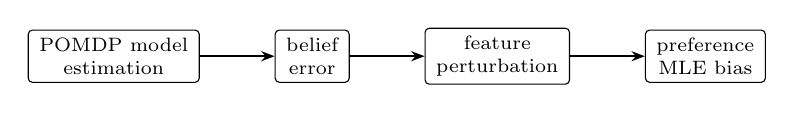
\begin{tikzpicture}[
  font=\scriptsize,
  node distance=0.95cm,
  box/.style={draw, rounded corners=1.5pt, inner xsep=4pt, inner ysep=3pt, align=center},
  arr/.style={-{Stealth[length=1.7mm]}, semithick}
]
\node[box] (est) {POMDP model\\ estimation};
\node[box, right=of est] (bel) {belief\\ error};
\node[box, right=of bel] (feat) {feature\\ perturbation};
\node[box, right=of feat] (mle) {preference\\ MLE bias};

\draw[arr] (est) -- (bel);
\draw[arr] (bel) -- (feat);
\draw[arr] (feat) -- (mle);
\end{tikzpicture}%
}
\caption{Error-propagation pipeline}
\label{fig:error-propagation-pipeline}
\vspace{-0.6em}
\end{figure}

The central technical obstacle is that Bayesian filtering is generally \emph{not} contractive in total variation and may amplify errors over time; stability requires conditions that jointly control transition mixing and informativeness of the observation channel. Building on a recent stochastic filter stability theorem \cite{Mcdonald2024StochasticCriteria}, we establish expectation-level stability and quantify the bias introduced by parametric model mismatch at each filtering step. This analysis yields an explicit Lipschitz stability bound for the parameter-to-belief mapping, along with high-probability control over the time-averaged belief error using a martingale argument. We first develop this mechanism for finite log-linear POMDPs and then extend it to neural-softmax POMDP models in the kernel regime, where finite-width linearization errors enter additively into the belief perturbation bound. These results can then be extended to define a uniform belief-accuracy event applicable across all comparisons within an RLHF dataset.

We position our analysis at the interface of controlled filter stability and preference-based reward estimation, to quantify how learned-dynamics error in a POMDP propagates through belief updates into reward learning in the belief-MDP. This belief mismatch perturbs the trajectory-level feature differences used in preference comparisons and the associated empirical feature covariance. We propagate these perturbations through a Bradley--Terry MLE analysis, obtaining a finite-sample reward recovery bound that separates (i) a statistical term vanishing with the number of human comparisons $N_{\mathrm{HF}}$, (ii) an irreducible model-mismatch bias controlled by filtering stability, and (iii) the regularization bias introduced to ensure well-posedness when the feature covariance is ill-conditioned or singular. This decomposition clarifies when preference-based RLHF remains statistically feasible under partial observability with an \emph{inexact} learned POMDP model, and which stability and modeling choices govern the achievable accuracy.

\paragraph{Contributions.}
\begin{itemize}[leftmargin=*]
\item \textbf{A theoretical framework for preference-based reward learning under partial observability.}
We establish, to the best of our knowledge, the first finite-sample reward-learning
guarantees for preference-based RLHF in POMDPs with inexact learned dynamics. We lift
the preference dataset into the belief-MDP representation and provide an explicit
error-propagation analysis from POMDP model mismatch to reward-estimation bias. This
setting is not covered by existing fully observed RLHF theory, where trajectory
features are assumed to be directly observed or exactly specified.

\item \textbf{Belief stability under learned log-linear and neural-softmax dynamics.}
We prove that the Bayesian belief filter is Lipschitz-stable in expectation under
parametric model error and a Dobrushin-type mixing condition
(Theorem~\ref{thm:param-belief-lip}). Unlike classical initialization-stability
results, model mismatch injects fresh error at every filtering step, requiring a
stronger sufficient contraction condition. We extend this mechanism to neural-softmax
models under a local NTK-style linearization event, where finite-width errors enter
additively. We then use martingale concentration to establish a uniform,
high-probability bound on time-averaged belief error across the dataset, yielding a
reusable belief-accuracy event.

\item \textbf{Robust Bradley--Terry reward learning from approximate beliefs.}
We derive a finite-sample guarantee for the constrained Bradley--Terry MLE
(Theorem~\ref{thm:main-mu}) that decomposes into a statistical error decaying as
$O(N_{\mathrm{HF}}^{-1/2})$, an irreducible model-mismatch bias controlled by belief
error, and a regularization bias. A key consequence is that, unlike in the fully
observed setting, more human feedback cannot reduce the estimation error below the
bias floor induced by imperfect dynamics, clarifying when and why reward learning
degrades under partial observability.


\end{itemize}




\paragraph{Organization.}
Section~\ref{sec:setup} introduces the POMDP model, log-linear dynamics, Bayesian filtering, and the induced belief-MDP representation.
Section~\ref{sec:belief-stability} derives expectation-level and high-probability stability guarantees for Bayesian filtering under learned log-linear dynamics. Appendix~\ref{sec:nn-extension} extends the belief-stability mechanism to neural-softmax models through an NTK-style linearization.
Section~\ref{sec:rlhf} formalizes the preference-learning setup and establishes our main reward estimation guarantee under belief approximation error.
Section~\ref{sec:conclusion} discusses implications, limitations, and future directions.
Technical proofs are deferred to the appendix.


%%%%%%%%%%%%%%%%%%%%%%%%%%%%%
%%%%%%%%%%%%%%%%%%%%%%%%%%%%%
\section{Related Work}
\label{sec:related_work}

Our setting draws on three adjacent literatures: learning under partial observability, stability of Bayesian filtering, and preference-based RLHF. POMDPs formalize decision-making with latent states and noisy observations \citep{Astrom1965}, but are statistically hard to learn in full generality \citep{Krishnamurthy2016, Jin2020}, motivating work under structural assumptions and algorithmic frameworks for planning and learning under partial observability \citep{KAELBLING199899, Du2019, liu2022sample, Golowich2022, Zhan2022, cayci2024recurrent}.

A closely related technical thread studies \emph{filter stability} under initialization error or model mismatch: classical analyses typically require strong mixing assumptions \citep{VanHandel2008}, while recent results provide explicit exponential stability via Dobrushin-type contractions that account for both transitions and observations \citep{Mcdonald2024StochasticCriteria}.

RLHF learns rewards from human feedback and then optimizes policies using standard RL machinery \citep{ChristianoLBMLA17, Wirth2017, Ji2023}. Reward learning is often instantiated via Bradley--Terry model \citep{Bradley1952, Plackett1975} and combined with policy optimization methods such as PPO \citep{Schulman2017}, underpinning successes in robotics and interactive systems \citep{Brown2019} and LLM alignment \citep{Ziegler2019, Stiennon2020, Bai2022, Ouyang2022, Achiam2023}. Recent theory analyzes preference-based MLE and RLHF-style learning in fully observed MDPs, from tabular regimes to function approximation and exploration-driven policy optimization \citep{Novoseller2020, Chen2022, ZhuPrincipledComparisons, Du2024Exploration-DrivenUtilization, kaufmann2025a, Saha2023}.

A smaller line of work connects RLHF to latent-state structure and non-Markovian rewards. Most closely, \citet{Kausik2024} model RLHF via \emph{partially-observed reward-states} (PORRL/PORMDP), where the environment state is observed but feedback depends on an additional latent ``internal'' reward-state. In contrast, we consider latent environment states with no access to rewards, and the agent interacts only through noisy observations and preference feedback. We quantify how belief computation under an \emph{inexact learned} dynamics model perturbs trajectory features and induces a principled bias in Bradley--Terry reward estimation.







%%%%%%%%%%%%%%%%%%%%%%%%%%%%%%%%%%%%%%%%%%%%%%%%%%%%%%%%%%%%%%%%%%%%%%%%%%%%
\section{Setup and Preliminaries}
\label{sec:setup}

\subsection{POMDP model and trajectories}
\label{subsec:pomdp}

We work with a finite POMDP \(
\bigl(\bS,\ \bA,\ \hat\bS,\ P_\theta,\ \Phi_w,\ r,\ \nu_0\bigr),
\) where \(\bS\) is the finite latent state space, \(\hat\bS\) is the finite observation space, \(\bA\) is the finite action set, \(P_\theta(\cdot\mid s,a)\in\Delta_{\bS}\) is the transition kernel, and \(\Phi_w(\cdot\mid s)\in\Delta_{\hat\bS}\) is the observation model. The reward function is \(r:\bS\times\bA\to\bR\), and the initial state distribution \(\nu_0\in\Delta_{\bS}\) is assumed known. The stability analysis below depends on the transition and observation channels only through their Dobrushin coefficients and the resulting explicit cardinality-dependent constants.

\begin{assumption}[Model structure and bounded features]\label{as:Model-LogLinear}

Model dynamics admit the following log-linear structure
\begin{align}
&P_\theta(s'|s,a)
=\frac{\exp\{\theta^\top\phi_p(s,a,s')\}}{\sum_{\bar s\in\bS}\exp\{\theta^\top\phi_p(s,a,\bar s)\}},\qquad
&
\Phi_{w}(\hat s\,|\,s)=\frac{\exp\{ w^\top \phi_\Phi(s,\hat s)\}}{\sum_{\bar s\in\hat \bS}\exp\{ w^\top\phi_\Phi(s,\bar s)\}}.\notag
\end{align}
\medskip\noindent
Here $\phi_p$ is a feature map for the transition kernel and $\phi_\Phi$ is a feature map for the observation model, and we assume
\[
\sup_{s,a,s'}\|\phi_p(s,a,s')\|_2\le B,\qquad
\sup_{s,\hat s}\|\phi_\Phi(s,\hat s)\|_2\le B.
\]
For some $B<\infty$. The initialization also satisfies
\begin{equation}\label{eq:mu-min-max}
1>\nu_{\max}\ge\nu_0(s)\ge\nu_{\min}>0, \qquad \forall s \in \bS. 
\end{equation}
\end{assumption}



\begin{remark}[Exponential-family modeling and model-based RL]\label{rem:expfam-mbrl}
The log-linear parametrizations in Assumption \ref{as:Model-LogLinear} are finite exponential-family models, standard in statistical modeling (e.g., \citet{bishop2007, wainwright2008, van2008hidden}). As a consequence, our framework falls under \emph{model-based RL}. One can use the assumed learned models for belief filtering and downstream policy optimization. In this work we focus on the preference-based reward learning guarantees, treating the policy-optimization stage as modular and leaving its integration to future work.
\end{remark}



% \begin{assumption}[Realizability and bounded parameter estimation error]\label{as:realizability-bounded-error}
% (Realizability) There exists a true parameter $\Theta^\star=(\theta^\star,w^\star)\in\bR^{d_\theta+d_w}$
% such that the data-generating POMDP uses transition kernel $P_{\theta^\star}$ and observation model $\Phi_{w^\star}$.
% \medskip
% \noindent
% (Bounded estimation error) Fix a radius $r_\Theta>0$ and assume the estimated parameter
% $\Theta=(\theta,w)$ satisfies
% \(\Theta \in \bB_2(\Theta^\star,r_\Theta)
% :=\bigl\{\Theta'\in\bR^{d_\theta+d_w}:\ \|\Theta'-\Theta^\star\|_2\le r_\Theta\bigr\}.
% \)
% Equivalently, \(\|\Theta-\Theta^\star\|_2^2=\|\theta-\theta^\star\|_2^2+\|w-w^\star\|_2^2 \le r_\Theta^2.\)
% We will use the shorthand
% \(\delta(\theta) := \|\theta-\theta^\star\|_2,\,\delta(w) := \|w-w^\star\|_2,
% \)
% so that $\delta(\theta)^2+\delta(w)^2\le r_\Theta^2$.
% \end{assumption}

\begin{assumption}[Realizability and local parameter error]\label{as:realizability-bounded-error}
There exists a true parameter \(\Theta^\star=(\theta^\star,w^\star)\in\mathbb{R}^{d_\theta+d_w}\)
such that the data-generating POMDP has transition kernel \(P_{\theta^\star}\) and observation model \(\Phi_{w^\star}\).

Fix \(r_\Theta>0\), and suppose the learned parameter \(\Theta=(\theta,w)\) satisfies
\[
\Theta \in \mathbb{B}_2(\Theta^\star,r_\Theta)
:= \{\Theta' \in \mathbb{R}^{d_\theta+d_w} : \|\Theta'-\Theta^\star\|_2 \le r_\Theta\}.
\]
Equivalently,
\[
\|\Theta-\Theta^\star\|_2^2
=
\|\theta-\theta^\star\|_2^2 + \|w-w^\star\|_2^2
\le r_\Theta^2.
\]
We write
\[
\delta(\theta):=\|\theta-\theta^\star\|_2,
\qquad
\delta(w):=\|w-w^\star\|_2,
\]
so that \(\delta(\theta)^2+\delta(w)^2\le r_\Theta^2\).
\end{assumption}

Given trajectories of observations and actions, a natural way to estimate the model parameter $\Theta=(\theta,w)$ in this class is via maximum-likelihood or an EM-type procedure. Fix a horizon $T\in\bN$. For a single trajectory, let the latent state sequence be
$Z := (s_{0:T})\in\bS^{T+1}$ and let the observation sequence be
$Y := (\hat s_{1:T},\, a_{0:T-1})\in \hat\bS^{T}\times\bA^{T}$.
We treat the action sequence $a_{0:T-1}$ as observed and work with the likelihood conditional on actions.
Under $\Theta=(\theta,w)$, the joint conditional trajectory likelihood factorizes as
\begin{align}\label{eq:traj-joint}
P_\Theta(Y,Z)
&=\nu_0(s_0)\,
\prod_{k=0}^{T-1} P_\theta(s_{k+1}\mid s_k,a_k)\,
\prod_{k=1}^{T}\Phi_w(\hat s_k\mid s_k).
\end{align}
Given a collection of trajectories, one may estimate $\Theta$ by maximizing the marginal likelihood $P_\Theta(Y)=\sum_Z P_\Theta(Y,Z),$ for example, via EM. Under standard local identifiability and regularity conditions (e.g., strong concavity/smoothness of the standard EM auxiliary objective, i.e., the expected complete-data log-likelihood in a neighborhood of $\Theta^\star$), EM-type procedures admit local linear convergence to $\Theta^\star$ at the population level, with corresponding finite-sample perturbation bounds \citep{HMMCappe, WANG20062001, van2008hidden, balakrishnan2017statistical}.




Given the observation--action history up to time $t$,
\(Y_t := (\hat s_{1:t},\, a_{0:t-1}),\) the corresponding belief is defined as
\[
b_t^\Theta(s)\;:=\;\bP_\Theta(s_t=s \mid Y_t)\in\Delta_{\bS},
\qquad b_0^\Theta(s)=\nu_0(s).
\]
For parameters $\Theta=(\theta,w)$, the Bayesian filter update is
\begin{align}\label{eq:belief-formula}
b_{t+1}^{\Theta}(s')
:=\frac{\Phi_w(\hat s_{t+1} \mid s')\sum_{s\in\bS}P_\theta(s'\mid s,a_t)\,b_t^{\Theta}(s)}
{\sum_{\bar s\in\bS}\Phi_w(\hat s_{t+1}\mid \bar s)\sum_{s\in\bS}P_\theta(\bar s\mid s,a_t)\,b_t^{\Theta}(s)}.
\end{align}
Moreover, the induced belief-MDP reward can be written as
\[
r_b(b_t^\Theta,a_t)
:=\bE_{s_t\sim b_t^\Theta}\!\big[r(s_t,a_t)\big]
=\sum_{s\in\bS} b_t^\Theta(s)\,r(s,a_t).
\]
The recursion Eq.~\ref{eq:belief-formula} defines a nonlinear operator on $\Delta_{\bS}$ obtained by composing a prediction step (via $P_\theta$) with a Bayes reweighting step (via $\Phi_w$). In general, this operator can amplify small perturbations in the model parameters or in the current belief over time. To obtain quantitative \emph{stability} guarantees for the belief process, we impose an explicit \emph{mixing} criterion that controls how strongly transitions forget the previous latent states. This is captured by the following Dobrushin coefficients, which will serve as the key constants governing one-step contraction and the resulting stability rate.

\medskip

\begin{definition}[Dobrushin coefficient]\label{def:dobrushin-controlled}
Let $P_\theta(\cdot\mid s,a)\in\Delta_{\bS}$ be the transition kernel and $\Phi_w\in\Delta_{\hat\bS}$ the observation model. Define the uniform Dobrushin coefficient of the models over the feasible choice of parameter set by

%$\bB_2(\theta^\star,r_\Theta)\times \bB_2(w^\star,r_\Theta)$, $s,s'\in\bS$ and $a\in \bA$

\[
\kappa_P:=\inf_{\theta}\inf_{s,s',a}
\sum_{x\in\bS}\min \{P_\theta(x\mid s,a),P_\theta(x\mid s',a)\},\qquad \kappa_\Phi := \inf_{w}\inf_{s,s'\in\bS}
\sum_{\hat s\in\hat\bS}\min\{\Phi_w(\hat s\mid s), \Phi_w(\hat{s}\mid s')\}.
\]

Equivalently, $$\kappa_P=1-\sup_{\theta}\sup_{a,s,s'}
\frac12\|P_\theta(\cdot\mid s,a)-P_\theta(\cdot\mid s',a)\|_1.$$
\end{definition}

 
\begin{assumption}[Dobrushin stability]\label{as:Dobrushin-stability}
Let \(\kappa_P,\kappa_\Phi\in(0,1]\) be the uniform Dobrushin coefficients in Definition~\ref{def:dobrushin-controlled}. Assume that
\[
\alpha := (1-\kappa_P)(4-3\kappa_\Phi) < 1.
\]
\end{assumption}

\begin{remark}[Role of \(\alpha\)]\label{rem:alpha-control}
In the log-linear model, Lemma~\ref{lem:Dobrushin-row-col} yields the explicit lower bounds
\[
\kappa_P\ge \frac{|\bS|}{1+(|\bS|-1)\exp\bigl(2B(\|\theta^\star\|_2+r_\Theta)\bigr)},\qquad
\kappa_\Phi\ge \frac{|\hat\bS|}{1+(|\hat\bS|-1)\exp\bigl(2B(\|w^\star\|_2+r_\Theta)\bigr)}.
\] Therefore, $\alpha$ can be controlled by the feature bound $B$ and the feasible radii; for example, by introducing temperature parameters to control the magnitude of $B$, one can effectively reduce $\alpha$. This condition is a non-trivial stability requirement since the Bayesian filtering update need not be a contraction in general (see Example 3.3, \cite{Mcdonald2024StochasticCriteria}). 

\paragraph{Practical note.}
Although $\kappa_P$ and $\kappa_\Phi$ are worst-case quantities, in practice rather than plugging in analytic lower bounds
Eq.~\ref{eq:dobrushin-row} and Eq.~\ref{eq:dobrushin-Phi} that must hold uniformly over all $(s,s',a)$ in the feasible parameter set, we can estimate $\kappa_P$ and $\kappa_\Phi$ directly from the realized transition and observation kernels. This yields a substantially less pessimistic stability certificate and better matches the observed contraction. 
 
To show exponential filter stability in expectation for an \emph{incorrectly initialized} POMDP, \citet{Mcdonald2024StochasticCriteria} assumed $(1-\kappa_P)(2-\kappa_\Phi)<1$. Building on this result, we show filter stability in expectation under POMDP model parameter perturbation. We set the assumption $(1-\kappa_P)(4-3\kappa_\Phi)<1$ in Theorem \ref{thm:param-belief-lip}. The stronger $(4-3\kappa_\Phi)$ factor arises because model mismatch injects fresh error at every step, as shown by terms (I)-(II) in Appendix \ref{proof-thm-belief}, and not just an initial discrepancy. This assumption is a \emph{sufficient} technical bridge from POMDP model-mismatch to robust preference-based reward learning, as formalized in Theorem \ref{thm:main-mu}. We emphasize that this assumption is not claimed to be a \emph{necessary} condition for the relation to hold; empirical performance may remain robust even when these worst-case mixing bounds are not strictly satisfied.
\end{remark}

\noindent
The next section quantifies this effect by proving that, under $\alpha<1$, the belief mapping $\Theta\mapsto b_t^\Theta$ is Lipschitz in expectation around $\Theta^\star$ (Theorem~\ref{thm:param-belief-lip}). This stability bound is the key technical input for transferring POMDP parameter error into controlled feature perturbations in the downstream RLHF analysis (Theorem~\ref{thm:main-mu}).
\medskip

%%%%%%%%%%%%%%%%%%%%%%%%%%%%%%%%%%%%%%%%%%%%%%%%%%%%%%%%%%%%%%%%%%%%%%%%%%%%
\section{Belief Stability Under Model Mismatch}
\label{sec:belief-stability}

Let the true parameters be \(\Theta^\star=(\theta^\star,w^\star)\) and the estimate
\(\Theta=(\theta,w)\), living in a compact feasible parameter set as in
Assumption~\ref{as:realizability-bounded-error}.

 
\label{subsec:belief-expectation}

\begin{theorem}\label{thm:param-belief-lip}
Consider the POMDP with log-linear dynamics, under Assumptions
\ref{as:Model-LogLinear}, \ref{as:realizability-bounded-error}, \ref{as:Dobrushin-stability}.
Fix an action sequence $(a_0,\dots,a_{t-1})$, estimated model parameters $\Theta=(\theta,w)$, true parameters $\Theta^\star=(\theta^\star,w^\star)$ and corresponding belief processes  $(b_k^\Theta)_{k=0}^t$ and $(b_k^{\Theta^\star})_{k=0}^t$ with priors $b_0^\Theta=b_0^{\Theta^\star}=\nu_0\in\Delta_{\bS}$.
Then, the mapping from parameters $\Theta =(\theta, w)\to b_t^\Theta$ is Lipschitz at $\Theta^\star$ in expectation. In particular, for every $t\ge1$,
\begin{align}\label{eq:belief-lipschitz}
\bE\Big[\|b_{t}^\Theta-b_{t}^{\Theta^\star}\|_{\mathrm{TV}}\Big]
\le \frac{(1-\alpha^{t})}{1-\alpha}c_b\,(\delta(\theta),\delta(w)),
\end{align}
where $c_b\, (\delta(\theta),\delta(w)):=B\bigl(\,\delta(w)+\frac{(3-2\kappa_\Phi)}{2}\,\delta(\theta)\bigr),$ and the expectation is over $\hat s_{1:t}\sim P_{\Theta^\star}(\,\cdot\,|a_{0:t-1}).$
\end{theorem}

\paragraph{Proof sketch.}
The proof decomposes one-step belief error into (I) observation-model perturbation, (II) transition-model perturbation, and (III) propagation under filter mixing, then unrolls the resulting recursion. The detailed proof is provided in Appendix \ref{proof-thm-belief}.

\begin{proof}
The full proof is given in Appendix \ref{proof-thm-belief}.
\end{proof}

\begin{remark}[Error in belief stability]\label{rem:belief-error-decomp}
The bound in Eq.~\ref{eq:belief-lipschitz} splits into a \emph{time-propagation} factor and a
\emph{one-step mismatch} term:
\begin{align*}
\bE\!\left[\|b_t^\Theta-b_t^{\Theta^\star}\|_{\mathrm{TV}}\right]
\;\le\;\underbrace{\frac{1-\alpha^t}{1-\alpha}}_{\text{propagation over time}}
\;\times\;\underbrace{\Big(B\,\delta(w)+\tfrac{B}{2}(3-2\kappa_\Phi)\,\delta(\theta)\Big)}_{\text{model mismatch}}.
\end{align*}

When $\alpha<1$, the propagation factor is uniformly bounded by $(1-\alpha)^{-1}$, so the
belief error scales linearly with the parameter deviations $\delta(w)$ and $\delta(\theta)$.
\end{remark}
\noindent




\begin{remark}[Filter stability challenges]
\label{rem:stability-context}
Analyzing filter stability over long horizons is notoriously difficult because the Bayesian update operator $\psi$ is generally \emph{not} a contraction and can expand the total variation distance between beliefs (see \citet{Mcdonald2024StochasticCriteria}, Example 3.3). Standard results often impose restrictive strong mixing conditions on the transition kernel $P(\cdot|\cdot,\cdot)$ and assume that it is sufficiently ergodic \cite{VanHandel2008}. Using the Dobrushin coefficient $\kappa_\Phi$ of the observation model can account for the \emph{joint} contraction properties of the transition and measurement steps, allowing for stability even when the transition kernel alone is not sufficiently mixing. The price for this generality is that the contraction holds in \emph{expectation} rather than almost surely. Moreover, while \citet{Mcdonald2024StochasticCriteria} establishes stability with respect to incorrect \emph{initialization}, our Theorem~\ref{thm:param-belief-lip} extends this machinery to the learning setting. We establish stability with respect to \emph{parametric model mismatch} ($\Theta$ vs.\ $\Theta^\star$), deriving explicit perturbation bounds specific to the log-linear family. This quantifies how parameter error injects bias at every step (terms (I) and (II) in Eq.~\ref{eq:belief-theorem-term-I} in Appendix \ref{proof-thm-belief}), a distinct challenge from the pure initialization decay studied in classical filtering literature.
\end{remark}



Theorem~\ref{thm:param-belief-lip} controls the belief error in \emph{expectation} at a fixed time $t$ under model mismatch. For the RLHF reduction we will need a \emph{uniform-in-time} control along a trajectory, since downstream feature and preference observations depend on the entire history. We therefore convert the per-step expected contraction into a \emph{high-probability bound} on the \emph{time-average} belief error.




\begin{definition}[Neural-softmax transition and observation models]
\label{def:nn-softmax-model}
Let the transition and observation kernels be parameterized by neural-network scores
\begin{align}\label{eq:nn-softmax-transition}
P_{W_p}(s' \mid s,a)
&=\frac{\exp\{F_p(s,a,s';W_p)\}}{\sum_{\bar s\in\bS}\exp\{F_p(s,a,\bar s;W_p)\}}\,\,,\qquad \Phi_{W_\Phi}(\hat s \mid s)=\frac{\exp\{F_\Phi(s,\hat s;W_\Phi)\}}
{\sum_{\bar s\in\hat\bS}\exp\{F_\Phi(s,\bar s;W_\Phi)\}}
\end{align}

We take both score functions to be two-layer ReLU networks with width \(m\). 
\end{definition}






\begin{corollary}[Belief perturbation bound for neural-softmax models]
\label{cor:nn-param-belief-lip}
Consider the POMDP introduced earlier with neural-softmax transition and observation models in Definition~\ref{def:nn-softmax-model}, under Assumption~\ref{as:nn-model-linearization}. Let \(W=(W_p,W_\Phi)\in\mathcal D\) be an estimated neural parameter and let \(W^\star=(W_p^\star,W_\Phi^\star)\in\mathcal D\) be the true parameter generating the POMDP. Consider an action sequence \((a_0,\dots,a_{t-1})\) and the corresponding belief processes \((b_k^W)_{k=0}^t\) and \((b_k^{W^\star})_{k=0}^t\), initialized from the same prior \(b_0^W=b_0^{W^\star}=\nu_0\in\Delta_{\bS}\). Let \(\kappa_P^{\mathrm{NN}}\) and \(\kappa_\Phi^{\mathrm{NN}}\) be the uniform neural Dobrushin coefficients from Lemma~\ref{lem:nn-Dobrushin-row-col}, and assume
\(
\alpha_{\mathrm{NN}}:=(1-\kappa_P^{\mathrm{NN}})(4-3\kappa_\Phi^{\mathrm{NN}})<1.
\)
For any \(\delta_{\mathrm{NN}}\in(0,1)\), on the event $\mathcal E_{\mathrm{lin}}^{\mathrm{NN}}(\delta_{\mathrm{NN}})$, and for every \(t\ge1\) it holds
\begin{align}\label{eq:nn-belief-lipschitz}
\bE\Big[\|b_t^W-b_t^{W^\star}\|_{\mathrm{TV}}\Big]
\le\frac{1-\alpha_{\mathrm{NN}}^t}{1-\alpha_{\mathrm{NN}}}\,
c_b^{\mathrm{NN}}(W,W^\star;\delta_{\mathrm{NN}}),
\end{align}
where the expectation is taken with respect to \(\hat s_{1:t}\sim P_{W^\star}(\,\cdot\,|a_{0:t-1})\), and
\begin{align}\label{eq:cb-nn-def}
c_b^{\mathrm{NN}}(W,W^\star;\delta_{\mathrm{NN}})
&:=B^{\mathrm{NN}}\|W_\Phi-W_\Phi^\star\|_F
+2\varepsilon_\Phi^{\mathrm{NN}}(m,\,\delta_{\mathrm{NN}})\\
&\qquad\qquad+(3-2\kappa_\Phi^{\mathrm{NN}})
\left(\frac{B^{\mathrm{NN}}}{2}\|W_p-W_p^\star\|_F
+\varepsilon_{p}^{\mathrm{NN}}(m,\,\delta_{\mathrm{NN}})\right).
\end{align}
In particular, as \(m\to\infty\), this recovers a Lipschitz-type belief perturbation bound in the neural parameters.
\end{corollary}

\begin{proof}
The full proof is given in Appendix \ref{proof:belief-lip-nn}.
\end{proof}

\paragraph{Proof sketch.}
The proof follows the same one-step decomposition as Theorem~\ref{thm:param-belief-lip}. The only changes are that the log-linear row-wise kernel perturbation bounds are replaced by Lemma~\ref{lem:nn-kernel-lip}, and the Dobrushin constants are replaced by the neural constants \(\kappa_P^{\mathrm{NN}}\) and \(\kappa_\Phi^{\mathrm{NN}}\) from Lemma~\ref{lem:nn-Dobrushin-row-col}. The resulting recursion has additive term \(c_b^{\mathrm{NN}}(W,W^\star;\delta_{\mathrm{NN}})\) and contraction coefficient \(\alpha_{\mathrm{NN}}\).



\subsection{High-probability time-average belief error}
\label{subsec:belief-highprob}

The expectation bounds in Theorems~\ref{thm:param-belief-lip} and Corollary ~\ref{cor:nn-param-belief-lip} control the belief mismatch at each fixed time. For preference-based reward learning, however, the relevant objects are trajectory-level feature sums, and hence the error
depends on the accumulated belief mismatch along the whole rollout. Therefore, it suffices to control the \emph{time-average} belief error. The following corollary converts the one-step
stability recursion into a high-probability time-average bound via a martingale
argument. This bound will later be union-bounded over all trajectory pairs in the
preference dataset to define a belief-accuracy event for the reward learning analysis.



\begin{corollary}\label{cor:belief-good-condition-cor}
Consider the setting of Theorem \ref{thm:param-belief-lip} and fix $\Theta=(\theta,w)\in\bB_2(\Theta^\star,r_\Theta)$ such that $\|\theta-\theta^\star\|_2\le\delta(\theta)$ and $\|w-w^\star\|_2\le\delta(w)$. For $t=0,1,\dots,T-1$ consider the random variables
\(
X_t :=\bigl\|b_t^\Theta-b_t^{\Theta^\star}\bigr\|_{\mathrm{TV}}.\) For the filtrations $\{\mathcal F_t^-\}_{t\ge 0}$ and $\{\mathcal F_t\}_{t\ge 0}$ defined by
\(
\mathcal F_t^- := \sigma(\hat s_{1:t},a_{0:t-1}),\mathcal F_t := \sigma(\hat s_{1:t},a_{0:t}),
\)
with $\mathcal F_{-1}^-:=\sigma(\varnothing,\Omega)$, the random variable $X_t$ is $\mathcal F_t^-$-measurable.  For any $\delta_b\in(0,1)$, with probability at least $1-\delta_b$,

\begin{align}\label{eq:hp-belief-freedman}
\frac{1}{T}\sum_{t=0}^{T-1}X_t &\le \frac{2c_b\,(\delta(\theta),\delta(w))}{1-\alpha} + \frac{2}{1-\alpha}\sqrt{\frac{2 c_b\,(\delta(\theta),\delta(w)) \log(1/\delta_b)}{T}}\notag\\
&\qquad\qquad+ \frac{\log(1/\delta_b)}{T(1-\alpha)}\left(\frac{4}{3} + \frac{2\alpha}{1-\alpha}\right)\\ &=: \epsilon_b(\delta_b).
\end{align}


Moreover, the same statement holds for the neural-softmax model of
Theorem~\ref{cor:nn-param-belief-lip}. In particular, for any
\(\delta_{\mathrm{NN}}\in(0,1)\), on the linearization event
\(\mathcal E_{\mathrm{lin}}^{\mathrm{NN}}(\delta_{\mathrm{NN}})\) from
Definition~\ref{def:nn-linearized-scores}, if \(
X_t^{\mathrm{NN}}:=\bigl\|b_t^W-b_t^{W^\star}\bigr\|_{\mathrm{TV}},
\) and if \(\alpha_{\mathrm{NN}}<1\), then with conditional probability at least \(1-\delta_b\), equivalently with joint probability at least \(1-(\delta_b+\delta_{\mathrm{NN}})\),

\begin{align}\label{eq:hp-belief-freedman-nn}
\frac{1}{T}\sum_{t=0}^{T-1}X_t^{\mathrm{NN}}
&\le \frac{2c_b^{\mathrm{NN}}(W,W^\star;\delta_{\mathrm{NN}})}{1-\alpha_{\mathrm{NN}}} +\frac{2}{1-\alpha_{\mathrm{NN}}}\sqrt{
\frac{2c_b^{\mathrm{NN}}(W,W^\star;\delta_{\mathrm{NN}})\log(1/\delta_b)}{T}}
\notag\\
&\qquad\qquad+\frac{\log(1/\delta_b)}{T(1-\alpha_{\mathrm{NN}})}
\left(\frac{4}{3} +\frac{2\alpha_{\mathrm{NN}}}{1-\alpha_{\mathrm{NN}}}\right)\\
&=:\epsilon_b^{\mathrm{NN}}(\delta_b,\delta_{\mathrm{NN}}),
\end{align}
where \(c_b^{\mathrm{NN}}(W,W^\star;\delta_{\mathrm{NN}})\) is defined in Eq.~\ref{eq:cb-nn-def}.
\end{corollary}



\paragraph{Proof sketch.}
Starting from a one-step conditional drift inequality for $X_t$, define a martingale difference sequence and apply Freedman’s inequality to control deviations of $\sum_t X_t$ from its conditional expectation, yielding the stated time-average bound.

\medskip

\begin{remark}[Learning Beliefs Directly]\label{rem:alternative-belief-approx}
Our analysis is modular with respect to the source of the approximate beliefs. 
Although Sections~\ref{sec:setup}--\ref{sec:belief-stability} instantiate $\tilde b_t=b_t^\Theta$ through Bayesian filtering under a learned POMDP model, one may instead use a direct belief-inference module that maps histories $(\hat s_{1:t},a_{0:t-1})$ to approximate beliefs. Recent examples include Deep Belief Markov Models \cite{DBeliefNN}, which learn belief-transition and belief-inference operators via variational inference, and flow-based recurrent belief models, which use normalizing flows to represent flexible belief distributions \citep{flowBelief}. This provides an alternative approach to bypass explicit POMDP model estimation when convenient. In our reward-learning analysis in the following section, such a module can be substituted for the Bayesian filter whenever it provides a belief-accuracy guarantee of the form
\[
\frac1T\sum_{t=0}^{T-1}\|\tilde b_t-b_t^{\Theta^\star}\|_{\mathrm{TV}}\le \epsilon_b^{\mathrm{approx}} .
\]
 
for some approximation error $\epsilon_b^{\mathrm{approx}}$. Then the belief-approximation error enters the next section only through the trajectory-feature perturbation term, and we can replace
$\epsilon_b(\delta_b,2N_{\mathrm{HF}})$ by $\epsilon_b^{\mathrm{approx}}$
to obtain the same bound on accumulated feature difference $\|\tilde\phi_i-\phi_i\|_2$, and the subsequent Bradley--Terry estimation analysis proceeds unchanged with this substituted error level.
\end{remark}


%%%%%%%%%%%%%%%%%%%%%%%%%%%%%%%%%%%%%%%%%%%%%%%%%%%%%%%%%%%%%%%%%%%%%%%%%%%%
\section{Preference-Based Reward Learning Under Belief Error}
\label{sec:rlhf}

\noindent
Having established quantitative belief stability under model mismatch, we turn to learning a reward model from pairwise preferences when trajectories are represented in the belief-MDP. Note that the model mismatch affects reward learning through the induced belief features, since preference labels come from rollouts, but the learner’s feature construction relies on $b_t^\Theta$ rather than the oracle beliefs $b_t^{\Theta^\star}$. Accordingly, this section formalizes the Bradley--Terry preference model \citep{Bradley1952, Wirth2017} over belief-based trajectory features, and quantifies how the belief error bounds from Section~\ref{sec:belief-stability} translate into an explicit perturbation (bias) term in reward estimation, alongside the usual finite-sample statistical error.


\subsection{Reward model and preference data}
\label{subsec:reward-pref-model}

\begin{assumption}[Reward model structure and preference data for belief-MDP]\label{assum:reward-rlhf}
\leavevmode
\begin{enumerate}
\item \textbf{Linear latent reward.}
For all $(s,a)\in\bS\times\bA$, the reward is linear:
\(r(s,a)=\phi_r(s,a)^\top \mu^\star\) with the corresponding feature map satisfying \(\|\phi_r(s,a)\|_2\le B_r < \infty\),
and the unknown reward parameter $\mu^\star\in\bB_2(r_\mu)\subset\bR^{d}$.

\item \textbf{Belief feature map.}
Define
\(\phi_b(b,a):=\sum_{s\in\bS}b(s)\,\phi_r(s,a)\) for \((b,a)\in\Delta_{\bS}\times\bA\).
Then \(r_b(b,a) :=\bE_{s\sim b}\big[r(s,a)\big]
=\sum_{s\in\bS} b(s)\,\phi_r(s,a)^\top\mu^\star
=\phi_b(b,a)^\top\mu^\star.\)
 

\item \textbf{Preference realizability.}
Let $\{(\tau_i^{(1)},\tau_i^{(2)},y_i)\}_{i=1}^{N_{\mathrm{HF}}}$ be $N_{\mathrm{HF}}$ independent preference comparisons with fixed trajectory horizon $T\in\bN$. Here $y_i\in\{0,1\}$ and $\sigma(z)=1/(1+e^{-z})$. Let $\phi_i\in\bR^{d}$ be the clean trajectory-level feature difference defined in Eq.~\ref{eq:accu-feature-exact}. Then, for every $i$,
\(\bP(y_i=1\mid \phi_i)=\sigma(\phi_i^\top\mu^\star).\)
\end{enumerate}
\end{assumption}


\begin{remark}
Since $\phi_b$ is linear in $b$, it inherits boundedness:
\[
\|\phi_b(b,a)\|_2 \le \sum_{s\in\bS} b(s)\,\|\phi_r(s,a)\|_2 \le B_r, \forall (b,a)\in\Delta_{\bS}\times\bA.
\]
Moreover, for any $b,b'\in\Delta_{\bS}$ and all $a\in\bA$,
\begin{align}\label{eq:belief-feature-lip}
\|\phi_b(b,a)&-\phi_b(b',a)\|_2
=\Big\|\sum_{s\in\bS}\big(b(s)-b'(s)\big)\phi_r(s,a)\Big\|_2\notag\\
&\le B_r\|b-b'\|_1
=2B_r\|b-b'\|_{\mathrm{TV}}.
\end{align}
\end{remark}

\begin{remark}[Generalization to non-linear rewards]
Linear reward parameterizations are standard in preference-based RLHF and are widely used as a tractable baseline (see, e.g., \cite{ZhuPrincipledComparisons, Du2024Exploration-DrivenUtilization, cen2025valueincentivized}). 
Our analysis isolates how model-mismatch propagates through belief errors into perturbed trajectory features, which in turn affects reward learning in Theorem \ref{thm:main-mu}. 
More general reward function classes can be accommodated by introducing an approximation error term (relative to the linear class) and carrying it through the final bound. 
In particular, over-parameterized neural networks are a plausible choice as discussed in Appendix ~\ref{sec:nn-extension} for POMDP model approximation.
\end{remark}
 
\subsection{Clean vs.\ perturbed trajectory features and MLE}
\label{subsec:features-mle}

Throughout the following, we work on the belief state space $\Delta_{\bS}$ and use the belief feature map
$\phi_b$. Let $N_{\mathrm{HF}}$ denote the number of \emph{independent} preference comparisons, and consider a dataset
\(
\bigl\{(\tau_i^{(1)},\tau_i^{(2)},y_i)\bigr\}_{i=1}^{N_{\mathrm{HF}}}
\),
where $y_i\in\{0,1\}$ is the observed preference label and $y_i=1$ indicates a preference for $\tau_i^{(1)}$ over $\tau_i^{(2)}$. For each $i\in\{1,\dots,N_{\mathrm{HF}}\}$ and $j\in\{1,2\}$, let the observed history be \(Y_i^{(j)} \;:=\; \bigl(\hat s_{i,1:T}^{(j)},\,a_{i,0:T-1}^{(j)}\bigr).
\) and define the corresponding belief sequences $(b_{i,h}^{(j),\Theta})_{h=0}^{T-1}$ and
$(b_{i,h}^{(j),\Theta^\star})_{h=0}^{T-1}$ as the filtering distributions computed under
$\Theta$ and $\Theta^\star$, respectively, on the \emph{same} history $Y_i^{(j)}$ via the Bayesian update
Eq.~\ref{eq:belief-formula}. We then write the history-indexed belief trajectories as
\(
\tau_i^{(j),\Theta}:=\bigl(b_{i,h}^{(j),\Theta},\,a_{i,h}^{(j)}\bigr)_{h=0}^{T-1}, \tau_i^{(j),\Theta^\star}:=\bigl(b_{i,h}^{(j),\Theta^\star},\,a_{i,h}^{(j)}\bigr)_{h=0}^{T-1}
\), and the action sequence $(a_{i,h}^{(j)})_{h=0}^{T-1}$ is treated as observed. Throughout this work, we assume that all trajectories have a fixed horizon $T<\infty$.


 \begin{remark}[Single realized action sequence vs.\ fixed-history analysis]\label{rem:one-action-seq}
In an RLHF interaction there is only one physically realized history $(\hat s_{1:T},a_{0:T-1})$.
Our stability guarantees compare $b_t^\Theta$ and $b_t^{\Theta^\star}$ computed on this \emph{same realized history}
(i.e., conditioning on the realized action sequence and coupling on the realized observations).
This fixed-history coupling is exactly what controls feature perturbations in Eq.~\ref{eq:accu-feature-exact}--Eq.~\ref{eq:accu-feature-perturbed}.
Analyzing additional divergence caused by two models inducing different closed-loop action sequences is beyond scope.
\end{remark}

  
\paragraph{Reward parameter learning from human preferences.}
We consider the estimation of the reward parameter $\mu^\star\in\bR^d$ from human preference data under a trajectory-level Bradley--Terry model \cite{Bradley1952}. Human feedback is provided as pairwise trajectory comparisons $\{(\tau_i^{(1)},\tau_i^{(2)},y_i)\}_{i=1}^{N_{\mathrm{HF}}}$. For each comparison, we define the trajectory-level exact and perturbed accumulated feature differences as

\begin{equation}\label{eq:accu-feature-exact}
\phi_i:=\sum_{h=0}^{T-1}\phi_b \bigl(b_{i,h}^{(1),\Theta^\star},a_{i,h}^{(1)}\bigr)-\sum_{h=0}^{T-1}\phi_b \bigl(b_{i,h}^{(2),\Theta^\star},a_{i,h}^{(2)}\bigr),
\end{equation}
\begin{equation}\label{eq:accu-feature-perturbed}
\tilde\phi_i:=\sum_{h=0}^{T-1} \phi_b \bigl(b_{i,h}^{(1),\Theta}, a_{i,h}^{(1)}\bigr)
-\sum_{h=0}^{T-1} \phi_b \bigl(b_{i,h}^{(2),\Theta}, a_{i,h}^{(2)}\bigr).
\end{equation}
The feature vector $\phi_i$ corresponds to the trajectory-level reward feature difference evaluated along the true belief process $(b_{i,h}^{(j),\Theta^\star})_{h}$.
The perturbed feature $\tilde\phi_i$ is computed using approximate beliefs $(b_{i,h}^{(j),\Theta})_{h}$, where the differences arise from model mismatch. Lemma \ref{lem:Delta-Bound} bounds  $\|\phi_i-\tilde\phi_i\|_2$ on the event $\mathcal E_{b}^{\mathrm{RLHF}}(\delta_b)$ in the Appendix. These two features induce conditional preference models; for example,
\(
\tilde\phi_i
\)
induces
\(
\bP(y_i=1\mid \tilde\phi_i,\mu)=\sigma(\tilde\phi_i^\top\mu)
\),
with $\sigma(z)=1/(1+e^{-z})$.
We estimate the reward parameter using the constrained maximum likelihood estimator
\begin{align}\label{eq:reward-mle}
\tilde\mu\;&:=\;\argmin_{\|\mu\|_2\le r_\mu}\Bigg\{-\sum_{i=1}^{N_{\mathrm{HF}}}\Big[y_i\log\sigma(\tilde\phi_i^\top\mu)
+(1-y_i)\log \bigl(1-\sigma(\tilde\phi_i^\top\mu)\bigr)\Big]\Bigg\}.
\end{align}
In the following analysis, we study the statistical behavior of $\tilde\mu$ and its robustness to trajectory-level perturbations arising from belief approximation. For clarity, the complete computational pipeline from recursive belief filtering to the optimization of the regularized estimator in Eq.~\ref{eq:reward-mle} is summarized in Algorithm \ref{alg:reward-learning}.

\begin{remark}[Belief-based features]
Classical Bradley--Terry reward learning typically assumes access to true states and uses state-based trajectory features \citep{Wirth2017, ZhuPrincipledComparisons, Du2019, cen2025valueincentivized}. Under partial observability, we instead construct $\phi_i$ and $\tilde\phi_i$ from belief--action pairs; hence model mismatch affects reward learning through belief-induced feature perturbations.
\end{remark}


\begin{algorithm}[t]
\caption{Preference-Based Reward Learning via Learned Beliefs}
\label{alg:reward-learning}
\begin{algorithmic}[1]
\STATE \textbf{Input:}
Horizon $T$;
preference data $\mathcal{D} = \{(Y_i^{(1)},Y_i^{(2)},y_i)\}_{i=1}^{N_{\mathrm{HF}}}$ with
$Y_i^{(j)}=(\hat s^{(j)}_{i,1:T},a^{(j)}_{i,0:T-1})$;
labels $y_i\in\{0,1\}$;
learned POMDP model $\Theta=(\theta,w)$; belief feature map $\phi_b$; constraint radius $r_\mu$.

\STATE \textit{Phase 1: Reconstruct Beliefs and Features}
\FOR{$i=1,\dots,N_{\mathrm{HF}}$}
    \FOR{$j\in\{1,2\}$}
        \STATE $b^{(j),\Theta}_{i,0}\gets \nu_0$
        \FOR{$h=0,\dots,T-1$}
            \STATE $b^{(j),\Theta}_{i,h+1}\gets \text{BeliefUpdate}\!\left(
            b^{(j),\Theta}_{i,h},a^{(j)}_{i,h},\hat s^{(j)}_{i,h+1};\Theta\right)$
            \hfill{\small (Eq.~\ref{eq:belief-formula})}
        \ENDFOR
    \ENDFOR
    \STATE Compute perturbed feature difference $\tilde\phi_i$ (Eq.~\ref{eq:accu-feature-perturbed}):
    \STATE $\tilde\phi_i \gets \sum_{h=0}^{T-1}\phi_b\!\left(b^{(1),\Theta}_{i,h},a^{(1)}_{i,h}\right)
                 \;-\; \sum_{h=0}^{T-1}\phi_b\!\left(b^{(2),\Theta}_{i,h},a^{(2)}_{i,h}\right)$
\ENDFOR

\STATE \textit{Phase 2: Maximum Likelihood Estimation}
\STATE Solve for $\tilde\mu$ (Eq.~\ref{eq:reward-mle}):
\STATE $\tilde\mu \gets \argmin_{\|\mu\|_2\le r_\mu}\;
-\sum_{i=1}^{N_{\mathrm{HF}}}\Big[y_i\log\sigma(\tilde\phi_i^\top\mu)
+(1-y_i)\log\big(1-\sigma(\tilde\phi_i^\top\mu)\big)\Big]$

\STATE \textbf{Output:} Estimated reward parameter $\tilde\mu$
\end{algorithmic}
\end{algorithm}





%%%%%%%%%%%%%%%%%%%%%%%%%%%%%%%%
%%%%%%%%%%%%%%%%%%%%%%%%%%%%%
%==========================
\subsection{Belief accuracy event for preference learning}
\label{subsec:belief-event}
In this subsection we lift the time-average belief error guarantee from
Corollary~\ref{cor:belief-good-condition-cor} to the full preference dataset.
Note that we do \emph{not} need a uniform-in-time control such as
$\sup_{0\le h\le T-1}\|b_h^\Theta-b_h^{\Theta^\star}\|_{\mathrm{TV}}$.
Since Bradley--Terry comparisons are driven by accumulated trajectory-level  feature differences (\ref{eq:accu-feature-exact} and \ref{eq:accu-feature-perturbed}), the relevant quantity is the \emph{per-trajectory time-average} belief
mismatch, which then translates into a bound on the induced feature perturbation.
We therefore define a high-probability event on which every rollout used to form the
comparisons satisfies a small average belief error.

\textbf{Belief accuracy event.}
Consider preference comparisons $\{(\tau_i^{(1)},\tau_i^{(2)},y_i)\}_{i=1}^{N_{\mathrm{HF}}}$. For any confidence level $\delta_b\in(0,1)$, define the belief-accuracy events for $i\in\{1,\dots,N_{\mathrm{HF}}\},\ j\in\{1,2\}$ as
\begin{equation}\label{eq:Eb-RLHF-uniform}
\mathcal E_{b,i}^{(j)}(\delta_b)\;:=\;\left\{\frac{1}{T}\sum_{h=0}^{T-1}
\bigl\|b_{i,h}^{(j),\Theta}-b_{i,h}^{(j),\Theta^\star}\bigr\|_{\mathrm{TV}}
\ \le\ \epsilon_b(\delta_b)\right\},\quad \mathcal E_{b}^{\mathrm{RLHF}}(\delta_b)\;:=\;\bigcap_{i=1}^{N_{\mathrm{HF}}}\ \bigcap_{j\in\{1,2\}}
\mathcal E_{b,i}^{(j)} \left(\frac{\delta_b}{2N_{\mathrm{HF}}}\right).
\end{equation}
By Corollary~\ref{cor:belief-good-condition-cor} and a union bound,
\(
\bP\bigl(\mathcal E_{b}^{\mathrm{RLHF}}(\delta_b)\bigr)\ \ge\ 1-\delta_b.
\)
Throughout the following analysis, we work on the event $\mathcal E_{b}^{\mathrm{RLHF}}(\delta_b)$ for log-linear POMDP model and use the shorthand
\begin{align}\label{eq:eps-b-bar-def}
\epsilon_b(\delta_b, 2N_{\mathrm{HF}}):=\;\epsilon_b \left(\frac{\delta_b}{2N_{\mathrm{HF}}}\right)&=\frac{2c_b\,(\delta(\theta),\delta(w))}{1-\alpha}+ \frac{2}{1-\alpha}\sqrt{\frac{2 c_b\,(\delta(\theta),\delta(w)) \log(2N_{\mathrm{HF}}/\delta_b)}{T}}\notag\\[6pt]
&\qquad\qquad+\frac{\log(2N_{\mathrm{HF}}/\delta_b)}{T(1-\alpha)}\left(\frac{4}{3}+ \frac{2\alpha}{1-\alpha}\right).
\end{align}
That is, $\epsilon_b(\delta_b, 2N_{\mathrm{HF}})$ is given by Eq.~\ref{eq:hp-belief-freedman} with the substitution
$\log\bigl(2N_{\mathrm{HF}}/\delta_b\bigr)$. Analogously, for the neural-softmax POMDP model under the setting of Theorem~\ref{cor:nn-param-belief-lip}, fix \(\delta_{\mathrm{NN}}\in(0,1)\). On the event \(\mathcal E_{\mathrm{lin}}^{\mathrm{NN}}(\delta_{\mathrm{NN}})\), define \(\mathcal E_{b}^{\mathrm{RLHF},\mathrm{NN}}(\delta_b,\delta_{\mathrm{NN}})\) similarly to Eq.~\ref{eq:Eb-RLHF-uniform}, with \(b_{i,h}^{(j),\Theta}\) and \(b_{i,h}^{(j),\Theta^\star}\) replaced by \(b_{i,h}^{(j),W}\) and \(b_{i,h}^{(j),W^\star}\), respectively, and with \(\epsilon_b\) replaced by the neural bound \(\epsilon_b^{\mathrm{NN}}\). More explicitly, we use the shorthand
\[
\epsilon_b^{\mathrm{NN}}(\delta_b,2N_{\mathrm{HF}},\delta_{\mathrm{NN}})
:=\epsilon_b^{\mathrm{NN}}\!\left(\frac{\delta_b}{2N_{\mathrm{HF}}},\delta_{\mathrm{NN}}\right),
\]
where \(\epsilon_b^{\mathrm{NN}}(\cdot,\delta_{\mathrm{NN}})\) is defined in Eq.~\ref{eq:hp-belief-freedman-nn} using the linearization-error levels
\(\varepsilon_p^{\mathrm{NN}}(m,\delta_{\mathrm{NN}})\) and
\(\varepsilon_\Phi^{\mathrm{NN}}(m,\delta_{\mathrm{NN}})\). By the neural high-probability belief bound and a union bound over the \(2N_{\mathrm{HF}}\) trajectories, together with \(\mathcal E_{\mathrm{lin}}^{\mathrm{NN}}(\delta_{\mathrm{NN}})\), we have
\[
\bP\!\left(\mathcal E_{b}^{\mathrm{RLHF},\mathrm{NN}}(\delta_b,\delta_{\mathrm{NN}})\right)
\ge 1-(\delta_b+\delta_{\mathrm{NN}}).
\]

\begin{remark}[Preference realizability and conditional independence]\label{remark:label-cond-indep}
Assumption~\ref{assum:reward-rlhf} (item~3) assumes a correctly specified Bradley--Terry preference model, where each label $y_i$ is generated from an independent trajectory pair and is conditionally independent given the corresponding clean feature difference $\phi_i$, with \(
\bP(y_i=1\mid \phi_i)=\sigma(\phi_i^\top\mu^\star).
\) This provides the link from trajectory-level features to observable preference feedback. (See, also Proof \ref{lem:clean-like-grad-bound})
\end{remark}


 \subsection{Reward estimation guarantee}\label{subsec:main-reward-thm}

 
We now state our main theorem for estimating the Bradley--Terry reward parameter
$\mu^\star$. Our analysis is carried out in the \emph{local geometry} induced by the
empirical design covariance, which captures the curvature of the empirical MLE objective. Accordingly, we measure error in the
covariance-weighted norm $\|\cdot\|_{\tilde\Sigma+\zeta I}$, (See Definition \ref{def:clean-pert-cov}), which is a natural
scale for evaluating the parameter optimality gap. However, our learner features are
\emph{perturbed} through belief mismatch, so the usual self-normalized arguments \cite{ZhuPrincipledComparisons, NIPS2011_e1d5be1c} cannot be applied directly to the gradient formed with $\tilde\phi_i$.
This introduces an additional technical difficulty; see Remark~\ref{remark:why-not-exact-cov}.

\begin{definition}[Clean and perturbed empirical covariances]\label{def:clean-pert-cov}
Given trajectory-level feature differences $\{\phi_i\}_{i=1}^{N_{\mathrm{HF}}}$ and their perturbed counterparts
$\{\tilde\phi_i\}_{i=1}^{N_{\mathrm{HF}}}$, define the corresponding empirical covariance matrices by
\begin{equation}\label{eq:sigma-cov-hf}
\Sigma \;:=\; \frac{1}{N_{\mathrm{HF}}}\sum_{i=1}^{N_{\mathrm{HF}}}\phi_i\phi_i^\top,
\qquad
\tilde\Sigma \;:=\; \frac{1}{N_{\mathrm{HF}}}\sum_{i=1}^{N_{\mathrm{HF}}}\tilde\phi_i\tilde\phi_i^\top.
\end{equation}
\end{definition}

\begin{theorem}[Reward parameter estimation under belief error]\label{thm:main-mu}
Assume the conditions of Theorem~\ref{thm:param-belief-lip} and Assumption \ref{assum:reward-rlhf}. Let $\Theta=(\theta,w)\in\bB_2(\Theta^\star,r_\Theta)$ and let
$\{(Y_i^{(1)},Y_i^{(2)},y_i)\}_{i=1}^{N_{\mathrm{HF}}}$ be $N_{\mathrm{HF}}$ independent preference comparisons. Form perturbed trajectory feature differences $\{\tilde\phi_i\}_{i=1}^{N_{\mathrm{HF}}}$ via Eq.~\ref{eq:accu-feature-perturbed}
using beliefs $(b_{i,h}^{(j),\Theta})_{h=0}^{T}$ computed from Eq.~\ref{eq:belief-formula}, and let
$\tilde\mu$ be the constrained Bradley--Terry MLE in Eq.~\ref{eq:reward-mle}.
Fix $\delta_b,\delta_c\in(0,1)$. Then, for any factor $c_{\zeta}>1$, with probability at least $1-(\delta_b+\delta_c)$,
the estimation error satisfies

\begin{align}
\|\tilde\mu-\mu^\star\|_{\tilde\Sigma+\zeta I}
\le &\frac{2\sqrt{c_{\zeta}}}{\rho\sqrt{N_{\mathrm{HF}}(c_{\zeta}-1)}}\sqrt{d\log \Big(1+\frac{4T^2 B_r^2}{\zeta d}\Big)+2\log \Big(\frac{1}{\delta_c}\Big)} \notag\\[8pt]
&\qquad\qquad+ \frac{8T B_r\,\epsilon_b(\delta_b, 2N_{\mathrm{HF}})}{\rho\sqrt{\zeta }}\, \Bigl(1+\tfrac12\,T B_r\,r_\mu\Bigr)+2r_\mu\sqrt{\zeta }\\
&:=\,\epsilon(\delta_b,\delta_c,\zeta),
\label{eq:main_mu_bound}
\end{align}
where $\rho\,=\;1/\big(2+\exp(2T B_r r_\mu)+\exp(-2T B_r r_\mu)\big)$, and $\zeta:=c_{\zeta} 16T^2B_r^2\epsilon_b(\delta_b, 2N_{\mathrm{HF}})(1+\epsilon_b(\delta_b, 2N_{\mathrm{HF}}))$.

The same conclusion holds for the neural-softmax POMDP model of
Theorem~\ref{cor:nn-param-belief-lip}. In that case, additionally fix \(\delta_{\mathrm{NN}}\in(0,1)\). With probability at least
\(1-(\delta_b+\delta_c+\delta_{\mathrm{NN}})\), the bound
Eq.~\ref{eq:main_mu_bound} holds after replacing
\(b_{i,h}^{(j),\Theta},b_{i,h}^{(j),\Theta^\star}\) by
\(b_{i,h}^{(j),W},b_{i,h}^{(j),W^\star}\), respectively, and replacing
\(\epsilon_b(\delta_b,2N_{\mathrm{HF}})\) everywhere, including in the definition of
\(\zeta\), by \(
\epsilon_b^{\mathrm{NN}}(\delta_b,2N_{\mathrm{HF}},\delta_{\mathrm{NN}}).
\)

\end{theorem}

\begin{proof}[Proof sketch]
We show $\tilde L$ is $\rho$-strongly convex on $\bB_2(r_\mu)$ in the $(\tilde\Sigma+\zeta I)$-geometry, and then control the estimation error by bounding the gradient at $\mu^\star$ \(
\|\tilde\mu-\mu^\star\|_{\tilde\Sigma+\zeta I} \;\le\; \frac{2}{\rho}\,\|\nabla \tilde L(\mu^\star)\|_{(\tilde\Sigma+\zeta I)^{-1}} \;+\;2r_\mu\sqrt{\zeta }\). Then, we decompose $\nabla \tilde L(\mu^\star)$ into (i) a clean term handled by an elliptical-potential bound, and (ii) a perturbation term controlled on $\mathcal E_b^{\mathrm{RLHF}}(\delta_b)$. Finally, we transfer the bound from the clean norm $(\Sigma+\zeta I)$ to the perturbed norm $(\tilde\Sigma+\zeta I)$ by an inverse-comparison argument. More details on $\zeta$ is provided in Remarks \ref{rem:zeta-explicit}-\ref{rem:zeta-choice}. The proof for neural-softmax POMDP is similar.
\end{proof}

\begin{proof}
The full proof is given in Appendix \ref{proof:thm-rlhf}.
\end{proof}


\begin{remark}[The cost of partial observability and error decomposition]
Compare Theorem~\ref{thm:main-mu} to the oracle fully observed setting, where the learner observes the true state and thus eliminats the belief-induced model-mismatch bias terms. In that case one recovers the standard $
\tilde O\!\left(\sqrt{\frac{d}{\rho^2 N_{\mathrm{HF}}}}\right)
$ decay rate (e.g., Lemma 5.1. \citet{ZhuPrincipledComparisons}).
In contrast, under partial observability with a fixed learned dynamics model, the bound contains additional terms that do not decay with $N_{\mathrm{HF}}$; hence letting $N_{\mathrm{HF}}\to\infty$ cannot reduce the reward-estimation error upper bound below this bias floor. This separates the benefit of more feedback from the price of operating with approximate beliefs. More precisely, the bound in Theorem~\ref{thm:main-mu} separates three contributions to the parameter error. Up to logarithmic factors,
\begin{align*}
    \|\tilde\mu-\mu^\star\|_{\tilde\Sigma+\zeta I}\;\;\lesssim\;\;\underbrace{\mathcal{O}\!\left(\frac{1}{\sqrt{N_{\mathrm{HF}}}}\right)}_{\text{ Statistical Noise}}+\underbrace{\mathcal{O}\!\left(\frac{T B_r}{\sqrt{\zeta}}\;\epsilon_b(\delta_b,2N_{\mathrm{HF}})\right)}_{\text{ Model-Mismatch Bias}}
    \;+\;\underbrace{\mathcal{O}(r_\mu\sqrt{\zeta})}_{\text{ Regularization Bias}}.
\end{align*}

\end{remark}

\section{Conclusion}
\label{sec:conclusion}
We analyzed preference-based reward learning in belief-MDPs under partial observability, where the true environment state is latent, and the agent instead acts on belief states obtained by Bayesian filtering from observation histories under an inexact learned POMDP. For finite log-linear POMDPs, we proved explicit stability of the filtering recursion to parametric model mismatch under a Dobrushin-type mixing condition, yielding bounds on $\bE[\|b_t^\Theta-b_t^{\Theta^\star}\|_{\mathrm{TV}}]$ and high-probability time-average control. We further extended the same belief-stability mechanism to neural-softmax POMDP models through an NTK-style linearization, where finite-width linearization errors enter additively into the belief perturbation bound. We then propagated belief mismatch into trajectory-level feature perturbations and derived finite-sample guarantees for Bradley--Terry reward estimation from preferences, decomposing the error upper bound into an $N_{\mathrm{HF}}^{-1/2}$ statistical term, an irreducible model-mismatch bias controlled by the belief error level, and a regularization bias governed by $\zeta$.

A limitation is that our filter comparison treats the action sequence as given and studies stability under a common logged action--observation history, which is the relevant regime for offline RLHF on a fixed dataset \cite{kaufmann2025a}. Also, the Dobrushin contraction assumption can be conservative in weakly mixing or nearly deterministic regimes and may only be valid in a local neighborhood of the true parameters. For the neural-softmax extension, the guarantee additionally relies on a lazy-training regime, so the resulting constants depend on the width-dependent approximation errors.

As future directions, one can consider end-to-end closed-loop guarantees that couple belief-filter error with policy-induced trajectory drift, develop weaker stability notions beyond uniform Dobrushin contraction, and extend the analysis to broader learned-dynamics function classes with explicit approximation terms. A natural complementary module is a POMDP parameter-estimation stage, for either log-linear or neural transition and observation models, with finite-sample error control, enabling a fully modular pipeline in which estimation, filtering stability, preference-based reward learning, and policy optimization in the continuous belief-MDP are analyzed and improved componentwise.




\newpage

%%%%%%%%%%%%%%%%%%%%%%%%%%%%%%%%%%%%%%%%%%%%%%%%%%%%%%%%%%%%%%%%%%%%%%%%%%%%
% \section{Implications and Design Guidance}
% \label{sec:implications}

% We summarize how the bounds depend on the key quantities already present in the statements.
% \paragraph{Effect of log-linear feature bound $B$.}
% The bound $B$ controls (i) the explicit Dobrushin lower bounds in Remark~\ref{rem:alpha-control} and (ii) the constant $c_b(\delta(\theta),\delta(w))$ in Theorem~\ref{thm:param-belief-lip}. In particular, a smaller $B$ improves the contraction constants and decreases $c_b(\delta(\theta),\delta(w))$.
% However, $B$ is not typically a free design parameter: reducing $B$ usually corresponds to rescaling or restricting the feature class $\phi_p,\phi_\Phi$, which may reduce model expressivity and can degrade realizability (e.g., flatter logits). Hence $B$ reflects a stability--expressivity tradeoff, and it can guide sufficient conditions for stability and convergence guarantees when conducting RLHF in POMDPs.



 



\bibliography{main}
\bibliographystyle{tmlr}

\appendix
\section{Appendix}







\begin{lemma}\label{lem:model-lip}
Given model dynamic assumption as in \ref{as:Model-LogLinear}, 
and finite feature bounds $B<\infty$, for all feasible parameter pairs $(\theta,w)$, $(\theta',w')$ with
$\|\theta-\theta'\|_2\le\delta(\theta)$, $\|w-w'\|_2\le\delta(w)$:
\begin{align}
&\|P_\theta(\cdot|s,a)-P_{\theta'}(\cdot|s,a)\|_1\le B\delta(\theta),
\qquad \forall (s,a)\in\bS\times\bA,
\label{eq:lip-in-param-kernel}\\[4pt]
&\|\Phi_{w}(\cdot\,|\,s)-\Phi_{w'}(\cdot\,|\,s)\|_1\le B\delta(w),
\qquad \forall s\in\bS,
\label{eq:lip-in-param-obs}\\[4pt]
&\|P_\theta(s'|\cdot,a)-P_{\theta'}(s'|\cdot,a)\|_1
\le
2B\frac{|\bS|}
{1+(|\bS|-1)\exp\bigl(-2B(\|\theta^\star\|_2+r_\Theta)\bigr)}
\,\delta(\theta),
\qquad \forall (a,s')\in\bA\times\bS,
\label{eq:lip-in-param-col-rowKernel}\\[4pt]
&\big\|\Phi_w(\hat s\mid \cdot)-\Phi_{w'}(\hat s\mid \cdot)\big\|_1
\le
2B\frac{|\bS|}
{1+(|\hat\bS|-1)\exp\bigl(-2B(\|w^\star\|_2+r_\Theta)\bigr)}
\,\delta(w),
\qquad \forall \hat s\in\hat\bS .
\label{eq:lip-in-param-col-rowObs}
\end{align}
\end{lemma}

\begin{proof}
Fix $(s,a)\in\bS\times\bA$ and consider the probability vector \(
P_\theta(\cdot\mid s,a)\in\Delta_{\bS}
\). Denote the Jacobian of $\theta \rightarrow P_\theta(\cdot|s, a)$ by $J_{a,s}(\theta)\in \bR^{|\bS|\times d_\theta}$ where $d_\theta$ is the dimension of $\theta$, and the $s'$-th row is $\nabla_\theta P_\theta(s'|s,a)^\top$. We first establish the row-wise operator bound in \ref{eq:lip-in-param-kernel}. For $v\in\bR^{d_\theta}$ with $\|v\|_2=1$, we have
\begin{align*}
\|J_{a,s}(\theta)v\|_1
&= \sum_{s'\in\bS} \Big|\left(J_{a,s}(\theta)v\big)_{s'}\right|\\
&=\sum_{s'\in\bS} \left| P_\theta(s'\mid s,a)\left(\phi_p(s,a,s')^\top v-\sum_{s''\in\bS}P_\theta(s''\mid s,a)\phi_p(s,a,s'')^\top v
\right)\right|\\
&=\sum_{s'\in\bS}P_\theta(s'\mid s,a)\left| \phi_p(s,a,s')^\top v-\sum_{s''\in\bS}P_\theta(s''\mid s,a)\phi_p(s,a,s'')^\top v \right|\\
&=\bE_{S'\sim P_\theta(\cdot\mid s,a)}
\left[\left|\phi_p(s,a,S')^\top v - \bE_{\bar S\sim P_\theta(\cdot\mid s,a)}\big[\phi_p(s,a,\bar S)^\top v\big]\right|\right]\\
&\le B,
\end{align*}
where the last inequality follows from Cauchy--Schwarz and the fact that
\[
\bE\Big[\big|\phi_p(s,a,S')^\top v-\bE[\phi_p(s,a,S')^\top v]\big|\Big]
\le \sqrt{\operatorname{Var}(\phi_p(s,a,S')^\top v)} \le B.
\]
Therefore 
\[
\|J_{a,s}(\theta)\|_{2\to1}=\sup_{\|v\|_2=1}\|J_{a,s}(\theta)v\|_1\le B,
\]
and by the mean-value theorem, we have
\begin{align*}
\big\|P_\theta(\cdot\mid s,a)-P_{\theta'}(\cdot\mid s,a)\big\|_1
&\le \sup_{\hat\theta \text{ between } \theta \text{ and } \theta'}\|J_{a,s}(\hat\theta)\|_{2\to1}\,\|\theta-\theta'\|_2\\
&\le B\delta(\theta).
\end{align*}
The proof for $\Phi_w(\cdot\mid s)$ is identical, yielding $\|\Phi_{w}(\cdot\,|\,s)-\Phi_{w'}(\cdot\,|\,s)\|_1\le B\delta(w)$.

\medskip
\noindent
We next compute the coordinate-wise gradient bound needed for the column-wise estimates. For $s'\in\bS$,
\begin{align}
\Big\|\nabla_\theta P_\theta(s'\mid s,a)\Big\|_2
&=\Big\|\sum_{s''\in\bS}\frac{\partial\, P_\theta(s'\mid s,a)}{\partial(\theta^\top\phi_p(s,a,s''))}\;\nabla_\theta \theta^\top\phi_p(s,a,s'')\Big\|_2\notag\\
&=\Big\|\sum_{s''\in\bS}\big(\mathrm{Diag}(P_\theta(\cdot\mid s,a))-P_\theta(\cdot\mid s,a)P_\theta(\cdot\mid s,a)^\top\big)_{s's''}\,\phi_p(s,a,s'')\Big\|_2\notag\\
&=\Big\|P_\theta(s'\mid s,a)\Big(\phi_p(s,a,s')-\sum_{s''\in\bS} P_\theta(s''\mid s,a)\,\phi_p(s,a,s'')\Big)\Big\|_2\notag\\
&\le P_\theta(s'\mid s,a)\Big(\|\phi_p(s,a,s')\|_2+\sum_{s''}P_\theta(s''\mid s,a)\,\|\phi_p(s,a,s'')\|_2\Big)\notag\\
&\le P_\theta(s'\mid s,a)\,(B+B)\notag\\[4pt]
&=2B\,P_\theta(s'\mid s,a). \label{eq:transition-kernel-grad-bound}
\end{align}
where the first inequality follows by the triangle inequality and Jensen’s inequality.

\medskip
\noindent
Then, we establish a column–wise Lipschitz bound for the transition kernel (\ref{eq:lip-in-param-col-rowKernel}). Assume $\theta,\theta'\in\bB_2(r_\Theta;\theta^\star)$ and fix
$a\in\bA$, $s'\in\bS$. Let $J_{a,s'}(\theta)\in\bR^{|\bS|\times d_\theta}$ denote the Jacobian of $\theta \mapsto P_\theta(s'\mid \cdot\,,\, a)$, whose $s$–th row is
$\nabla_\theta P_\theta(s'\mid s,a)^\top$. By \ref{eq:transition-kernel-grad-bound}, for every $s\in\bS$,
\[
\big\|\nabla_\theta P_\theta(s'\mid s,a)\big\|_2
\le 2B\,P_\theta(s'\mid s,a).
\]
Therefore,
\begin{align*}
\|J_{a,s'}(\theta)\|_{2\to1}
&=\sup_{\|v\|_2=1}
  \sum_{s\in\bS}\big|\langle\nabla_\theta P_\theta(s'\mid s,a),v\rangle\big|\\
&\le \sum_{s\in\bS}\big\|\nabla_\theta P_\theta(s'\mid s,a)\big\|_2\\
&\le 2B\sum_{s\in\bS}P_\theta(s'\mid s,a).
\end{align*}
By Lemma \ref{lem:Dobrushin-row-col}, the column–sum is uniformly bounded on $\bB_2(r_\Theta;\theta^\star)$, hence
\[
\sum_{s\in\bS}P_\theta(s'\mid s,a)
\le
\frac{|\bS|}
{1+(|\bS|-1)\exp\bigl(-2B(\|\theta^\star\|_2+r_\Theta)\bigr)},
\]
and thus
\[
\|J_{a,s'}(\theta)\|_{2\to1}
\le
2B\frac{|\bS|}
{1+(|\bS|-1)\exp\bigl(-2B(\|\theta^\star\|_2+r_\Theta)\bigr)}.
\]
Applying the mean–value theorem gives
\begin{align*}
\sum_{s\in\bS}\big|P_\theta(s'\mid s,a)-P_{\theta'}(s'\mid s,a)\big|
&=\left\|\big(P_\theta(s'\mid s,a)\big)_{s\in\bS}
-\big(P_{\theta'}(s'\mid s,a)\big)_{s\in\bS}
\right\|_1\\
&\le \sup_{\hat\theta\text{ between }\theta,\theta'}
\|J_{a,s'}(\hat\theta)\|_{2\to1}\,\|\theta-\theta'\|_2\\
&\le
2B\frac{|\bS|}
{1+(|\bS|-1)\exp\bigl(-2B(\|\theta^\star\|_2+r_\Theta)\bigr)}
\,\|\theta-\theta'\|_2.
\end{align*}
If, in addition, $\|\theta-\theta'\|_2\le\delta(\theta)$, this yields
\[
\sum_{s\in\bS}\big|P_\theta(s'\mid s,a)-P_{\theta'}(s'\mid s,a)\big|
\le
2B\frac{|\bS|}
{1+(|\bS|-1)\exp\bigl(-2B(\|\theta^\star\|_2+r_\Theta)\bigr)}
\,\delta(\theta),
\qquad\forall\,s'\in\bS.
\]

\medskip
\noindent
To show the claim in \ref{eq:lip-in-param-col-rowObs}, fix $\hat s\in\hat\bS$ and consider $w\to\Phi_w(\hat s|\cdot)$ from $\bR^{d_w}$. Following a similar argument, we apply the mean-value theorem to the aforementioned map and bound the operator norm $\|J_{\hat s}(w)\|_{2\to 1}$ of its Jacobian $J_{\hat s}(w)\in\bR^{|\bS|\times d_w}$. First, we bound the $\ell_2$-norm of $\nabla_w \Phi_w(\hat s\mid s)^\top$ which is the $s$-th row of $J_{\hat s}(w)$,
\begin{align*}
\big\|\nabla_w \Phi_w(\hat s\mid s)\big\|_2
&= \|\Phi_w(\hat s\mid s)\Big(\phi_\Phi(s,\hat s)-\sum_{y\in\hat\bS}\Phi_w(y\mid s)\,\phi_\Phi(s,y)\Big)\|_2\\
&\le \Phi_w(\hat s\mid s)\Big(\|\phi_\Phi(s,\hat s)\|_2+\sum_{y\in\hat\bS}\Phi_w(y\mid s)\,\|\phi_\Phi(s,y)\|_2\Big)\\
&\le \Phi_w(\hat s\mid s)\,(B+B)
=2B\,\Phi_w(\hat s\mid s).
\end{align*}
\noindent Then, by Lemma~\ref{lem:Dobrushin-row-col}, inequality \ref{eq:Phi-column-sum-upperbound},
\begin{align*}
\|J_{\hat s}(w)\|_{2\to 1}
&=\sup_{\|v\|_2=1}\sum_{s\in\bS}\big|\langle\nabla_w \Phi_w(\hat s\mid s),v\rangle\big|
\;\le\;\sum_{s\in\bS}\big\|\nabla_w \Phi_w(\hat s\mid s)\big\|_2\\
&\le 2B\sum_{s\in\bS}\Phi_w(\hat s\mid s)\\[4pt]
&\le
2B\frac{|\bS|}
{1+(|\hat\bS|-1)\exp\bigl(-2B(\|w^\star\|_2+r_\Theta)\bigr)}.
\end{align*}
Now applying the mean-value theorem, for some $\tilde w$ on the line segment between $w$ and $w'$,
\begin{align*}
\big\|\Phi_w(\hat s\mid \cdot)-\Phi_{w'}(\hat s\mid \cdot)\big\|_1
&\le \|J_{\hat s}(\tilde w)\|_{2\to 1}\,\|w-w'\|_2\\
&\le
2B\frac{|\bS|}
{1+(|\hat\bS|-1)\exp\bigl(-2B(\|w^\star\|_2+r_\Theta)\bigr)}
\,\delta(w),
\end{align*}
and the result follows.
\end{proof}


In the following lemma, for simplicity, we consider the parameter set to be $\bB_2(\theta^\star,r_\Theta)\times \bB_2(w^\star,r_\Theta)$. This result also holds for the feasible parameter set, $\bB_2(\Theta^\star,r_\Theta)$, assumed in Assumption \ref{as:realizability-bounded-error}.



\begin{lemma}\label{lem:Dobrushin-row-col}
Under Assumption~\ref{as:Model-LogLinear}, in the neighborhoods
\(\theta\in\mathbb B_2(r_\Theta;\theta^\star)\), \(w\in\mathbb B_2(r_\Theta;w^\star)\), the following properties hold:
\begin{equation}\label{eq:column-sum-upperbound}
\sup_{\theta\in\mathbb B_2(r_\Theta;\theta^\star)}\sup_{a\in\bA}\sup_{s'\in\bS}\sum_{s\in\bS}P_\theta(s'\mid s,a)
\;\le\; \frac{|\bS|}{1+(|\bS|-1)\exp\bigl(-2B(\|\theta^\star\|_2+r_\Theta)\bigr)} ,
\end{equation}
\begin{equation}\label{eq:column-sum-lowerbound}
\inf_{\theta\in\mathbb B_2(r_\Theta;\theta^\star)}\inf_{a\in\bA}\inf_{s'\in\bS}\sum_{s\in\bS}P_\theta(s'\mid s,a)\;\ge\;\frac{|\bS|}
{1+(|\bS|-1)\exp\bigl(2B(\|\theta^\star\|_2+r_\Theta)\bigr)} .
\end{equation}
\begin{equation}\label{eq:Phi-column-sum-upperbound}
\sup_{w\in\mathbb B_2(r_\Theta;w^\star)}\sup_{\hat s\in\hat\bS}\sum_{s\in\bS}\Phi_w(\hat s\mid s)\;\le\;\frac{|\bS|}
{1+(|\hat\bS|-1)\exp\bigl(-2B(\|w^\star\|_2+r_\Theta)\bigr)} ,
\end{equation} 
\begin{equation}\label{eq:Phi-column-sum-lowerbound}
\inf_{w\in\mathbb B_2(r_\Theta;w^\star)}\inf_{\hat s\in\hat\bS}\sum_{s\in\bS}\Phi_w(\hat s\mid s)\;\ge\;\frac{|\bS|}
{1+(|\hat\bS|-1)\exp\bigl(2B(\|w^\star\|_2+r_\Theta)\bigr)} .
\end{equation}
\medskip\noindent
Furthermore, the uniform Dobrushin coefficients in Definition~\ref{def:dobrushin-controlled} satisfy
\begin{equation}\label{eq:dobrushin-row}
\kappa_P\;\ge\;\frac{|\bS|}
{1+(|\bS|-1)\exp\bigl(2B(\|\theta^\star\|_2+r_\Theta)\bigr)} ,
\end{equation}
\begin{equation}\label{eq:dobrushin-Phi}
\kappa_\Phi\;\ge\;\frac{|\hat\bS|}
{1+(|\hat\bS|-1)\exp\bigl(2B(\|w^\star\|_2+r_\Theta)\bigr)} .
\end{equation}
\end{lemma}

\begin{proof}[Proof of Lemma~\ref{lem:Dobrushin-row-col}]
For any \((s,a,s')\in\bS\times\bA\times\bS\) and any \(\theta\in\bB_2(r_\Theta;\theta^\star)\), we have
\[
|\theta^\top\phi_p(s,a,s')|\le\|\theta\|_2\,\|\phi_p(s,a,s')\|_2\le B(\|\theta^\star\|_2+r_\Theta).
\]
Hence,
\begin{equation}\label{eq:score-funct-bounds}
\exp\bigl(-B(\|\theta^\star\|_2+r_\Theta)\bigr)\le\exp(\theta^\top\phi_p(s,a,s'))\le\exp\bigl(B(\|\theta^\star\|_2+r_\Theta)\bigr).
\end{equation}
Using the fact that the numerator term also appears in the denominator, we have
\begin{align}\label{eq:kernel-uni-upperbound}
P_\theta(s'\mid s,a)
&=\frac{\exp(\theta^\top\phi_p(s,a,s'))}{\sum_{\bar s\in\bS}\exp(\theta^\top\phi_p(s,a,\bar s))}\notag\\
&\le \frac{\exp\bigl(B(\|\theta^\star\|_2+r_\Theta)\bigr)}
{\exp\bigl(B(\|\theta^\star\|_2+r_\Theta)\bigr)+(|\bS|-1)\exp\bigl(-B(\|\theta^\star\|_2+r_\Theta)\bigr)}\notag\\
&=
\frac{1}
{1+(|\bS|-1)\exp\bigl(-2B(\|\theta^\star\|_2+r_\Theta)\bigr)} .
\end{align}
Summing over \(s\in\bS\) for fixed \((a,s')\) yields
\[
\sum_{s\in\bS}P_\theta(s'\mid s,a)\le\frac{|\bS|}{1+(|\bS|-1)\exp\bigl(-2B(\|\theta^\star\|_2+r_\Theta)\bigr)} .
\]
Taking the supremum over \((\theta,a,s')\) proves \ref{eq:column-sum-upperbound}. Similarly,
\begin{align}\label{eq:kernel-uni-lowerbound}
P_\theta(s'\mid s,a)
&\ge\frac{\exp\bigl(-B(\|\theta^\star\|_2+r_\Theta)\bigr)}{\exp\bigl(-B(\|\theta^\star\|_2+r_\Theta)\bigr)+(|\bS|-1)\exp\bigl(B(\|\theta^\star\|_2+r_\Theta)\bigr)}\notag\\
&=\frac{1}{1+(|\bS|-1)\exp\bigl(2B(\|\theta^\star\|_2+r_\Theta)\bigr)}=:P_{\min}.
\end{align}
Taking the infimum over \((\theta,a,s')\) and summing \(P_{\min}\) over \(s\in\bS\) proves \ref{eq:column-sum-lowerbound}. For the Dobrushin coefficient of \(P_\theta\) in \ref{eq:dobrushin-row}, every entry of \(P_\theta(\cdot\mid s,a)\) is bounded from below by \(P_{\min}\). Hence,
\begin{align}\label{eq:dobcoef-p-lowerbound}
\sum_{s' \in\bS}\min\{P_\theta(s'\mid s,a),P_\theta(s'\mid s'',a)\}
&\ge|\bS|\,P_{\min}\notag\\
&=\frac{|\bS|}
{1+(|\bS|-1)\exp\bigl(2B(\|\theta^\star\|_2+r_\Theta)\bigr)} .
\end{align}
Taking the infimum over \(\theta\in\mathbb B_2(r_\Theta;\theta^\star)\), \(a\in\bA\), and \(s,s''\in\bS\) yields \ref{eq:dobrushin-row}.

\medskip\noindent
Then, we prove \ref{eq:Phi-column-sum-lowerbound} and \ref{eq:Phi-column-sum-upperbound}, which provide uniform column-sum bounds for the observation model \(\Phi_w\). The proof is similar to the derivation of \ref{eq:column-sum-upperbound} and \ref{eq:column-sum-lowerbound} for \(P_\theta\). Fix \((s,\hat s)\in\bS\times\hat\bS\) and let \(w\in\mathbb B_2(r_\Theta;w^\star)\). By the feature bound \(\|\phi_\Phi(s,y)\|_2\le B\) and the radius assumption,
\[
|w^\top\phi_\Phi(s,y)|
\le\|w\|_2\,\|\phi_\Phi(s,y)\|_2
\le B(\|w^\star\|_2+r_\Theta),
\qquad \forall y\in\hat\bS.
\]
Hence, for all \(y\in\hat\bS\),
\[
\exp\bigl(-B(\|w^\star\|_2+r_\Theta)\bigr)\le\exp \big(w^\top\phi_\Phi(s,y)\big)\le\exp\bigl(B(\|w^\star\|_2+r_\Theta)\bigr).
\]
Recalling the log-linear observation model in Assumption~\ref{as:Model-LogLinear}, we obtain the uniform pointwise bounds
\begin{align}
\Phi_w(\hat s\mid s)
&\le\frac{\exp\bigl(B(\|w^\star\|_2+r_\Theta)\bigr)}
{\exp\bigl(B(\|w^\star\|_2+r_\Theta)\bigr)+(|\hat\bS|-1)\exp\bigl(-B(\|w^\star\|_2+r_\Theta)\bigr)}
\notag\\
&=\frac{1}
{1+(|\hat\bS|-1)\exp\bigl(-2B(\|w^\star\|_2+r_\Theta)\bigr)}
=:\Phi_{\max},\label{eq:Phi-pointwise-upper}\\[4pt]
\Phi_w(\hat s\mid s)&\ge\frac{\exp\bigl(-B(\|w^\star\|_2+r_\Theta)\bigr)}
{\exp\bigl(-B(\|w^\star\|_2+r_\Theta)\bigr)+(|\hat\bS|-1)\exp\bigl(B(\|w^\star\|_2+r_\Theta)\bigr)}\notag\\
&=\frac{1}{1+(|\hat\bS|-1)\exp\bigl(2B(\|w^\star\|_2+r_\Theta)\bigr)}
=:\Phi_{\min}.\label{eq:Phi-pointwise-lower}
\end{align}
Summing \ref{eq:Phi-pointwise-upper} and \ref{eq:Phi-pointwise-lower} over \(s\in\bS\) yields, for every fixed \(\hat s\in\hat\bS\),
\[
\sum_{s\in\bS}\Phi_w(\hat s\mid s)\le\frac{|\bS|}{1+(|\hat\bS|-1)\exp\bigl(-2B(\|w^\star\|_2+r_\Theta)\bigr)} ,
\]
\[
\sum_{s\in\bS}\Phi_w(\hat s\mid s)\ge\frac{|\bS|}{1+(|\hat\bS|-1)\exp\bigl(2B(\|w^\star\|_2+r_\Theta)\bigr)} .
\]
Taking the supremum and infimum over \((w,\hat s)\) gives \ref{eq:Phi-column-sum-upperbound} and \ref{eq:Phi-column-sum-lowerbound}, respectively. To obtain the Dobrushin coefficient in \ref{eq:dobrushin-Phi}, using \(\Phi_{\min}\) by the exact same argument used to obtain \(\kappa_P\), we have
\begin{align}\label{eq:dobcoef-Phi-lowerbound}
\sum_{\hat s \in\hat\bS}\min\{\Phi_w(\hat s\mid s),\Phi_w(\hat s\mid s'')\}
&\ge|\hat\bS|\,\Phi_{\min}\notag\\
&=\frac{|\hat\bS|}
{1+(|\hat\bS|-1)\exp\bigl(2B(\|w^\star\|_2+r_\Theta)\bigr)} .
\end{align}
Taking the infimum over \(w\in\mathbb B_2(r_\Theta;w^\star)\) and \(s,s''\in\bS\) proves \ref{eq:dobrushin-Phi}.
\end{proof}








\section{Proof of Theorem \ref{thm:param-belief-lip}}

\begin{remark}
First, recall \ref{eq:mu-min-max} where we assumed \(1>\nu_{\max}\ge\nu_0(s)\ge\nu_{\min}>0\). Plus, similar to the argument in Lemma \ref{lem:Dobrushin-row-col} that we have uniformly bounded \(P_\theta(s'|s,a)\) in Eq.~\ref{eq:kernel-uni-upperbound} and \ref{eq:kernel-uni-lowerbound}, and given the similar log-linear structure of models \(P_\theta\) and \(\Phi_w\) assumed in \ref{as:Model-LogLinear} and bounded feature maps in \ref{as:Model-LogLinear}, we can establish uniform bounds over \(\Phi_w\) and \(P_\theta\). Denote
\begin{align}
P_{\min}
&:=\frac{1}{1+(|\bS|-1)\exp\bigl(2B(\|\theta^\star\|_2+r_\Theta)\bigr)},
&
P_{\max}
&:=\frac{1}{1+(|\bS|-1)\exp\bigl(-2B(\|\theta^\star\|_2+r_\Theta)\bigr)},
\label{eq:model-elemenst-bounds-P}\\[2pt]
\Phi_{\min}
&:=\frac{1}{1+(|\hat\bS|-1)\exp\bigl(2B(\|w^\star\|_2+r_\Theta)\bigr)},
&
\Phi_{\max}
&:=\frac{1}{1+(|\hat\bS|-1)\exp\bigl(-2B(\|w^\star\|_2+r_\Theta)\bigr)}.
\label{eq:model-elemenst-bounds-Phi}
\end{align}
where for all \((s,s',a,\hat s)\) and \(\Theta\in\bB_2(\Theta^\star,r_\Theta)\) we have
\begin{align}
0<\nu_{\min}\;\le\;\nu_0(s)\;\le\;\nu_{\max},\quad
&0<P_{\min}\;\le\;P_\theta(s'\mid s,a)\;\le\;P_{\max}, \quad
0<\Phi_{\min}\;\le\;\Phi_w(\hat s\mid s)\;\le\;\Phi_{\max}.
\end{align}
\end{remark}

Besides, define the prediction and observation operators
\begin{equation}\label{eq:pred-op-kernel}
(P_\theta^{a_{t}}q)(s')
=\sum_{s\in\bS}P_\theta(s'\,|\,s,a_t)\,q(s),
\quad \Delta_\bS\to \Delta_\bS,
\end{equation}
\begin{equation}\label{eq:pred-op-observ}
(Q_w q)(\hat s)
=\sum_{s'\in\bS}\Phi_w(\hat s\mid s')\,q(s'),
\quad \Delta_\bS\to\Delta_{\hat\bS},
\end{equation}
and the Bayesian update operator
\[
\psi_{\Phi_w}:\Delta_\bS\times\hat\bS\to\Delta_\bS\cup\{0\},
\]
\[
\psi_{\Phi_w}(b,\hat{s})(s')=
\frac{\Phi_w(\hat s| s')b(s')}{\sum_{\bar s\in\bS}\Phi_w(\hat s| \bar s)b(\bar s)}
=\frac{\Phi_w(\hat s| s')b(s')}{(Q_w b)(\hat s)}.
\]
Then, the belief update \ref{eq:belief-formula} can be expressed as
\[
b_{t+1}^\Theta=\psi_{\Phi_w}(P_\theta^{a_t}b^\Theta_t,\, \hat s_{t+1}).
\]

Now, we can prove Theorem \ref{thm:param-belief-lip}.

\begin{proof}[Proof of Theorem \ref{thm:param-belief-lip}]\label{proof-thm-belief}
For two parameter sets \(\Theta\) and \(\Theta^\star\), we have
\[
b_{k+1}^\Theta=\psi_{\Phi_w} \big(P_\theta^{a_k} b_k^\Theta,\hat s_{k+1}\big),\qquad
b_{k+1}^{\Theta^\star}=\psi_{\Phi_{w^\star}} \big(P_{\theta^\star}^{a_k} b_k^{\Theta^\star},\hat s_{k+1}\big),
\qquad b_0^\Theta=b_0^{\Theta^\star}=\nu_0.
\]
We work under the conditional law \(\bP_{\Theta^\star}(\,\cdot\,|a_{0:t-1})\), i.e., the action sequence \((a_0,\dots,a_{t-1})\) is treated as \emph{fixed}. We use the filtrations
\[
\mathcal F_k^- := \sigma(\hat s_{1:k},a_{0:k-1}),\qquad
\mathcal F_k := \sigma(\hat s_{1:k},a_{0:k}),
\]
so that \(b_k^{\Theta^\star}\) and \(b_k^\Theta\) are \(\mathcal F_k^-\)-measurable and \(a_k\) is \(\mathcal F_k\)-measurable. In particular, the conditional law of \(\hat s_{k+1}\) given \(\mathcal F_k\) is
\[
\hat s_{k+1}\mid \mathcal F_k \sim Q_{w^\star}\!\Big(P_{\theta^\star}^{a_k} b_k^{\Theta^\star}\Big).
\]

Fix \(k\in\{0,\dots,t-1\}\). Using the filter recursions
\(b_{k+1}^{\Theta}=\psi_{\Phi_w}\!\big(P_\theta^{a_k} b_k^{\Theta},\hat s_{k+1}\big)\) and
\(b_{k+1}^{\Theta^\star}=\psi_{\Phi_{w^\star}}\!\big(P_{\theta^\star}^{a_k} b_k^{\Theta^\star},\hat s_{k+1}\big)\),
add and subtract the intermediate terms
\(\psi_{\Phi_{w^\star}}\!\big(P_{\theta}^{a_k} b_k^{\Theta},\hat s_{k+1}\big)\) and
\(\psi_{\Phi_{w^\star}}\!\big(P_{\theta^\star}^{a_k} b_k^{\Theta},\hat s_{k+1}\big)\):
\begin{align} 
\|b_{k+1}^\Theta-b_{k+1}^{\Theta^\star}\|_{\mathrm{TV}}
&=\big\|\psi_{\Phi_w}(P_\theta^{a_k} b_k^\Theta,\hat s_{k+1}) -\psi_{\Phi_{w^\star}}(P_{\theta^\star}^{a_k} b_k^{\Theta^\star},\hat s_{k+1})\big\|_{\mathrm{TV}}\\[8pt]
&\le \underbrace{\big\|\psi_{\Phi_w}(P_\theta^{a_k} b_k^\Theta,\hat s_{k+1}) -\psi_{\Phi_{w^\star}}(P_\theta^{a_k} b_k^{\Theta},\hat s_{k+1})\big\|_{\mathrm{TV}}}_{\text{(I)}} \label{eq:belief-theorem-term-I}\\[2pt]
&+\underbrace{\big\|\psi_{\Phi_{w^\star}}(P_\theta^{a_k} b_k^{\Theta},\hat s_{k+1}) -\psi_{\Phi_{w^\star}}(P_{\theta^\star}^{a_k} b_k^{\Theta},\hat s_{k+1})\big\|_{\mathrm{TV}}}_{\text{(II)}} \label{eq:belief-theorem-term-II}\\[2pt]
&+\underbrace{\big\|\psi_{\Phi_{w^\star}}(P_{\theta^\star}^{a_k} b_k^{\Theta},\hat s_{k+1}) -\psi_{\Phi_{w^\star}}(P_{\theta^\star}^{a_k} b_k^{\Theta^\star},\hat s_{k+1})\big\|_{\mathrm{TV}}}_{\text{(III)}}. \label{eq:belief-theorem-term-III}
\end{align}

\medskip
\noindent
\paragraph{Term (I).} This term corresponds to the perturbation of the observation model. First, consider the following observation for any generic \(b\in\Delta_{|\bS|}\):
\begin{align}\label{eq:bayes-op-param-perturb}
\|\psi_{\Phi_w}(b,\hat{s}) - \psi_{\Phi_{w^\star}}(b,\hat{s})\|_{\mathrm{TV}}
&=\frac12\sum_{s'\in\bS}\left|
\frac{\Phi_w(\hat s\mid s')\,b(s')}{\sum_{\bar s}\Phi_w(\hat s\mid \bar s)\,b(\bar s)}
-\frac{\Phi_{w^\star}(\hat s\mid s')\,b(s')}{\sum_{\bar s}\Phi_{w^\star}(\hat s\mid \bar s)\,b(\bar s)}
\right|\notag\\[6pt]
&\le \frac12\sum_{s'\in\bS}\left|
\frac{\bigl(\Phi_w(\hat s\mid s')-\Phi_{w^\star}(\hat s\mid s')\bigr)\,b(s')}{\sum_{\bar s}\Phi_{w^\star}(\hat s\mid \bar s)\,b(\bar s)}
\right|\notag\\
&\qquad\quad+\frac12\sum_{s'\in\bS}\left|
\Phi_w(\hat s\mid s')\,b(s')\Big(\frac{1}{\sum_{\bar s}\Phi_w(\hat s\mid \bar s)\,b(\bar s)} -\frac{1}{\sum_{\bar s}\Phi_{w^\star}(\hat s\mid \bar s)\,b(\bar s)}\Big)
\right|\notag\\[6pt]
&\le \frac{1}{2\sum_{\bar s}\Phi_{w^\star}(\hat s\mid \bar s)\,b(\bar s)}
\sum_{s'\in\bS} b(s')\,\bigl|\Phi_w(\hat s\mid s')-\Phi_{w^\star}(\hat s\mid s')\bigr|\notag\\
&\qquad\qquad+\frac12\Big(\sum_{s'\in\bS}\Phi_w(\hat s\mid s')\,b(s')\Big)
\Big|\frac{1}{\sum_{\bar s}\Phi_w(\hat s\mid \bar s)\,b(\bar s)}
-\frac{1}{\sum_{\bar s}\Phi_{w^\star}(\hat s\mid \bar s)\,b(\bar s)}\Big|\notag\\[6pt]
&= \frac{1}{2\sum_{\bar s}\Phi_{w^\star}(\hat s\mid \bar s)\,b(\bar s)}
\sum_{s'\in\bS} b(s')\,\bigl|\Phi_w(\hat s\mid s')-\Phi_{w^\star}(\hat s\mid s')\bigr|\notag\\
&\qquad\qquad
+\frac12\,\frac{\Big|\sum_{\bar s}\Phi_w(\hat s\mid \bar s)\,b(\bar s)
-\sum_{\bar s}\Phi_{w^\star}(\hat s\mid \bar s)\,b(\bar s)\Big|}
{\sum_{\bar s}\Phi_{w^\star}(\hat s\mid \bar s)\,b(\bar s)}\notag\\[6pt]
&\le \frac{1}{2\sum_{\bar s}\Phi_{w^\star}(\hat s\mid \bar s)\,b(\bar s)}
\sum_{s'\in\bS} b(s')\,\bigl|\Phi_w(\hat s\mid s')-\Phi_{w^\star}(\hat s\mid s')\bigr|\notag\\
&\qquad\qquad
+\frac{1}{2\sum_{\bar s}\Phi_{w^\star}(\hat s\mid \bar s)\,b(\bar s)}
\sum_{s'\in\bS} b(s')\,\bigl|\Phi_w(\hat s\mid s')-\Phi_{w^\star}(\hat s\mid s')\bigr|\notag\\[6pt]
&=\frac{\sum_{s'\in\bS}b(s')\bigl|\Phi_w(\hat s\mid s')-\Phi_{w^\star}(\hat s\mid s')\bigr|}
{\sum_{\bar s}\Phi_{w^\star}(\hat s\mid \bar s)\,b(\bar s)}.
\end{align}
Now we take the expectation under \(\hat s\sim (Q_{w^\star}b)(\cdot)\). Since \((Q_{w^\star}b)(\cdot)\) is a probability distribution on \(\hat\bS\) with non-zero support, we have
\begin{align}\label{eq:exp-denominator-eliminate}
\underset{\hat s\sim (Q_{w^\star}b)}{\bE}\!\left[
\frac{\sum_{s'\in\bS}b(s')\,\big|\Phi_w(\hat s\mid s')-\Phi_{w^\star}(\hat s\mid s')\big|}{(Q_{w^\star}b)(\hat s)}
\right]
&=\sum_{\hat s\in\hat\bS}(Q_{w^\star}b)(\hat s)\,
\frac{\sum_{s'}b(s')\,|\Phi_w(\hat s\mid s')-\Phi_{w^\star}(\hat s\mid s')|}{(Q_{w^\star}b)(\hat s)}\notag\\
&=\sum_{s'\in\bS}b(s')\sum_{\hat s\in\hat\bS}\big|\Phi_w(\hat s\mid s')-\Phi_{w^\star}(\hat s\mid s')\big|\notag\\
&=\sum_{s'\in\bS}b(s')\,\big\|\Phi_w(\cdot\mid s')-\Phi_{w^\star}(\cdot\mid s')\big\|_{1}\notag\\
&\le \sup_{s'\in\bS}\big\|\Phi_w(\cdot\mid s')-\Phi_{w^\star}(\cdot\mid s')\big\|_{1}\notag\\
&\le B\,\delta(w),
\end{align}
where in the last step we used Lemma \ref{lem:model-lip}. Now, we observe that for any measurable \(f:\hat\bS\to[0,1]\) and distributions \(\nu,\nu'\) on \(\hat\bS\),
\[
\bE_{\hat s\sim\nu}[f(\hat s)] \le \bE_{\hat s\sim\nu'}[f(\hat s)] + \|\nu-\nu'\|_{\mathrm{TV}}.
\]
Applying this with
\[
f(\hat s)=\|\psi_{\Phi_w}(P_\theta^{a_k}b_k^\Theta,\hat s)-\psi_{\Phi_{w^\star}}(P_\theta^{a_k}b_k^\Theta,\hat s)\|_{\mathrm{TV}}\in[0,1],
\]
\(\nu = Q_{w^\star}(P_{\theta^\star}^{a_k}b_k^{\Theta^\star})\), and
\(\nu' = Q_{w^\star}(P_{\theta}^{a_k}b_k^{\Theta})\), yields
\begin{align}\label{eq:termI-main-belief}
\bE\big[(\mathrm{I})\mid \mathcal F_k\big]
&=\underset{\hat s\sim Q_{w^\star}(P_{\theta^\star}^{a_k}b_k^{\Theta^\star})}{\bE}\!\Big[
\|\psi_{\Phi_w}(P_\theta^{a_k}b_k^\Theta,\hat s)-\psi_{\Phi_{w^\star}}(P_\theta^{a_k}b_k^\Theta,\hat s)\|_{\mathrm{TV}}
\Big]\notag\\
&\le
\underset{\hat s\sim Q_{w^\star}(P_{\theta}^{a_k}b_k^{\Theta})}{\bE}\!\Big[
\|\psi_{\Phi_w}(P_\theta^{a_k}b_k^\Theta,\hat s)-\psi_{\Phi_{w^\star}}(P_\theta^{a_k}b_k^\Theta,\hat s)\|_{\mathrm{TV}}
\Big]\notag\\
&\qquad\qquad
+\Big\|Q_{w^\star}(P_{\theta^\star}^{a_k}b_k^{\Theta^\star})-Q_{w^\star}(P_{\theta}^{a_k}b_k^{\Theta})\Big\|_{\mathrm{TV}}.
\end{align}
The first term is controlled by Eq.~\ref{eq:bayes-op-param-perturb}--Eq.~\ref{eq:exp-denominator-eliminate} with \(b=P_\theta^{a_k}b_k^\Theta\).

For the mismatch term in Eq.~\ref{eq:termI-main-belief}, since \(Q_{w^\star}\) is a kernel, its Dobrushin contraction gives
\begin{align}\label{eq:termI-mismatch-part-belief}
\Big\|Q_{w^\star}(P_{\theta^\star}^{a_k}b_k^{\Theta^\star})-Q_{w^\star}(P_{\theta}^{a_k}b_k^{\Theta})\Big\|_{\mathrm{TV}}
&\le (1-\kappa_\Phi)\,\Big\|P_{\theta^\star}^{a_k}b_k^{\Theta^\star}-P_{\theta}^{a_k}b_k^{\Theta}\Big\|_{\mathrm{TV}}\notag\\
&\le (1-\kappa_\Phi)\Big(
\Big\|P_{\theta^\star}^{a_k}b_k^{\Theta^\star}-P_{\theta^\star}^{a_k}b_k^{\Theta}\Big\|_{\mathrm{TV}}
+\Big\|P_{\theta^\star}^{a_k}b_k^{\Theta}-P_{\theta}^{a_k}b_k^{\Theta}\Big\|_{\mathrm{TV}}
\Big)\notag\\
&\le (1-\kappa_\Phi)\Big(
(1-\kappa_P)\,\|b_k^{\Theta^\star}-b_k^{\Theta}\|_{\mathrm{TV}}
+\frac{B}{2}\,\delta(\theta)
\Big).
\end{align}
Combining Eq.~\ref{eq:termI-main-belief}, Eq.~\ref{eq:exp-denominator-eliminate}, and Eq.~\ref{eq:termI-mismatch-part-belief}, we obtain
\begin{align}\label{eq:I-final-bound-thm}
\bE\big[(\mathrm{I})\mid \mathcal F_k\big]
\le
B\,\delta(w)
+\frac{B}{2}(1-\kappa_\Phi)\,\delta(\theta)
+(1-\kappa_P)(1-\kappa_\Phi)\,\|b_k^{\Theta^\star}-b_k^{\Theta}\|_{\mathrm{TV}}.
\end{align}

\paragraph{Term (II).} To control the perturbation of the transition kernel, we keep the sampling law of \(\hat s_{k+1}\) under the true model and add a change-of-measure step, as in Term (I):
\begin{align}\label{eq:termII-change-measure}
\bE\big[\mathrm{(II)}\mid \mathcal F_k\big]
&=
\bE_{\hat s\sim Q_{w^\star}(P_{\theta^\star}^{a_k} b_k^{\Theta^\star})}
\Big[\big\|\psi_{\Phi_{w^\star}}(P_{\theta}^{a_k} b_k^{\Theta},\hat s)-\psi_{\Phi_{w^\star}}(P_{\theta^\star}^{a_k} b_k^{\Theta},\hat s)\big\|_{\mathrm{TV}}\Big]\notag\\
&\le
\bE_{\hat s\sim Q_{w^\star}(P_{\theta^\star}^{a_k} b_k^{\Theta})}
\Big[\big\|\psi_{\Phi_{w^\star}}(P_{\theta}^{a_k} b_k^{\Theta},\hat s)-\psi_{\Phi_{w^\star}}(P_{\theta^\star}^{a_k} b_k^{\Theta},\hat s)\big\|_{\mathrm{TV}}\Big]\notag\\
&\qquad\quad+\Big\|Q_{w^\star}\!\big(P_{\theta^\star}^{a_k} b_k^{\Theta^\star}\big)-Q_{w^\star}\!\big(P_{\theta^\star}^{a_k} b_k^{\Theta}\big)\Big\|_{\mathrm{TV}}.
\end{align}
We now bound the first term in Eq.~\ref{eq:termII-change-measure} using Lemma 3.2 \cite{Mcdonald2024StochasticCriteria}, which gives
\begin{align}\label{eq:termII-lemma32-part}
\bE_{\hat s\sim Q_{w^\star}(P_{\theta^\star}^{a_k} b_k^{\Theta})}
\Big[\big\|\psi_{\Phi_{w^\star}}(P_{\theta}^{a_k} b_k^{\Theta},\hat s)-\psi_{\Phi_{w^\star}}(P_{\theta^\star}^{a_k} b_k^{\Theta},\hat s)\big\|_{\mathrm{TV}}\Big]
&\le (2-\kappa_\Phi)\,\|P_{\theta}^{a_k} b_k^{\Theta}-P_{\theta^\star}^{a_k} b_k^{\Theta}\|_{\mathrm{TV}}\notag\\
&= (2-\kappa_\Phi)\,\big\|P_{\theta}^{a_k}b_k^\Theta-P_{\theta^\star}^{a_k}b_k^\Theta\big\|_{\mathrm{TV}}\notag\\
&\le \frac{B}{2}(2-\kappa_\Phi)\delta(\theta),
\end{align}
where we have used
\begin{align*}
\bigl\|P_\theta^{a_k} b - P_{\theta^\star}^{a_k} b\bigr\|_{\mathrm{TV}}
&= \frac12 \sum_{s'\in\bS} \left| \sum_{s\in\bS} b(s)\,\Big(P_\theta(s'\mid s,a_k)-P_{\theta^\star}(s'\mid s,a_k)\Big) \right|\\[4pt]
&\le \frac12 \sum_{s'\in\bS} \sum_{s\in\bS} b(s)\, \Big|P_\theta(s'\mid s,a_k)-P_{\theta^\star}(s'\mid s,a_k)\Big| \\[4pt]
&= \frac12 \sum_{s\in\bS} b(s)\,\sum_{s'\in\bS} \Big|P_\theta(s'\mid s,a_k)-P_{\theta^\star}(s'\mid s,a_k)\Big|\\[4pt]
&\le\sup_{s\in\bS} \frac12 \sum_{s'\in\bS} \Big|P_\theta(s'\mid s,a_k)-P_{\theta^\star}(s'\mid s,a_k)\Big| \\[4pt]
&= \sup_{s\in\bS} \frac12\, \bigl\|P_\theta(\cdot\mid s,a_k)-P_{\theta^\star}(\cdot\mid s,a_k)\bigr\|_1\\[4pt]
&\le \frac{B}{2}\delta(\theta).
\end{align*}
It remains to bound the second term in Eq.~\ref{eq:termII-change-measure}. Using the Dobrushin coefficient of \(Q_{w^\star}\) and then of \(P_{\theta^\star}^{a_k}\) gives
\begin{align}\label{eq:termII-measure-mismatch-final}
\Big\|Q_{w^\star}\!\big(P_{\theta^\star}^{a_k} b_k^{\Theta^\star}\big)-Q_{w^\star}\!\big(P_{\theta^\star}^{a_k} b_k^{\Theta}\big)\Big\|_{\mathrm{TV}}
&\le (1-\kappa_\Phi)\,\big\|P_{\theta^\star}^{a_k} b_k^{\Theta^\star}-P_{\theta^\star}^{a_k} b_k^{\Theta}\big\|_{\mathrm{TV}}\notag\\
&\le (1-\kappa_\Phi)(1-\kappa_P)\,\|b_k^{\Theta^\star}-b_k^{\Theta}\|_{\mathrm{TV}}.
\end{align}
Combining Eq.~\ref{eq:termII-lemma32-part}--Eq.~\ref{eq:termII-measure-mismatch-final} yields
\begin{align}\label{eq:termII-final-bound}
\bE\big[\mathrm{(II)}\mid \mathcal F_k\big]
\le \frac{B}{2}(2-\kappa_\Phi)\,\delta(\theta)
+(1-\kappa_\Phi)(1-\kappa_P)\,\|b_k^{\Theta^\star}-b_k^{\Theta}\|_{\mathrm{TV}}.
\end{align}

\begin{remark}[Dominance condition]
We note that the dominance condition \(P^{a_k}_{\theta^\star}b^{\Theta}_k \ll P^{a_k}_{\theta}b^\Theta_k\) required for the application of filter stability results (e.g., Lemma 3.2 in \citet{Mcdonald2024StochasticCriteria}) is automatically satisfied for all \(k\) in our setting. Under the log-linear parameterization in Assumption \ref{as:Model-LogLinear}, the transition kernel \(P_\theta\) and observation model \(\Phi_w\), due to the softmax structure, are strictly positive everywhere, ensuring that \(P^{a_k}_{\theta}b^\Theta_k\) and \(P^{a_k}_{\theta^\star}b^{\Theta}_k\) remain mutually absolutely continuous.
\end{remark}

\paragraph{Term (III).} This term measures the propagation of error in belief for one time step. Under Assumption \ref{as:Dobrushin-stability}, and by Theorems 3.3 and 4.1 of \cite{Mcdonald2024StochasticCriteria}, for one step we have
\begin{align}\label{eq:one-step-ex-bound}
 \bE[\,\mathrm{(III)}\,|\, \mathcal{F}_k]&\le(1-\kappa_P)(2-\kappa_\Phi)\|b^\Theta_k-b_k^{\Theta^\star}\|_{\mathrm{TV}}.
\end{align}
Since \(b_0^\Theta=b_0^{\Theta^\star}=\nu_0\), we have
\[
\bE\Big[\|b_{0}^\Theta-b_{0}^{\Theta^\star}\|_{\mathrm{TV}}\Big]
=\|\nu_0-\nu_0\|_{\mathrm{TV}}=0.
\]
Putting all together, and unrolling over time yields
\begin{align}\label{eq:them-belief-lip-recursion}
\bE\,\Big[\|b_{k+1}^\Theta-b_{k+1}^{\Theta^\star}\|_{\mathrm{TV}}\Big]
&= \bE\Bigl[\bE\,\Big[\|b_{k+1}^\Theta-b_{k+1}^{\Theta^\star}\|_{\mathrm{TV}}\,\Big|\,\mathcal{F}_{k}\Big]\Bigr]\notag\\[4pt]
&\le \bE\Big[\bE\big[(\mathrm{I})\mid \mathcal F_k\big]+\bE\big[(\mathrm{II})\mid \mathcal F_k\big]+\bE\big[(\mathrm{III})\mid \mathcal F_k\big]\Big]\notag\\[4pt]
&\le \Big((1-\kappa_P)(2-\kappa_\Phi)+2(1-\kappa_P)(1-\kappa_\Phi)\Big)\,
\bE\Big[\|b_k^\Theta-b_k^{\Theta^\star}\|_{\mathrm{TV}}\Big]\notag\\
&\qquad\qquad\quad
+B\,\delta(w)+\frac{B}{2}\bigl((2-\kappa_\Phi)+(1-\kappa_\Phi)\bigr)\delta(\theta)\notag\\[4pt]
&=\alpha\,
\bE\Big[\|b_k^\Theta-b_k^{\Theta^\star}\|_{\mathrm{TV}}\Big]
+B\,\delta(w)+\frac{B}{2}(3-2\kappa_\Phi)\,\delta(\theta),
\end{align}
with \(\alpha=(1-\kappa_P)(4-3\kappa_\Phi)\). Unrolling Eq.~\ref{eq:them-belief-lip-recursion} and using \(\bE[\|b_0^\Theta-b_0^{\Theta^\star}\|_{\mathrm{TV}}]=0\) gives, for all \(k\ge 1\),
\begin{align}\label{eq:them-belief-lip-unrolled-final}
\bE\,\Big[\|b_{k}^\Theta-b_{k}^{\Theta^\star}\|_{\mathrm{TV}}\Big]
&\le \left(B\,\delta(w)+\frac{B}{2}(3-2\kappa_\Phi)\,\delta(\theta)\right)
\sum_{j=0}^{k-1}\alpha^{j}\notag\\[3pt]
&=
B\left(\delta(w)+\frac{3-2\kappa_\Phi}{2}\,\delta(\theta)\right)
\frac{1-\alpha^{k}}{1-\alpha}.
\end{align}
This concludes the proof.
\end{proof}















\section{Neural Network Extension}
\label{sec:nn-extension}





The linear approximation of the POMDP model studied earlier provides a setting in which the dependence of the POMDP kernels on the learned parameters can be controlled explicitly. However, log-linear scores may be too restrictive for complex models. We therefore consider a neural-softmax extension, where the scores defining \(P(\cdot\mid s,a)\) and \(\Phi(\cdot\mid s)\) are represented by neural networks.

This extension is motivated by standard results on over-parameterized neural networks. Such networks can interpolate training data under first-order optimization methods while still exhibiting strong generalization behavior \citep{Belkin2019,Bartlett2020,Zhang2021}. A central theoretical explanation is the lazy-training or neural tangent kernel (NTK) regime, where sufficiently wide networks trained near random initialization behave approximately like their first-order linearization around initialization \citep{JacotNTK2018,LiLiang2018,Du2019,OymakSoltanolkotabi2019,ChizatBach2019}. In this regime,
\[
F(x;W)\approx F(x;W_0)+\big\langle \nabla_W F(x;W_0),\,W-W_0\big\rangle ,
\]
so the tangent feature map \(\nabla_W F(x;W_0)\) plays the role of an effective feature representation. In the infinite-width limit, these tangent features induce an RKHS description, and finite-width networks approximate the corresponding kernel functions with errors of order \(O(m^{-1/2})\) under standard assumptions. 

In this section, we extend our belief-stability mechanism beyond the log-linear class. The neural-softmax model can be viewed as an approximate log-linear model in its NTK tangent features, with additional finite-width linearization errors \(\varepsilon_{p}^{\mathrm{NN}}(m,\,\delta_{\mathrm{NN}})\) and \(\varepsilon_\Phi^{\mathrm{NN}}(m, \delta_{\mathrm{NN}})\). These errors additively contribute to the belief perturbation bound and vanish as the lazy-training approximation improves.


\medskip
\begin{definition}[Symmetric random initialization]
\label{def:symmetric-random-initialization}
Assume the fixed width \(m\) is even. For each model component \(g\in\{p,\Phi\}\), let \(d_{x,g}\) denote the input dimension.
For \(i=1,\ldots,m/2\), sample independently
\(c_{g,i}\sim \operatorname{Rad},\,
\omega_{g,i,0}\sim \mathcal N(0,I_{d_{x,g}}),
\) and define the second half of the initialization by
\[
c_{g,i+m/2}:=-c_{g,i},
\qquad \omega_{g,i+m/2,0}:=\omega_{g,i,0}, \qquad i=1,\ldots,m/2 .
\]
Then,
\(
W_{g,0}:=(\omega_{g,1,0},\ldots,\omega_{g,m,0})
\) is called a symmetric random initialization for the two-layer ReLU network. 
\end{definition}

\medskip

\begin{definition}[NTK-linearized scores and tangent feature maps]
\label{def:nn-linearized-scores}
Let \(W_{p,0}\) and \(W_{\Phi,0}\) be reference initialization points for the transition and observation networks with parameters \(W_p\) and \(W_\Phi\), respectively. Let \(
x_p(s,a,s')\in\bR^{d_{x,p}},
x_\Phi(s,\hat s)\in\bR^{d_{x,\Phi}}
\) denote fixed input encodings of the transition and observation tuples, respectively. We write the trainable first-layer weights as
\[
W_p=(\omega_{p,1},\ldots,\omega_{p,m})\in\bR^{m\times d_{x,p}},
\qquad
W_\Phi=(\omega_{\Phi,1},\ldots,\omega_{\Phi,m})\in\bR^{m\times d_{x,\Phi}},
\]
and fix coefficients \(c_{p,i},c_{\Phi,i}\in\{-1,+1\}\). The neural scores are defined as
\begin{align}
F_p(s,a,s';W_p)
&:=\frac{1}{\sqrt m}\sum_{i=1}^m c_{p,i}\,
\operatorname{ReLU}\!\left(\omega_{p,i}^{\top}x_p(s,a,s')\right),
\label{eq:shallow-relu-score-p}\\
F_\Phi(s,\hat s;W_\Phi)
&:=\frac{1}{\sqrt m}\sum_{i=1}^m c_{\Phi,i}\,
\operatorname{ReLU}\!\left(\omega_{\Phi,i}^{\top}x_\Phi(s,\hat s)\right),
\label{eq:shallow-relu-score-Phi}
\end{align}
Throughout this section, norms on
\(W_p\) and \(W_\Phi\) are Frobenius norms. Equivalently, after vectorization, one may regard
\(W_p\in\bR^{d_p}\) and \(W_\Phi\in\bR^{d_\Phi}\), where
\(d_p=md_{x,p}\) and \(d_\Phi=md_{x,\Phi}\).



\begin{assumption}[Over-parameterized neural-softmax model]
\label{as:nn-model-linearization}
The neural-softmax model in Definition~\ref{def:nn-softmax-model} satisfies the following conditions.
\begin{itemize}
    \item \textbf{Realizability.} 
    There exists \(W^\star=(W_p^\star,W_\Phi^\star)\in\mathcal D\) generating the true POMDP.

    \item \textbf{Initialization.}
    The reference points \(W_{p,0}\) and \(W_{\Phi,0}\) are symmetric initializations as in Definition \ref{def:symmetric-random-initialization}, for the transition and observation networks, respectively. Under symmetric construction we have
    \begin{align}
    F_p(s,a,s';W_{p,0})=0,
    \qquad
    F_\Phi(s,\hat s;W_{\Phi,0})=0,
    \label{eq:init-zero-nn-scores}
    \end{align}
    for all \((s,a,s')\in\bS\times\bA\times\bS\) and \((s,\hat s)\in\bS\times\hat\bS\).

    \item \textbf{Uniformly bounded tangent features.}
    For some \(B^{\mathrm{NN}}<\infty\), the tangent feature maps in Definition~\ref{def:nn-linearized-scores} satisfy
    \begin{align}
    \sup_{s\in\bS,\;a\in\bA,\;s'\in\bS}
    \|\phi_p^{\mathrm{NN}}(s,a,s')\|_F
    &\le B^{\mathrm{NN}},\label{eq:bounded-tangent-p-nn}\\
    \sup_{s\in\bS,\;\hat s\in\hat\bS}\|\phi_\Phi^{\mathrm{NN}}(s,\hat s)\|_F &\le B^{\mathrm{NN}}.
    \label{eq:bounded-tangent-Phi-nn}
    \end{align}
    \end{itemize}
\end{assumption}



\paragraph{Linearization.} Define the first-order NTK-linearized scores around initialization by
\begin{align}
F_{p,W_p}^{\mathrm{lin}}(s,a,s')
&:=F_p(s,a,s';W_{p,0})+\big\langle\nabla_{W_p}F_p(s,a,s';W_{p,0}), W_p-W_{p,0} \big\rangle_F, \label{eq:nn-lin-score-p}\\
F_{\Phi,W_\Phi}^{\mathrm{lin}}(s,\hat s) &:=F_\Phi(s,\hat s;W_{\Phi,0})+\big\langle \nabla_{W_\Phi}F_\Phi(s,\hat s;W_{\Phi,0}), W_\Phi-W_{\Phi,0} \big\rangle_F.\label{eq:nn-lin-score-Phi}
\end{align}
The corresponding finite-width tangent feature maps are defined as
\begin{align}
\phi_p^{\mathrm{NN}}(s,a,s')
&:=\nabla_{W_p}F_p(s,a,s';W_{p,0}),\label{eq:def-tangent-p-nn}\\
\phi_\Phi^{\mathrm{NN}}(s,\hat s) &:=\nabla_{W_\Phi}F_\Phi(s,\hat s;W_{\Phi,0}).\label{eq:def-tangent-Phi-nn}
\end{align}

\end{definition}


\paragraph{Linearization event.} Let the bounded convex set \(\mathcal D=\mathcal D_p\times\mathcal D_\Phi\) denote a local lazy-training neighborhood around initialization, chosen so that the high-probability linearization bounds below hold. For \(\delta_{\mathrm{NN}}\in(0,1)\), define the high-probability linearization event
\begin{align}
\mathcal E_{\mathrm{lin}}^{\mathrm{NN}}(\delta_{\mathrm{NN}})
:=\Bigg\{&\sup_{W_p\in\mathcal D_p}\sup_{s,a,s'}
\left|F_p(s,a,s';W_p)-F_{p,W_p}^{\mathrm{lin}}(s,a,s')\right|
\le \varepsilon_p^{\mathrm{NN}}(m,\delta_{\mathrm{NN}}), \notag\\
&\sup_{W_\Phi\in\mathcal D_\Phi}\sup_{s,\hat s} \left|F_\Phi(s,\hat s;W_\Phi)-F_{\Phi,W_\Phi}^{\mathrm{lin}}(s,\hat s)\right| \le \varepsilon_\Phi^{\mathrm{NN}}(m,\delta_{\mathrm{NN}})
\Bigg\},\label{eq:nn-linearization-event}
\end{align}
where \(\bP(\mathcal E_{\mathrm{lin}}^{\mathrm{NN}}(\delta_{\mathrm{NN}}))\ge 1-\delta_{\mathrm{NN}}\).



\medskip
\medskip




\begin{remark}[Neural linearization event]\label{rem:nn-linearization-event}
Under Assumption~\ref{as:nn-model-linearization}, the event $\mathcal E_{\mathrm{lin}}^{\mathrm{NN}}(\delta_{\mathrm{NN}})$ is used to replace the neural-softmax scores in Definition~\ref{def:nn-softmax-model} by their NTK-linearized counterparts in Definition~\ref{def:nn-linearized-scores}. This event follows from standard two-layer ReLU arguments around symmetric initialization (see Lemma~2 of \citet{cayci2022finite}) that gives the corresponding local linearization control, while Lemma~4.1(7) of \citet{satpathi2020role} provides the required uniform control over bounded inputs. Applying these bounds separately to the transition and observation score networks, and taking a union bound over the two initializations, yields $\bP(\mathcal E_{\mathrm{lin}}^{\mathrm{NN}}(\delta_{\mathrm{NN}}))\ge 1-\delta_{\mathrm{NN}}$ with, for universal constants $C_p,C_\Phi>0$,
\[
\varepsilon_p^{\mathrm{NN}}(m_p,\delta_{\mathrm{NN}})\le
C_p\frac{R_p}{\sqrt{m_p}}\left(R_p+\sqrt{\log\frac{2}{\delta_{\mathrm{NN}}}}+\sqrt{d_p\log m_p}\right)\]
\[
\varepsilon_\Phi^{\mathrm{NN}}(m_\Phi,\delta_{\mathrm{NN}})\le C_\Phi\frac{R_\Phi}{\sqrt{m_\Phi}} \left(R_\Phi+\sqrt{\log\frac{2}{\delta_{\mathrm{NN}}}}+\sqrt{d_\Phi\log m_\Phi}\right),
\]
with
\[
R_p:=\sqrt{m_p}\sup_{W_p\in\mathcal D_p}\max_{i\in[m_p]}\|W_{p,i}-W_{p,i,0}\|_2, \qquad R_\Phi:=\sqrt{m_\Phi}\sup_{W_\Phi\in\mathcal D_\Phi}\max_{i\in[m_\Phi]}\|W_{\Phi,i}-W_{\Phi,i,0}\|_2 .
\]
 Throughout the neural-softmax analysis, all bounds involving Lemma~\ref{lem:nn-kernel-lip} and Corollary~\ref{cor:nn-param-belief-lip} are understood on this event.
\end{remark}


\medskip
\medskip

\begin{lemma}[Neural-softmax kernel perturbation bounds]
\label{lem:nn-kernel-lip}
Fix \(\delta_{\mathrm{NN}}\in(0,1)\) and work on the event
\(\mathcal E_{\mathrm{lin}}^{\mathrm{NN}}(\delta_{\mathrm{NN}})\). Assume Assumption~\ref{as:nn-model-linearization}. For \(W_p,W_p'\in\mathcal D_p\) and \(W_\Phi,W_\Phi'\in\mathcal D_\Phi\), let, for \(W\in\mathcal D_p\) and \(W'\in\mathcal D_\Phi\),
\begin{equation}\label{eq:delta-w-nn}
\delta^{\mathrm{NN}}(W):=\|W-W_{p,0}\|_F,\qquad
\delta^{\mathrm{NN}}(W'):=\|W'-W_{\Phi,0}\|_F.
\end{equation}

Then,



\begin{align}
&\bigl\| P_{W_p}(\cdot\mid s,a) - P_{W_p'}(\cdot\mid s,a) \bigr\|_{\mathrm{TV}}
\le \frac{1}{2}B^{\mathrm{NN}}\|W_p-W_p'\|_F + \varepsilon_{p}^{\mathrm{NN}}(m,\,\delta_{\mathrm{NN}}),\qquad \forall (s,a)\in\bS\times\bA. \label{eq:nn-row-p-param}\\[6pt]
&\bigl\| \Phi_{W_\Phi}(\cdot\mid s) - \Phi_{W_\Phi'}(\cdot\mid s) \bigr\|_{\mathrm{TV}}
\le \frac{1}{2}B^{\mathrm{NN}}\|W_\Phi-W_\Phi'\|_F + \varepsilon_\Phi^{\mathrm{NN}}(m,\,\delta_{\mathrm{NN}}), \qquad \forall s\in\bS.
\label{eq:nn-row-Phi-param}\\[6pt]
&\bigl\| P_{W_p}(s'\mid\cdot,a) - P_{W_p'}(s'\mid\cdot,a) \bigr\|_1
\le 2B^{\mathrm{NN}}c_p\|W_p-W_p'\|_F + 4c_p\varepsilon_{p}^{\mathrm{NN}}(m,\,\delta_{\mathrm{NN}}),
\qquad\forall (s',a)\in\bS\times\bA.
\label{eq:nn-col-p-param}\\[6pt]
&\bigl\| \Phi_{W_\Phi}(\hat s\mid\cdot) - \Phi_{W_\Phi'}(\hat s\mid\cdot) \bigr\|_1
\le 2B^{\mathrm{NN}}c_\Phi\|W_\Phi-W_\Phi'\|_F
+4c_\Phi\varepsilon_\Phi^{\mathrm{NN}}(m,\,\delta_{\mathrm{NN}}),
\qquad \forall \hat s\in\hat\bS,
\label{eq:nn-col-Phi-param}
\end{align}
where
\[
c_p:=
\frac{|\bS|}
{1+(|\bS|-1)\exp\!\bigl(-2(B^{\mathrm{NN}}r_p^{\mathrm{NN}}+\varepsilon_{p}^{\mathrm{NN}}(m,\,\delta_{\mathrm{NN}}))\bigr)},\qquad
c_\Phi :=
\frac{|\bS|}
{1+(|\hat\bS|-1)\exp\!\bigl(-2(B^{\mathrm{NN}}r_\Phi^{\mathrm{NN}}+\varepsilon_\Phi^{\mathrm{NN}}(m,\,\delta_{\mathrm{NN}}))\bigr)},
\]
and
\begin{equation}\label{eq:delta-max-w-nn}
r_p^{\mathrm{NN}}:=\sup_{\bar W_p\in\mathcal D_p}\|\bar W_p-W_{p,0}\|_F,\qquad
r_\Phi^{\mathrm{NN}}:=\sup_{\bar W_\Phi\in\mathcal D_\Phi}\|\bar W_\Phi-W_{\Phi,0}\|_F.
\end{equation}

\end{lemma}

\begin{proof}
Define the linearized score mismatches
\begin{align}
\Delta_p^{\mathrm{lin}}(W_p,W_p') &:= \sup_{s\in\bS,\;a\in\bA,\;s'\in\bS} \left| F_{p,W_p}^{\mathrm{lin}}(s,a,s') - F_{p,W_p'}^{\mathrm{lin}}(s,a,s') \right|,
\label{eq:def-delta-p-lin}\\
\Delta_\Phi^{\mathrm{lin}}(W_\Phi,W_\Phi') &:= \sup_{s\in\bS,\;\hat s\in\hat\bS} \left| F_{\Phi,W_\Phi}^{\mathrm{lin}}(s,\hat s) - F_{\Phi,W_\Phi'}^{\mathrm{lin}}(s,\hat s) \right|.
\label{eq:def-delta-Phi-lin}
\end{align}
By the symmetric Xavier initialization in Assumption~\ref{as:nn-model-linearization}, Eq.~\ref{eq:nn-lin-score-p} becomes
\[
F_{p,W_p}^{\mathrm{lin}}(s,a,s') = \big\langle \phi_p^{\mathrm{NN}}(s,a,s'),\,W_p-W_{p,0}\big\rangle_F .
\]
Thus, given initialization, the transition kernel \(P_{W_p}^{\mathrm{lin}}(\cdot\mid s,a)\), obtained by using \(F_{p,W_p}^{\mathrm{lin}}\) in Eq.~\ref{eq:nn-softmax-transition}, is a log-linear model with feature map \(\phi_p^{\mathrm{NN}}\) and parameter \(W_p-W_{p,0}\).
Since \(P_{W_p}^{\mathrm{lin}}(\cdot\mid s,a)\) is a log-linear softmax model with feature map \(\phi_p^{\mathrm{NN}}\), parameter \(W_p-W_{p,0}\), and feature bound \(B^{\mathrm{NN}}\), the row-wise part of Lemma~\ref{lem:model-lip} applies with \(\theta\) replaced by \(W_p-W_{p,0}\). Therefore,
\begin{align}
\bigl\|P_{W_p}^{\mathrm{lin}}(\cdot\mid s,a) - P_{W_p'}^{\mathrm{lin}}(\cdot\mid s,a)\bigr\|_{\mathrm{TV}}
&\le \frac{B^{\mathrm{NN}}}{2}\|W_p-W_p'\|_F .
\label{eq:aux-lin-param-bound-tv}
\end{align}
Moreover, by the same row-wise argument used in Lemma~\ref{lem:model-lip}, applied directly to the score vectors, we also have
\begin{align}
\bigl\|P_{W_p}^{\mathrm{lin}}(\cdot\mid s,a) - P_{W_p'}^{\mathrm{lin}}(\cdot\mid s,a)\bigr\|_{\mathrm{TV}}
&\le \frac{1}{2}\Delta_p^{\mathrm{lin}}(W_p,W_p').
\label{eq:aux-lin-score-bound-tv}
\end{align}
Moreover, the definition of \(F_{p,W_p}^{\mathrm{lin}}\) and the uniform tangent-feature bound imply
\begin{align}
\Delta_p^{\mathrm{lin}}(W_p,W_p')
&\le B^{\mathrm{NN}}\|W_p-W_p'\|_F ,
\label{eq:aux-delta-param-tv}
\end{align}
then,
\[
\left|F_{p,W_p}^{\mathrm{lin}}(s,a,s')-F_{p,W_p'}^{\mathrm{lin}}(s,a,s')\right|
=
\left|\big\langle \phi_p^{\mathrm{NN}}(s,a,s'),\,W_p-W_p'\big\rangle_F\right|
\le B^{\mathrm{NN}}\|W_p-W_p'\|_F .
\]

Next, by the definition of the score-linearization error,
\[
\sup_{s,a,s'}\left| F_p(s,a,s';W_p)-F_{p,W_p}^{\mathrm{lin}}(s,a,s') \right| \le \varepsilon_{p}^{\mathrm{NN}}(m,\,\delta_{\mathrm{NN}}),
\]
and the same bound holds with \(W_p'\) in place of \(W_p\). Applying the same row-wise score argument used in Lemma~\ref{lem:model-lip} to the nonlinear and linearized score vectors gives
\begin{align}
\bigl\|P_{W_p}(\cdot\mid s,a)-P_{W_p}^{\mathrm{lin}}(\cdot\mid s,a)\bigr\|_{\mathrm{TV}}
&\le \frac{1}{2}\varepsilon_{p}^{\mathrm{NN}}(m,\,\delta_{\mathrm{NN}}),
\label{eq:aux-nonlinear-lin-p-tv}\\
\bigl\|P_{W_p'}(\cdot\mid s,a)-P_{W_p'}^{\mathrm{lin}}(\cdot\mid s,a)\bigr\|_{\mathrm{TV}}
&\le \frac{1}{2}\varepsilon_{p}^{\mathrm{NN}}(m,\,\delta_{\mathrm{NN}}).
\label{eq:aux-nonlinear-lin-p-prime-tv}
\end{align}
Combining Eq.~\ref{eq:aux-lin-score-bound-tv}, Eq.~\ref{eq:aux-nonlinear-lin-p-tv}, and Eq.~\ref{eq:aux-nonlinear-lin-p-prime-tv} by the triangle inequality yields
\begin{align*}
\bigl\|P_{W_p}(\cdot\mid s,a)-P_{W_p'}(\cdot\mid s,a)\bigr\|_{\mathrm{TV}}
&\le \bigl\|P_{W_p}(\cdot\mid s,a)-P_{W_p}^{\mathrm{lin}}(\cdot\mid s,a)\bigr\|_{\mathrm{TV}} \\
&\quad+ \bigl\|P_{W_p}^{\mathrm{lin}}(\cdot\mid s,a)-P_{W_p'}^{\mathrm{lin}}(\cdot\mid s,a)\bigr\|_{\mathrm{TV}} \\
&\quad+ \bigl\|P_{W_p'}^{\mathrm{lin}}(\cdot\mid s,a)-P_{W_p'}(\cdot\mid s,a)\bigr\|_{\mathrm{TV}}\\
&\le \frac{1}{2}\Delta_p^{\mathrm{lin}}(W_p,W_p')+\varepsilon_{p}^{\mathrm{NN}}(m,\,\delta_{\mathrm{NN}}).
\end{align*}
Using Eq.~\ref{eq:aux-delta-param-tv} proves the claim.

It remains to prove the column-wise transition bound. For any \(W_p\in\mathcal D_p\), the initialization condition and tangent-feature bound imply
\[
\left|F_{p,W_p}^{\mathrm{lin}}(s,a,s')\right|
=
\left|\big\langle \phi_p^{\mathrm{NN}}(s,a,s'),\,W_p-W_{p,0}\big\rangle_F\right|
\le B^{\mathrm{NN}}\delta^{\mathrm{NN}}(W_p)
\le B^{\mathrm{NN}}r_p^{\mathrm{NN}}.
\]
Hence, for every \(s,s'\in\bS\),
\[
P_{W_p}^{\mathrm{lin}}(s'\mid s,a)
\le
\frac{1}{1+(|\bS|-1)\exp\!\bigl(-2B^{\mathrm{NN}}r_p^{\mathrm{NN}}\bigr)}
\le
\frac{1}{1+(|\bS|-1)\exp\!\bigl(-2(B^{\mathrm{NN}}r_p^{\mathrm{NN}}+\varepsilon_{p}^{\mathrm{NN}}(m,\,\delta_{\mathrm{NN}}))\bigr)}.
\]
Therefore,
\[
\sum_{s\in\bS}P_{W_p}^{\mathrm{lin}}(s'\mid s,a)\le c_p.
\]
Repeating the column-wise Jacobian argument in Lemma~\ref{lem:model-lip}, now applied to the linearized model and using score mismatch \(\Delta_p^{\mathrm{lin}}(W_p,W_p')\), gives
\[
\bigl\|P_{W_p}^{\mathrm{lin}}(s'\mid\cdot,a)-P_{W_p'}^{\mathrm{lin}}(s'\mid\cdot,a)\bigr\|_1
\le 2c_p\,\Delta_p^{\mathrm{lin}}(W_p,W_p').
\]
Moreover, the score-linearization error implies
\[
\sup_{s,a,s'}|F_p(s,a,s';W_p)|\le B^{\mathrm{NN}}\delta^{\mathrm{NN}}(W_p)+\varepsilon_{p}^{\mathrm{NN}}(m,\,\delta_{\mathrm{NN}})\le B^{\mathrm{NN}}r_p^{\mathrm{NN}}+\varepsilon_{p}^{\mathrm{NN}}(m,\,\delta_{\mathrm{NN}}).
\]
Thus, for the same coordinate-wise softmax-Jacobian estimate,
\[
\bigl\|P_{W_p}(s'\mid\cdot,a)-P_{W_p}^{\mathrm{lin}}(s'\mid\cdot,a)\bigr\|_1
\le 2c_p\,\varepsilon_{p}^{\mathrm{NN}}(m,\,\delta_{\mathrm{NN}}),
\]
and the same bound holds with \(W_p'\) in place of \(W_p\). By the triangle inequality,
\begin{align*}
\bigl\|P_{W_p}(s'\mid\cdot,a)-P_{W_p'}(s'\mid\cdot,a)\bigr\|_1
&\le \bigl\|P_{W_p}(s'\mid\cdot,a)-P_{W_p}^{\mathrm{lin}}(s'\mid\cdot,a)\bigr\|_1\\
&\quad+\bigl\|P_{W_p}^{\mathrm{lin}}(s'\mid\cdot,a)-P_{W_p'}^{\mathrm{lin}}(s'\mid\cdot,a)\bigr\|_1\\
&\quad+\bigl\|P_{W_p'}^{\mathrm{lin}}(s'\mid\cdot,a)-P_{W_p'}(s'\mid\cdot,a)\bigr\|_1\\
&\le 2c_p\,\Delta_p^{\mathrm{lin}}(W_p,W_p')+4c_p\,\varepsilon_{p}^{\mathrm{NN}}(m,\,\delta_{\mathrm{NN}}).
\end{align*}
Using Eq.~\ref{eq:aux-delta-param-tv} gives the parameter-distance version.

The proof for the observation kernel is the same, replacing the transition score family \(F_p\) by \(F_\Phi\), the parameter \(W_p\) by \(W_\Phi\), the tangent feature map \(\phi_p^{\mathrm{NN}}\) by \(\phi_\Phi^{\mathrm{NN}}\), and the softmax output space \(\bS\) by \(\hat\bS\). The resulting fixed-\(\hat s\) column is summed over \(s\in\bS\), which gives the constant \(c_\Phi\). This proves Eq.~\ref{eq:nn-row-Phi-param}--Eq.~\ref{eq:nn-col-Phi-param}.
\end{proof}


\begin{lemma}[Neural-softmax column sums and Dobrushin bounds]\label{lem:nn-Dobrushin-row-col}
Fix \(\delta_{\mathrm{NN}}\in(0,1)\) and work on the event
\(\mathcal E_{\mathrm{lin}}^{\mathrm{NN}}(\delta_{\mathrm{NN}})\).
Assume Assumption~\ref{as:nn-model-linearization}. Then, the following properties hold.
\begin{equation}\label{eq:nn-column-sum-upperbound}
\sup_{W_p\in\mathcal D_p}\sup_{a\in\bA}\sup_{s'\in\bS}\sum_{s\in\bS}P_{W_p}(s'\mid s,a)
\le
\frac{|\bS|}{1+(|\bS|-1)\exp\!\bigl(-2(B^{\mathrm{NN}}r_p^{\mathrm{NN}}+\varepsilon_{p}^{\mathrm{NN}}(m,\,\delta_{\mathrm{NN}}))\bigr)} .
\end{equation}
\begin{equation}\label{eq:nn-column-sum-lowerbound}
\inf_{W_p\in\mathcal D_p}\inf_{a\in\bA}\inf_{s'\in\bS}\sum_{s\in\bS}P_{W_p}(s'\mid s,a)
\ge
\frac{|\bS|}{1+(|\bS|-1)\exp\!\bigl(2(B^{\mathrm{NN}}r_p^{\mathrm{NN}}+\varepsilon_{p}^{\mathrm{NN}}(m,\,\delta_{\mathrm{NN}}))\bigr)} .
\end{equation}
\begin{equation}\label{eq:nn-Phi-column-sum-upperbound}
\sup_{W_\Phi\in\mathcal D_\Phi}\sup_{\hat s\in\hat\bS}\sum_{s\in\bS}\Phi_{W_\Phi}(\hat s\mid s)
\le
\frac{|\bS|}{1+(|\hat\bS|-1)\exp\!\bigl(-2(B^{\mathrm{NN}}r_\Phi^{\mathrm{NN}}+\varepsilon_\Phi^{\mathrm{NN}}(m,\,\delta_{\mathrm{NN}}))\bigr)} .
\end{equation}
\begin{equation}\label{eq:nn-Phi-column-sum-lowerbound}
\inf_{W_\Phi\in\mathcal D_\Phi}\inf_{\hat s\in\hat\bS}\sum_{s\in\bS}\Phi_{W_\Phi}(\hat s\mid s)
\ge
\frac{|\bS|}{1+(|\hat\bS|-1)\exp\!\bigl(2(B^{\mathrm{NN}}r_\Phi^{\mathrm{NN}}+\varepsilon_\Phi^{\mathrm{NN}}(m,\,\delta_{\mathrm{NN}}))\bigr)} .
\end{equation}
\medskip\noindent
Furthermore, the uniform neural Dobrushin coefficients defined as
\[
\kappa_P^{\mathrm{NN}}
:=
\inf_{W_p\in\mathcal D_p}\inf_{a\in\bA}\inf_{s,s''\in\bS}
\sum_{x\in\bS}\min\{P_{W_p}(x\mid s,a),P_{W_p}(x\mid s'',a)\},
\]
\[
\kappa_\Phi^{\mathrm{NN}}
:=
\inf_{W_\Phi\in\mathcal D_\Phi}\inf_{s,s''\in\bS}
\sum_{\hat s\in\hat\bS}\min\{\Phi_{W_\Phi}(\hat s\mid s),\Phi_{W_\Phi}(\hat s\mid s'')\},
\]

satisfy
\begin{equation}\label{eq:nn-dobrushin-row}
\kappa_P^{\mathrm{NN}}
\ge
\frac{|\bS|}{1+(|\bS|-1)\exp\!\bigl(2(B^{\mathrm{NN}}r_p^{\mathrm{NN}}+\varepsilon_{p}^{\mathrm{NN}}(m,\,\delta_{\mathrm{NN}}))\bigr)} ,
\end{equation}
\begin{equation}\label{eq:nn-dobrushin-Phi}
\kappa_\Phi^{\mathrm{NN}}
\ge
\frac{|\hat\bS|}{1+(|\hat\bS|-1)\exp\!\bigl(2(B^{\mathrm{NN}}r_\Phi^{\mathrm{NN}}+\varepsilon_\Phi^{\mathrm{NN}}(m,\,\delta_{\mathrm{NN}}))\bigr)} .
\end{equation}

\end{lemma}

\begin{proof}[Proof of Lemma~\ref{lem:nn-Dobrushin-row-col}]
We first prove the claims for the transition kernel. Fix \((s,a,s')\in\bS\times\bA\times\bS\) and \(W_p\in\mathcal D_p\). By the symmetric initialization in Assumption~\ref{as:nn-model-linearization},
\[
F_{p,W_p}^{\mathrm{lin}}(s,a,s')=\big\langle \phi_p^{\mathrm{NN}}(s,a,s'),W_p-W_{p,0}\big\rangle_F .
\]
Hence, by the tangent-feature bound and the definition of \(r_p^{\mathrm{NN}}\),
\[
\big|F_{p,W_p}^{\mathrm{lin}}(s,a,s')\big|
\le \|\phi_p^{\mathrm{NN}}(s,a,s')\|_F\,\|W_p-W_{p,0}\|_F
\le B^{\mathrm{NN}}r_p^{\mathrm{NN}}.
\]
Using the score-linearization error in Definition~\ref{def:nn-linearized-scores}, we obtain the full nonlinear score bound
\[
|F_p(s,a,s';W_p)|
\le \big|F_{p,W_p}^{\mathrm{lin}}(s,a,s')\big|
+\big|F_p(s,a,s';W_p)-F_{p,W_p}^{\mathrm{lin}}(s,a,s')\big|
\le B^{\mathrm{NN}}r_p^{\mathrm{NN}}+\varepsilon_{p}^{\mathrm{NN}}(m,\,\delta_{\mathrm{NN}}).
\]
Thus the neural-softmax transition kernel satisfies the same uniform score bound as the log-linear kernel in Lemma~\ref{lem:Dobrushin-row-col}, with \(B(\|\theta^\star\|_2+r_\Theta)\) replaced by \(B^{\mathrm{NN}}r_p^{\mathrm{NN}}+\varepsilon_{p}^{\mathrm{NN}}(m,\,\delta_{\mathrm{NN}})\). Repeating the pointwise softmax upper-bound argument in Eq.~\ref{eq:kernel-uni-upperbound} gives, for all \((s,a,s')\),
\[
P_{W_p}(s'\mid s,a)
\le
\frac{1}{1+(|\bS|-1)\exp\!\bigl(-2(B^{\mathrm{NN}}r_p^{\mathrm{NN}}+\varepsilon_{p}^{\mathrm{NN}}(m,\,\delta_{\mathrm{NN}}))\bigr)}.
\]
Summing over \(s\in\bS\) and taking the supremum over \((W_p,a,s')\) proves Eq.~\ref{eq:nn-column-sum-upperbound}. Similarly, repeating the lower-bound argument in Eq.~\ref{eq:kernel-uni-lowerbound} gives
\[
P_{W_p}(s'\mid s,a)
\ge
\frac{1}{1+(|\bS|-1)\exp\!\bigl(2(B^{\mathrm{NN}}r_p^{\mathrm{NN}}+\varepsilon_{p}^{\mathrm{NN}}(m,\,\delta_{\mathrm{NN}}))\bigr)}
=:P_{\min}^{\mathrm{NN}}.
\]
Summing \(P_{\min}^{\mathrm{NN}}\) over \(s\in\bS\) and taking the infimum over \((W_p,a,s')\) proves Eq.~\ref{eq:nn-column-sum-lowerbound}. Moreover, since every entry of \(P_{W_p}(\cdot\mid s,a)\) is bounded from below by \(P_{\min}^{\mathrm{NN}}\), the same Dobrushin argument as in Eq.~\ref{eq:dobcoef-p-lowerbound} yields
\[
\sum_{x\in\bS}\min\{P_{W_p}(x\mid s,a),P_{W_p}(x\mid s'',a)\}
\ge
|\bS|P_{\min}^{\mathrm{NN}}
=
\frac{|\bS|}{1+(|\bS|-1)\exp\!\bigl(2(B^{\mathrm{NN}}r_p^{\mathrm{NN}}+\varepsilon_{p}^{\mathrm{NN}}(m,\,\delta_{\mathrm{NN}}))\bigr)}.
\]
Taking the infimum over \(W_p\in\mathcal D_p\), \(a\in\bA\), and \(s,s''\in\bS\) proves Eq.~\ref{eq:nn-dobrushin-row}.

\medskip\noindent
We now prove the observation bounds. Fix \((s,\hat s)\in\bS\times\hat\bS\) and \(W_\Phi\in\mathcal D_\Phi\). By the symmetric initialization,
\[
F_{\Phi,W_\Phi}^{\mathrm{lin}}(s,\hat s)
=
\big\langle \phi_\Phi^{\mathrm{NN}}(s,\hat s),W_\Phi-W_{\Phi,0}\big\rangle_F .
\]
The tangent-feature bound and the definition of \(r_\Phi^{\mathrm{NN}}\) imply
\[
\big|F_{\Phi,W_\Phi}^{\mathrm{lin}}(s,\hat s)\big|
\le \|\phi_\Phi^{\mathrm{NN}}(s,\hat s)\|_F\,\|W_\Phi-W_{\Phi,0}\|_F
\le B^{\mathrm{NN}}r_\Phi^{\mathrm{NN}}.
\]
Together with the score-linearization error, this gives
\[
|F_\Phi(s,\hat s;W_\Phi)|
\le B^{\mathrm{NN}}r_\Phi^{\mathrm{NN}}+\varepsilon_\Phi^{\mathrm{NN}}(m,\,\delta_{\mathrm{NN}}).
\]
Thus the neural-softmax observation kernel satisfies the same uniform score bound as the log-linear observation kernel in Lemma~\ref{lem:Dobrushin-row-col}, with \(B(\|w^\star\|_2+r_\Theta)\) replaced by \(B^{\mathrm{NN}}r_\Phi^{\mathrm{NN}}+\varepsilon_\Phi^{\mathrm{NN}}(m,\,\delta_{\mathrm{NN}})\). Repeating the pointwise upper- and lower-bound arguments in Eq.~\ref{eq:Phi-pointwise-upper}--Eq.~\ref{eq:Phi-pointwise-lower} gives, for all \((s,\hat s)\),
\[
\Phi_{W_\Phi}(\hat s\mid s)
\le
\frac{1}{1+(|\hat\bS|-1)\exp\!\bigl(-2(B^{\mathrm{NN}}r_\Phi^{\mathrm{NN}}+\varepsilon_\Phi^{\mathrm{NN}}(m,\,\delta_{\mathrm{NN}}))\bigr)}
=:\Phi_{\max}^{\mathrm{NN}},
\]
and
\[
\Phi_{W_\Phi}(\hat s\mid s)
\ge
\frac{1}{1+(|\hat\bS|-1)\exp\!\bigl(2(B^{\mathrm{NN}}r_\Phi^{\mathrm{NN}}+\varepsilon_\Phi^{\mathrm{NN}}(m,\,\delta_{\mathrm{NN}}))\bigr)}
=:\Phi_{\min}^{\mathrm{NN}}.
\]
Summing these pointwise bounds over \(s\in\bS\) and taking the supremum and infimum over \((W_\Phi,\hat s)\) proves Eq.~\ref{eq:nn-Phi-column-sum-upperbound} and Eq.~\ref{eq:nn-Phi-column-sum-lowerbound}, respectively. Finally, since every entry of \(\Phi_{W_\Phi}(\cdot\mid s)\) is bounded from below by \(\Phi_{\min}^{\mathrm{NN}}\), the same Dobrushin argument as in Eq.~\ref{eq:dobcoef-Phi-lowerbound} gives
\[
\sum_{\hat s\in\hat\bS}\min\{\Phi_{W_\Phi}(\hat s\mid s),\Phi_{W_\Phi}(\hat s\mid s'')\}
\ge
|\hat\bS|\Phi_{\min}^{\mathrm{NN}}
=
\frac{|\hat\bS|}{1+(|\hat\bS|-1)\exp\!\bigl(2(B^{\mathrm{NN}}r_\Phi^{\mathrm{NN}}+\varepsilon_\Phi^{\mathrm{NN}}(m,\,\delta_{\mathrm{NN}}))\bigr)}.
\]
Taking the infimum over \(W_\Phi\in\mathcal D_\Phi\) and \(s,s''\in\bS\) proves Eq.~\ref{eq:nn-dobrushin-Phi}.
\end{proof}


\section{Proof of Corollary \ref{cor:nn-param-belief-lip}}
\begin{proof}\label{proof:belief-lip-nn}
For \(a\in\bA\), write
\[
(P_{W_p}^{a}q)(s'):=\sum_{s\in\bS}P_{W_p}(s'\mid s,a)q(s),\qquad
(Q_{W_\Phi}q)(\hat s):=\sum_{s'\in\bS}\Phi_{W_\Phi}(\hat s\mid s')q(s').
\]
The belief recursions are
\[
b_{k+1}^{W}=\psi_{\Phi_{W_\Phi}}\big(P_{W_p}^{a_k}b_k^W,\hat s_{k+1}\big),\qquad
b_{k+1}^{W^\star}=\psi_{\Phi_{W_\Phi^\star}}\big(P_{W_p^\star}^{a_k}b_k^{W^\star},\hat s_{k+1}\big),
\qquad b_0^W=b_0^{W^\star}=\nu_0 .
\]
We work under \(\bP_{W^\star}(\cdot\mid a_{0:t-1})\), with the same filtrations \(\mathcal F_k^-\) and \(\mathcal F_k\) as in the proof of Theorem~\ref{thm:param-belief-lip}. Thus
\[
\hat s_{k+1}\mid\mathcal F_k\sim Q_{W_\Phi^\star}\!\left(P_{W_p^\star}^{a_k}b_k^{W^\star}\right).
\]
Define
\begin{align}
\ell_p^{\mathrm{NN}}
&:=\frac{B^{\mathrm{NN}}}{2}\|W_p-W_p^\star\|_F+\varepsilon_{p}^{\mathrm{NN}}(m,\,\delta_{\mathrm{NN}}),\label{eq:ell-p-nn}\\
\ell_\Phi^{\mathrm{NN}}
&:=B^{\mathrm{NN}}\|W_\Phi-W_\Phi^\star\|_F+2\varepsilon_\Phi^{\mathrm{NN}}(m,\,\delta_{\mathrm{NN}}).\label{eq:ell-Phi-nn}
\end{align}
By Lemma~\ref{lem:nn-kernel-lip}, for every \(b\in\Delta_{\bS}\) and \(a\in\bA\),
\begin{align}
\bigl\|P_{W_p}^{a}b-P_{W_p^\star}^{a}b\bigr\|_{\mathrm{TV}}
&\le \ell_p^{\mathrm{NN}},\label{eq:nn-transition-mixture-bound}\\
\sup_{s\in\bS}\bigl\|\Phi_{W_\Phi}(\cdot\mid s)-\Phi_{W_\Phi^\star}(\cdot\mid s)\bigr\|_1
&\le \ell_\Phi^{\mathrm{NN}}.\label{eq:nn-observation-row-l1-bound}
\end{align}

Fix \(k\in\{0,\dots,t-1\}\). As in the proof of Theorem~\ref{thm:param-belief-lip}, add and subtract
\[
\psi_{\Phi_{W_\Phi^\star}}(P_{W_p}^{a_k}b_k^W,\hat s_{k+1})
\quad\text{and}\quad
\psi_{\Phi_{W_\Phi^\star}}(P_{W_p^\star}^{a_k}b_k^W,\hat s_{k+1}),
\]
and denote the resulting three terms by \(\mathrm{(I)},\mathrm{(II)},\mathrm{(III)}\), corresponding respectively to observation-model perturbation, transition-model perturbation, and propagation of the previous belief error. The algebraic decomposition is identical to the decomposition in the proof of Theorem~\ref{thm:param-belief-lip}.

For Term \(\mathrm{(I)}\), the Bayes-operator perturbation argument in Eq.~\ref{eq:bayes-op-param-perturb}--Eq.~\ref{eq:exp-denominator-eliminate}, with \(\Phi_w,\Phi_{w^\star}\) replaced by \(\Phi_{W_\Phi},\Phi_{W_\Phi^\star}\), gives
\[
\bE_{\hat s\sim Q_{W_\Phi^\star}b}
\Big[\|\psi_{\Phi_{W_\Phi}}(b,\hat s)-\psi_{\Phi_{W_\Phi^\star}}(b,\hat s)\|_{\mathrm{TV}}\Big]
\le \ell_\Phi^{\mathrm{NN}}.
\]
The same change-of-measure step as in Eq.~\ref{eq:termI-main-belief}, together with the Dobrushin contraction of \(Q_{W_\Phi^\star}\), the contraction of \(P_{W_p^\star}^{a_k}\), and Eq.~\ref{eq:nn-transition-mixture-bound}, yields
\begin{align}
\bE[\mathrm{(I)}\mid\mathcal F_k]
&\le \ell_\Phi^{\mathrm{NN}}+(1-\kappa_\Phi^{\mathrm{NN}})\ell_p^{\mathrm{NN}}
+(1-\kappa_P^{\mathrm{NN}})(1-\kappa_\Phi^{\mathrm{NN}})
\|b_k^{W^\star}-b_k^W\|_{\mathrm{TV}}. \label{eq:nn-I-final-bound}
\end{align}

For Term \(\mathrm{(II)}\), applying Lemma 3.2 of \citet{Mcdonald2024StochasticCriteria} as in Eq.~\ref{eq:termII-lemma32-part}, and using Eq.~\ref{eq:nn-transition-mixture-bound}, gives
\[
\bE_{\hat s\sim Q_{W_\Phi^\star}(P_{W_p^\star}^{a_k}b_k^W)}
\Big[\|\psi_{\Phi_{W_\Phi^\star}}(P_{W_p}^{a_k}b_k^W,\hat s)-\psi_{\Phi_{W_\Phi^\star}}(P_{W_p^\star}^{a_k}b_k^W,\hat s)\|_{\mathrm{TV}}\Big]
\le (2-\kappa_\Phi^{\mathrm{NN}})\ell_p^{\mathrm{NN}}.
\]
The change-of-measure term is the same as in Eq.~\ref{eq:termII-measure-mismatch-final}, with the neural Dobrushin coefficients:
\[
\Big\|Q_{W_\Phi^\star}(P_{W_p^\star}^{a_k}b_k^{W^\star})-Q_{W_\Phi^\star}(P_{W_p^\star}^{a_k}b_k^W)\Big\|_{\mathrm{TV}}
\le (1-\kappa_\Phi^{\mathrm{NN}})(1-\kappa_P^{\mathrm{NN}})\|b_k^{W^\star}-b_k^W\|_{\mathrm{TV}}.
\]
Therefore,
\begin{align}
\bE[\mathrm{(II)}\mid\mathcal F_k]
&\le (2-\kappa_\Phi^{\mathrm{NN}})\ell_p^{\mathrm{NN}}
+(1-\kappa_\Phi^{\mathrm{NN}})(1-\kappa_P^{\mathrm{NN}})
\|b_k^{W^\star}-b_k^W\|_{\mathrm{TV}}. \label{eq:nn-II-final-bound}
\end{align}

For Term \(\mathrm{(III)}\), Theorems 3.3 and 4.1 of \citet{Mcdonald2024StochasticCriteria}, applied with the neural Dobrushin coefficients from Lemma~\ref{lem:nn-Dobrushin-row-col}, give
\begin{align}
\bE[\mathrm{(III)}\mid\mathcal F_k]
&\le (1-\kappa_P^{\mathrm{NN}})(2-\kappa_\Phi^{\mathrm{NN}})
\|b_k^W-b_k^{W^\star}\|_{\mathrm{TV}}. \label{eq:nn-III-final-bound}
\end{align}
The required dominance condition clearly holds, since the neural-softmax transition and observation kernels are strictly positive on finite spaces.

Combining Eq.~\ref{eq:nn-I-final-bound}--Eq.~\ref{eq:nn-III-final-bound} and taking outer expectation yields
\begin{align}
\bE\Big[\|b_{k+1}^W-b_{k+1}^{W^\star}\|_{\mathrm{TV}}\Big]
&\le \alpha_{\mathrm{NN}}\,
\bE\Big[\|b_k^W-b_k^{W^\star}\|_{\mathrm{TV}}\Big]
+\ell_\Phi^{\mathrm{NN}}+(3-2\kappa_\Phi^{\mathrm{NN}})\ell_p^{\mathrm{NN}}, \label{eq:nn-belief-recursion}
\end{align}
where \(\alpha_{\mathrm{NN}}=(1-\kappa_P^{\mathrm{NN}})(4-3\kappa_\Phi^{\mathrm{NN}})\). Since \(b_0^W=b_0^{W^\star}\), unrolling Eq.~\ref{eq:nn-belief-recursion} gives
\[
\bE\Big[\|b_t^W-b_t^{W^\star}\|_{\mathrm{TV}}\Big]
\le \Big(\ell_\Phi^{\mathrm{NN}}+(3-2\kappa_\Phi^{\mathrm{NN}})\ell_p^{\mathrm{NN}}\Big)
\frac{1-\alpha_{\mathrm{NN}}^t}{1-\alpha_{\mathrm{NN}}}.
\]
Substituting Eq.~\ref{eq:ell-p-nn} and Eq.~\ref{eq:ell-Phi-nn} proves Eq.~\ref{eq:nn-belief-lipschitz}.
\end{proof}



\medskip

\begin{remark}[Finite-width neural-network approximation]
\label{rem:nn-linearization-error-rate}
The quantities \(\varepsilon_p^{\mathrm{NN}}(m, \delta_{\mathrm{NN}})\) and \(\varepsilon_\Phi^{\mathrm{NN}}(m, \delta_{\mathrm{NN}})\) measure the finite-width error incurred by replacing the nonlinear ReLU scores with their first-order NTK linearizations around initialization. In the NTK regime, sufficiently over-parameterized networks remain close to initialization and their outputs are well approximated by this linearized model \citep{JacotNTK2018,ChizatBach2019,JiLiTelgarsky2021}. For two-layer ReLU networks with symmetric random initialization, high-probability local linearization bounds imply that, on a neighborhood of radius \(O(m^{-1/2})\) around initialization, the approximation error decays as
\[
\varepsilon_p^{\mathrm{NN}}(m,\delta_{\mathrm{NN}})=\tilde O(m^{-1/2}),
\qquad \varepsilon_\Phi^{\mathrm{NN}}(m,\,\delta_{\mathrm{NN}})=\tilde O(m^{-1/2}),
\]
Consequently, under the stated local linearization event, the additive neural approximation terms in Corollary~\ref{cor:nn-param-belief-lip} vanish as \(m\to\infty\), recovering the same belief-stability mechanism as in the log-linear model, with the NTK tangent features playing the role of the finite-dimensional feature maps.
\end{remark}









%====================================================================================================================================================================





 

\section{Proof of Corollary \ref{cor:belief-good-condition-cor}}
\begin{proof}\label{proof:col-belief}
Consider $X_t:=\|b_t^\Theta-b_t^{\Theta^\star}\|_{\mathrm{TV}}\in[0,1]$ and use the filtration
$\{\mathcal F_t\}_{t\ge -1}$ defined by $\mathcal F_{-1}:=\sigma(\varnothing,\Omega)$ and
$\mathcal F_t:=\sigma(\hat s_{1:t},a_{0:t})$ for $t\ge 0$. As $\mathcal F_t^- \subseteq \mathcal F_t$, the random variable $X_t$ is also $\mathcal F_t$-measurable, and in particular, under any non-anticipative policy, $a_t$ is $\mathcal F_t^-$-measurable and
$\mathcal F_t=\sigma(\mathcal F_t^-,a_t)$. From one-step conditional bound established in the proof of Theorem \ref{thm:param-belief-lip}
(the bounds for terms (I)--(III) up to \ref{eq:them-belief-lip-recursion} without taking the outer expectation), for all $t\ge 1$, we proved

\begin{equation}\label{eq:belief-freedman-drift-bound}
\bE[X_t|\cF_{t-1}]\le\alpha X_{t-1} +c_b\,(\delta(\theta),\delta(w)).
\end{equation}
 
Define the martingale difference sequence $D_t:=\; X_t\,-\,\bE\,[X_t\mid\mathcal F_{t-1}]$ and the partial sums $S_n:=\;\sum_{t=0}^{n-1}D_t$ for $n=1, \dots, T$. Note that $D_0=X_0-\bE[X_0|\cF_{-1}]=0$ since $X_0=0$ as $b_0^\Theta=b_0^{\Theta^\star}=\nu_0$. Then $\big\{S_n,\,\cF_{n-1}\big\}_{n=1}^{T}$ is a martingale. Summing \ref{eq:belief-freedman-drift-bound} over $t=1,\dots,T-1$ yields
\begin{align}
\sum_{t=1}^{T-1}\bE \left[X_t\,\middle|\,\mathcal F_{t-1}\right]
&\le \alpha\sum_{t=1}^{T-1}X_{t-1}+(T-1)c_b\,(\delta(\theta),\delta(w))\notag\\
&\le\; \alpha\sum_{t=0}^{T-1}X_t+(T-1)c_b\,(\delta(\theta),\delta(w)).\label{eq:sum-cond-drifts}
\end{align}
where the last inequality follows from adjusting the indices and knowing that $X_t\in[0,1]$. Moreover, observe that
\begin{align*}
\sum_{t=0}^{T-1}X_t&=\sum_{t=0}^{T-1}D_t + \sum_{t=0}^{T-1}\bE[X_t\mid\mathcal F_{t-1}]\\
&=S_{T}+\sum_{t=0}^{T-1}\bE[X_t\mid\mathcal F_{t-1}]
\end{align*}
together with the fact that $X_0=0$ and upper-bounding the last summation by \ref{eq:sum-cond-drifts}
\begin{align}
\label{eq:sumX-drift}
&\sum_{t=0}^{T-1}X_t
\le\; \alpha\sum_{t=0}^{T-1}X_t+(T-1)c_b\,(\delta(\theta),\delta(w)) \;+\; S_{T}\\
&\Rightarrow (1-\alpha)\sum_{t=0}^{T-1}X_t
\le\;(T-1)c_b\,(\delta(\theta),\delta(w)) \;+\; S_{T}
\end{align}
Now, for $n=1,\dots, T$ define \(
V_n \;:=\;\sum_{t=0}^{n-1}\bE\,[D_t^2\mid\mathcal F_{t-1}]
\). Since $X_t\in[0,1]$, we have $\bE[D_t^2\mid\mathcal F_{t-1}] = \text{Var}(X_t\mid\mathcal F_{t-1}) \le \bE[X_t^2\mid\mathcal F_{t-1}]\le \bE[X_t\mid\mathcal F_{t-1}]$, then for $n=T$, using the drift summation bound \ref{eq:sum-cond-drifts} 
\begin{align}
V_{T}
&\le \sum_{t=0}^{T-1}\bE \left[X_t\,\middle|\,\cF_{t-1}\right]\notag\\
&\le \alpha\sum_{t=0}^{T-1}X_t+(T-1)c_b\,(\delta(\theta),\delta(w))\notag\\
&\le \alpha\sum_{t=0}^{T-1}X_t+T c_b\,(\delta(\theta),\delta(w))
\label{eq:V-tight-bound}
\end{align}
Moreover, $X_t\in[0,\,1]$ yields $|D_t|\le1$, then by Freedman's inequality \cite{Freedman1975}, with probability at least $1-\delta_b$,
\begin{equation}\label{eq:freedman-applied}
S_{T}\le \sqrt{2V_{T}\log(1/\delta_b)}+\frac{2}{3}\log(1/\delta_b).
\end{equation}
Substitute \ref{eq:V-tight-bound} into \ref{eq:freedman-applied}, and then into \ref{eq:sumX-drift}:
\begin{align*}
(1-\alpha)\sum_{t=0}^{T-1}X_t
&\le
T\,c_b\,(\delta(\theta),\delta(w)) + \sqrt{2 \log(1/\delta_b) (\alpha \sum_{t=0}^{T-1}X_t + T c_b\,(\delta(\theta),\delta(w)))} + \frac{2}{3}\log(1/\delta_b) \\
&\le T c_b\,(\delta(\theta),\delta(w)) + \sqrt{2\alpha \log(1/\delta_b) \sum_{t=0}^{T-1}X_t} + \sqrt{2 T c_b\,(\delta(\theta),\delta(w)) \log(1/\delta_b)} + \frac{2}{3}\log(1/\delta_b)
\end{align*}
where last inequality follows from $\sqrt{x+y}\le\sqrt{x}+\sqrt{y}$. Also, by applying the arithmetic mean-geometric mean inequality 
\begin{align*}
\sqrt{2\alpha \log(1/\delta_b)\sum_{t=0}^{T-1}X_t}\,&=\,\Bigl(\sqrt{(1-\alpha)\sum_{t=0}^{T-1}X_t}\Bigr).\Bigl(\sqrt{\frac{2\alpha\log(1/\delta_b)}{1-\alpha}}\Bigr)\\
&\le\frac{(1-\alpha)\sum_{t=0}^{T-1}X_t}{2}+\frac{\alpha\log(1/\delta_b)}{1-\alpha}
\end{align*}
and rearranging terms we have
\begin{align*}
&\frac{1-\alpha}{2}\sum_{t=0}^{T-1}X_t \le T c_b\,(\delta(\theta),\delta(w)) + \sqrt{2 T c_b\,(\delta(\theta),\delta(w)) \log(1/\delta_b)} + \log(1/\delta_b)\left(\frac{2}{3} + \frac{\alpha}{1-\alpha}\right)\\
&\Rightarrow \sum_{t=0}^{T-1}X_t\le \frac{2T c_b\,(\delta(\theta),\delta(w))}{1-\alpha}+\frac{2\sqrt{2 T c_b\,(\delta(\theta),\delta(w)) \log(1/\delta_b)}}{1-\alpha}+\log(1/\delta_b)\frac{2\alpha+4}{3(1-\alpha)^2}\\
&\Rightarrow \frac{1}{T}\sum_{t=0}^{T-1}X_t \le \frac{2c_b\,(\delta(\theta),\delta(w))}{1-\alpha} + \frac{2}{1-\alpha}\sqrt{\frac{2 c_b\,(\delta(\theta),\delta(w)) \log(1/\delta_b)}{T}} + \frac{\log(1/\delta_b)}{T(1-\alpha)}\left(\frac{4}{3} + \frac{2\alpha}{1-\alpha}\right).
\end{align*}

The neural-softmax case follows by the same argument. One replaces
\(X_t=\|b_t^\Theta-b_t^{\Theta^\star}\|_{\mathrm{TV}}\) by
\(X_t^{\mathrm{NN}}=\|b_t^W-b_t^{W^\star}\|_{\mathrm{TV}}\), and uses the
one-step recursion from Theorem~\ref{cor:nn-param-belief-lip},
\[
\bE[X_t^{\mathrm{NN}}\mid\mathcal F_{t-1}]\le\alpha_{\mathrm{NN}}X_{t-1}^{\mathrm{NN}}
+c_b^{\mathrm{NN}}(W,W^\star;\delta_{\mathrm{NN}}).\]
Repeating the preceding Freedman argument with
\((\alpha,c_b)\) replaced by
\((\alpha_{\mathrm{NN}},c_b^{\mathrm{NN}})\) gives the identical
high-probability time-average bound for the neural-softmax model.
\end{proof}


%====================================================================================================================================================================





\newpage
 

\begin{lemma}[Clean negative log-likelihood gradient bound]\label{lem:clean-like-grad-bound}
Consider the \emph{clean} (\ref{subsec:features-mle}) negative log-likelihood gradient
\[
\nabla L(\mu^\star)= \frac{1}{N_{\mathrm{HF}}}\sum_{i=1}^{N_{\mathrm{HF}}}\bigl(\sigma(\phi_i^\top\mu^\star)-y_i\bigr)\phi_i.
\]
where $\sigma$ is the sigmoid function and $\phi_i\in\{\phi_j\}_{j=1}^{N_{\mathrm{HF}}}\subset\bR^d$ is the given trajectory-level exact (clean) accumulated features differences for $i-th$ trajectory, defined in \ref{eq:accu-feature-exact}. Given $\zeta >0$ define the clean empirical covariance
\(
\Sigma \;:=\;\frac{1}{N_{\mathrm{HF}}}\sum_{i=1}^{N_{\mathrm{HF}}}\phi_i\phi_i^\top
\)
and regularized empirical covariance by $\Sigma+\zeta I$. Then, for any $\delta_c\in(0,1)$ with probability at least $1-\delta_c$ it holds
\begin{equation}\label{eq:score_bound_tildeSigma}
\bigl\|\nabla L(\mu^\star)\bigr\|_{(\Sigma+\zeta I)^{-1}}\;\le\;\frac{1}{\sqrt{N_{\mathrm{HF}}}}
\sqrt{d\log \Big(1+\frac{4T^2 B_r^2}{\zeta d}\Big)+2\log \Big(\frac{1}{\delta_c}\Big)}.
\end{equation}
\end{lemma}

\begin{proof}[Proof of lemma \ref{lem:clean-like-grad-bound}]
Define the shorthand $\xi_i := \sigma(\phi_i^\top\mu^\star)-y_i \in [-1,1],$ $S:=\sum_{i=1}^{N_{\mathrm{HF}}}\xi_i\phi_i$, and $V := N_{\mathrm{HF}}\,\zeta I + \sum_{i=1}^{N_{\mathrm{HF}}}\phi_i\phi_i^\top$. By Assumption \ref{assum:reward-rlhf}, item $3$ (Preference Realizability) and Remark \ref{remark:label-cond-indep}, for $0\le i\le N_{\mathrm{HF}}-1$ we have \(\bE[\xi_i \mid \phi_i]=\sigma(\phi_i^\top \mu^\star) - \bE[y_i \mid \phi_i]\notag=\sigma(\phi_i^\top \mu^\star) - \sigma(\phi_i^\top \mu^\star)\notag=
0.\) Also, since we have $\xi_i\in[-1,1]$, by Hoeffding's lemma $\xi_i$ is conditionally $1$-sub-Gaussian given $\phi_i$, i.e.,
\[
\forall t\in\bR,\qquad \bE\big[\exp(t\xi_i)\,|\,\phi_i\big]\le\exp(\frac{\,t^2}{\,2})
\]


Then, by Theorem 1 of \citet{NIPS2011_e1d5be1c} (elliptical potential), for any $\delta_c\in(0,1)$, with probability at
least $1-\delta_c$
\begin{align}
\label{eq:self-norm}
\|S\|_{V^{-1}} &\le\; \sqrt{2\log \Bigg(\frac{\det(V)^{1/2}}{\det(N_{\mathrm{HF}}\zeta I)^{1/2}}\cdot\frac{1}{\delta_c}\Bigg)}\notag\\
&= \sqrt{\log\det\Bigg(\frac{1}{N_{\mathrm{HF}}\zeta }I \cdot \left( N_{\mathrm{HF}}\zeta I + \sum_{i=1}^{N_{\mathrm{HF}}}\phi_i\phi_i^\top \right)\Bigg)+2\log(\frac{1}{\delta_c})}\notag\\
&= \sqrt{\log\det\left( I + \frac{1}{N_{\mathrm{HF}}\zeta }\sum_{i=1}^{N_{\mathrm{HF}}}\phi_i\phi_i^\top \right)+2\log(\frac{1}{\delta_c})}\notag\\
&\le \sqrt{d\log \Big(1+\frac{(2T B_r)^2}{\zeta d}\Big)+2\log \Big(\frac{1}{\delta_c}\Big)}
\end{align}

Where the last inequality follows from Lemma 10 in \citet{NIPS2011_e1d5be1c} (determinant-trace inequality). Finally, note that $\nabla L(\mu^\star)=\frac{1}{N_{\mathrm{HF}}}S$ and \(
\Sigma+\zeta I
=\frac{1}{N_{\mathrm{HF}}}\sum_{i=1}^{N_{\mathrm{HF}}}\phi_i\phi_i^\top + \zeta I=\frac{1}{N_{\mathrm{HF}}}V
\), we have
\begin{align}
\bigl\|\nabla L(\mu^\star)\bigr\|_{(\Sigma+\zeta I)^{-1}}
&=\Bigl\|\frac{1}{N_{\mathrm{HF}}}S\Bigr\|_{(\frac{1}{N_{\mathrm{HF}}}V)^{-1}}=\sqrt{\Big(\frac{1}{N_{\mathrm{HF}}}S\Big)^\top \big(N_{\mathrm{HF}}V^{-1}\big)\Big(\frac{1}{N_{\mathrm{HF}}}S\Big)}\notag\\
&=\frac{1}{\sqrt{N_{\mathrm{HF}}}}\,\|S\|_{V^{-1}}.\label{eq:scaling_fix}
\end{align} This result combined with \ref{eq:self-norm} completes the proof.


 
\end{proof}




\begin{lemma}[Trajectory-level feature perturbation bound]\label{lem:Delta-Bound}
Fix $i\in\{1,\dots,N_{\mathrm{HF}}\}$ and define the clean and perturbed trajectory-level feature differences
$\phi_i$ and $\tilde\phi_i$ as in \ref{eq:accu-feature-exact}--\ref{eq:accu-feature-perturbed}. Let \(
\Delta_{\phi,i}\;:=\;\tilde\phi_i-\phi_i.
\) Suppose the event
$\mathcal E_{b}^{\mathrm{RLHF}}(\delta_b)$ in \ref{eq:Eb-RLHF-uniform} holds. Then, it holds
\begin{align}
\|\Delta_{\phi,i}\|_2
&\le\;4T B_r\,\epsilon_b(\delta_b, 2N_{\mathrm{HF}}) 
\label{eq:Delta-upper-bound-lemma}
\end{align}
where $\epsilon_b(\delta_b, 2N_{\mathrm{HF}})$ is defined in \ref{eq:eps-b-bar-def}.
\end{lemma}


\begin{proof}[Proof of lemma \ref{lem:Delta-Bound}]\label{proof:lem.1}
By the triangle inequality and \ref{eq:belief-feature-lip} we have
\begin{align}
\|\Delta_{\phi,i}\|_2 &= \left\| \sum_{h=0}^{T-1} \bigl[\phi_b(b_{i,h}^{(1),\Theta}, a_{i,h}^{(1)}) - \phi_b(b_{i,h}^{(1),\Theta^\star},a_{i,h}^{(1)})\bigr] 
- \sum_{h=0}^{T-1} \bigl[\phi_b(b_{i,h}^{(2),\Theta}, a_{i,h}^{(2)}) - \phi_b(b_{i,h}^{(2),\Theta^\star},a_{i,h}^{(2)})\bigr] \right\|_2 \notag\\
&\le \sum_{h=0}^{T-1} \bigl\|\phi_b(b_{i,h}^{(1),\Theta}, a_{i,h}^{(1)}) - \phi_b(b_{i,h}^{(1),\Theta^\star},a_{i,h}^{(1)})\bigr\|_2 
+ \sum_{h=0}^{T-1} \bigl\|\phi_b(b_{i,h}^{(2),\Theta}, a_{i,h}^{(2)}) - \phi_b(b_{i,h}^{(2),\Theta^\star},a_{i,h}^{(2)})\bigr\|_2 \notag\\
&\le \sum_{h=0}^{T-1} B_r\|b_{i,h}^{(1),\Theta}-b_{i,h}^{(1),\Theta^\star}\|_1
+\sum_{h=0}^{T-1} B_r\|b_{i,h}^{(2),\Theta}-b_{i,h}^{(2),\Theta^\star}\|_1 \notag\\
&= 2B_r\sum_{h=0}^{T-1}\|b_{i,h}^{(1),\Theta}-b_{i,h}^{(1),\Theta^\star}\|_{\mathrm{TV}}
+2B_r\sum_{h=0}^{T-1}\|b_{i,h}^{(2),\Theta}-b_{i,h}^{(2),\Theta^\star}\|_{\mathrm{TV}}.\label{eq:sum-action-diff}
\end{align}
On the event $\mathcal E_{b}^{\mathrm{RLHF}}(\delta_b)$, for each $j\in\{1,2\}$,
\[
\frac{1}{T}\sum_{h=0}^{T-1}\|b_{i,h}^{(j),\Theta}-b_{i,h}^{(j),\Theta^\star}\|_{\mathrm{TV}} \le \epsilon_b(\delta_b, 2N_{\mathrm{HF}}),
\]
hence \(\sum_{h=0}^{T-1}\|b_{i,h}^{(j),\Theta}-b_{i,h}^{(j),\Theta^\star}\|_{\mathrm{TV}}
\le T\epsilon_b(\delta_b, 2N_{\mathrm{HF}})\).
Substituting into \ref{eq:sum-action-diff} yields
\[
\|\Delta_{\phi,i}\|_2\le 2B_r\cdot T\epsilon_b(\delta_b, 2N_{\mathrm{HF}})+2B_r\cdot T\epsilon_b(\delta_b, 2N_{\mathrm{HF}}) =4T B_r\,\epsilon_b(\delta_b, 2N_{\mathrm{HF}}),
\]
which proves Eq.~\ref{eq:Delta-upper-bound-lemma}.
 

 
\end{proof}

\section{Proof of Theorem \ref{thm:main-mu}}
\begin{proof}\label{proof:thm-rlhf}
 Assume the true reward model parameter $\mu^\star$ exists and consider the set $\bB_2(r_\mu)$ (Assumption \ref{assum:reward-rlhf}). Define the maximum likelihood estimation objective for perturbed features (\ref{eq:accu-feature-perturbed})
\begin{align}
\tilde L(\mu) &:=-\frac{1}{N_{\mathrm{HF}}}\sum_{i=1}^{N_{\mathrm{HF}}} \log\left(\frac{\mathbf{1}\{y_i = 1\}}{1 + \exp\big(-(\,\,\tilde{\phi}^{\tau^{(1)}_i,\tau^{(2)}_i})^\top\mu\big)}+\frac{\mathbf{1}\{y_i = 0\}}{1 +\exp\big((\,\,\tilde{\phi}^{\tau^{(1)}_i, \tau^{(2)}_i})^\top\mu\big)} \right)\notag\\
& =\; -\frac{1}{N_{\mathrm{HF}}}\sum_{i=1}^{{N_{\mathrm{HF}}}} \Bigl[y_i\ln\sigma(\langle \tilde\phi_i,\mu\rangle)+(1-y_i)\ln\bigl(1-\sigma(\langle \tilde\phi_i,\mu\rangle)\bigr)\Bigr]\notag\\
&=\; -\frac{1}{N_{\mathrm{HF}}}\sum_{i=1}^{{N_{\mathrm{HF}}}} \Bigl[y_i\ln\sigma(\langle \phi_i+\Delta_{\phi,i},\mu\rangle)+(1-y_i)\ln\bigl(1-\sigma(\langle \phi_i+\Delta_{\phi,i},\mu\rangle)\bigr)\Bigr] \label{eq:likelihood-perturbed}
\end{align}
where $\sigma(\cdot)$ is the sigmoid function. The gradient and Hessian of $\tilde L(\mu)$ are

\begin{align}
\nabla \tilde L(\mu)&=\frac{1}{N_{\mathrm{HF}}}\sum_{i=1}^{N_{\mathrm{HF}}}
\bigl(\sigma(\tilde\phi_i^\top\mu)-y_i\bigr)\tilde\phi_i\notag\\
&=\frac{1}{N_{\mathrm{HF}}}\sum_{i=1}^{N_{\mathrm{HF}}}
\bigl(\sigma((\phi_i+ \Delta_{\phi,i})^\top\mu)-y_i\bigr)(\phi_i+ \Delta_{\phi,i})\label{mle-grad}
\end{align}

\begin{equation}\label{eq:mle-hessian}
\nabla^2 \tilde L(\mu)
=\frac{1}{N_{\mathrm{HF}}}\sum_{i=1}^{N_{\mathrm{HF}}}\sigma(\tilde\phi_i^\top\mu)\bigl(1-\sigma(\tilde\phi_i^\top\mu)\bigr)\,
\tilde\phi_i\tilde\phi_i^\top.
\end{equation}

The function $\sigma(z)(1-\sigma(z))$
is even and strictly decreasing on $[0,\infty)$. For any $\mu\in\bB_2(r_\mu)$, we have \(
|\tilde\phi_i^\top\mu| \le \|\tilde\phi_i\|_2\|\mu\|_2 \le 2T B_r r_\mu,
\) then for all $i$, 
$$\sigma(\tilde\phi^\top_i\mu)(1-\sigma(\tilde\phi^\top_i\mu))\ge\frac{1}{2+\exp(2T B_rr_\mu)+\exp(-2T B_rr_\mu)}=\rho $$
 substituting into \ref{eq:mle-hessian} yields
\begin{align}
\nabla^2 \tilde L(\mu) &=\frac{1}{N_{\mathrm{HF}}}\sum_{i=1}^{N_{\mathrm{HF}}}\sigma(\tilde\phi_i^\top\mu)\bigl(1-\sigma(\tilde\phi_i^\top\mu)\bigr)\,
\tilde\phi_i\tilde\phi_i^\top\\
&\succeq\rho\bigl( \frac{1}{N_{\mathrm{HF}}}\sum_{i=1}^{N_{\mathrm{HF}}}\tilde\phi_i\tilde\phi_i^\top\bigr)
=\rho\tilde\Sigma
\end{align} 
where $\tilde\Sigma$ is the feature covariance matrix defined in \ref{eq:sigma-cov-hf}. Now, for any $\mu_1$ and $\mu_2$ in $\bB_2(r_\mu)$ and line segment $\mu_\lambda=\lambda\mu_1+(1-\lambda)\mu_2$ with $\lambda\in[0,1]$, we apply the second order Taylor expansion

\begin{align}
&\tilde L(\mu_1)-\tilde L(\mu_2)-\langle\nabla \tilde L(\mu_2),\mu_1-\mu_2\rangle \notag\\
&\qquad=\int_0^1(1-\lambda)\,(\mu_1-\mu_2)^\top\nabla^2 \tilde L(\mu_\lambda)\,(\mu_1-\mu_2)\,d\lambda \notag\\
&\qquad\ge \frac{\rho}{2}\,(\mu_1-\mu_2)^\top(\tilde\Sigma)(\mu_1-\mu_2). \label{eq:taylor-sc}
\end{align}
Therefore,
\begin{align}
\tilde L(\mu_1)-\tilde L(\mu_2)-\langle\nabla \tilde L(\mu_2),\mu_1-\mu_2\rangle
&\ge \frac{\rho}{2} \|\mu_1-\mu_2\|_{\tilde\Sigma}^2. 
\end{align}
This proves the $\rho-$strong convexity of $\tilde L(\mu)$ with $\mu\in\bB_2(r_\mu)$ with respect to the semi-norm $\|\cdot\|_{\tilde\Sigma}$. Next, writing \ref{eq:taylor-sc} for $\mu^\star$ and $\tilde\mu $ yields
\begin{align}
\frac{\rho}{2}\,\|\tilde\mu-\mu^\star\|_{\tilde\Sigma}^2
&\le\; \tilde L(\tilde\mu)-\tilde L(\mu^\star)-\langle\nabla\tilde L(\mu^\star),\tilde\mu-\mu^\star\rangle\notag\\
&\overset{(a)}{\le} -\langle\nabla\tilde L(\mu^\star),\tilde\mu-\mu^\star\rangle\notag\\
&\overset{(b)}{\le} \|\nabla\tilde L(\mu^\star)\|_{(\tilde\Sigma+\zeta I)^{-1}}\,
\|\tilde\mu-\mu^\star\|_{(\tilde\Sigma+\zeta I)}\label{eq:sc-mu-reg-norm}
\end{align}
where $(a)$ follows from the fact that $\tilde L(\tilde\mu)-\tilde L(\mu^\star)\le 0$ as $\tilde\mu\in\argmin_{\mu\in\bB_2(r_\mu)}\tilde L(\mu)$, and $(b)$ follows from applying Cauchy--Schwarz in the dual pair of norms induced by $\tilde\Sigma+\zeta I$. Using the identuty $\|\tilde\mu-\mu^\star\|_{\tilde\Sigma}^2
=\|\tilde\mu-\mu^\star\|_{(\tilde\Sigma+\zeta I)}^2
-\zeta \,\|\tilde\mu-\mu^\star\|_2^2$, we have
\begin{align}
\frac{\rho}{2}\,\|\tilde\mu-\mu^\star\|_{(\tilde\Sigma+\zeta I)}^2
&\le \|\nabla\tilde L(\mu^\star)\|_{(\tilde\Sigma+\zeta I)^{-1}}\, \|\tilde\mu-\mu^\star\|_{(\tilde\Sigma+\zeta I)}
+2\rho\,\zeta \,r_\mu^2.
\end{align}
Solving this quadratic inequality and using $\sqrt{a+b}\le \sqrt{a}+\sqrt{b}$ yields
\begin{align}
\|\tilde\mu-\mu^\star\|_{(\tilde\Sigma+\zeta I)} &\le \; \frac{2}{\rho}\, \|\nabla\tilde L(\mu^\star)\|_{(\tilde\Sigma+\zeta I)^{-1}} \;+\;2r_\mu\sqrt{\zeta }.
\label{eq:mu-opt-bound-grad-final}
\end{align}
Now we proceed with bounding $\|\nabla\tilde L(\mu^\star)\|_{(\tilde\Sigma+\zeta I)^{-1}}$ with reference to \ref{mle-grad}. we define per-sample gradients at $\mu^\star$ as \(g_i^\star
:= \bigl(\sigma(\phi_i^\top\mu^\star)-y_i\bigr)\phi_i\) and \(\tilde g_i^\star
:= \bigl(\sigma(\tilde\phi_i^\top\mu^\star)-y_i\bigr)\tilde\phi_i\), with respect to exact and perturbed features. Hence, $\nabla\tilde L(\mu^\star)=\frac{1}{N_{\mathrm{HF}}}\sum_i\tilde g_i(\mu^\star)$, and we can write
\begin{align}\label{eq:likelihood-grad-decomp}
\nabla\tilde L(\mu^\star)
=\nabla L(\mu^\star)+\frac{1}{N_{\mathrm{HF}}}\sum_{i=1}^{N_{\mathrm{HF}}}\bigl(\tilde g_i^\star-g_i^\star\bigr).
\end{align}
Consider the following decomposition
\begin{align*}
\tilde g_i^\star-g_i^\star
&=\underbrace{\Bigl(\sigma(\phi_i^\top\mu^\star+\Delta_{\phi,i}^\top\mu^\star)-\sigma(\phi_i^\top\mu^\star)\Bigr)\phi_i}_{(I)}\;+\;\underbrace{\Bigl(\sigma(\phi_i^\top\mu^\star+\Delta_{\phi,i}^\top\mu^\star)-y_i\Bigr)\Delta_{\phi,i}}_{(II)}.
\end{align*}
 



Since \(\sigma(\cdot)\) is \(\tfrac14\)-Lipschitz, \(\sigma(\cdot)\in(0,1)\) and \(y_i\in\{0,1\}\), we have
\[
\|(I)\|_2\le\frac14\,|\Delta_{\phi,i}^\top\mu^\star|\,\|\phi_i\|_2\le\frac{2T B_r}{4}\|\Delta_{\phi,i}\|_2\|\mu^\star\|_2\le \frac{T B_r}{2}r_\mu\|\Delta_{\phi,i}\|_2
\]
\[\|(II)\|_2\le\|\Delta_{\phi,i}\|_2.
\]
where we used  \(\mu^\star\in\bB_2(r_\mu)\), \(|\Delta_{\phi,i}^\top\mu^\star|\le \|\Delta_{\phi,i}\|_2\|\mu^\star\|_2\le r_\mu\|\Delta_{\phi,i}\|_2\),
together with \(\|\phi_i\|_2\le 2T B_r\). Thus, for $i=1,\dots,N_{\mathrm{HF}}$, we obtain
\begin{equation}\label{eq:gi-perturb-bound}
\|\tilde g_i^\star-g_i^\star\|_2 \le \Bigl(1+\tfrac12\,T B_r\,r_\mu\Bigr)\,\|\Delta_{\phi,i}\|_2,
\end{equation}
which yields
\begin{align}
\bigl\|\nabla\tilde L(\mu^\star)-\nabla L(\mu^\star)\bigr\|_2
&=\Bigl\|\frac{1}{N_{\mathrm{HF}}}\sum_{i=1}^{N_{\mathrm{HF}}}(\tilde g_i^\star-g_i^\star)\Bigr\|_2 \;\le\; \frac{1}{N_{\mathrm{HF}}}\sum_{i=1}^{N_{\mathrm{HF}}}\|\tilde g_i^\star-g_i^\star\|_2 \notag\\
&\le \Bigl(1+\tfrac12\,T B_r\,r_\mu\Bigr)\cdot \frac{1}{N_{\mathrm{HF}}}\sum_{i=1}^{N_{\mathrm{HF}}}\|\Delta_{\phi,i}\|_2. \label{eq:score-shift-euclid}
\end{align}

Since \(\tilde\Sigma+\zeta I\succeq \zeta I\), the inequality

\begin{align}
\bigl\|\nabla\tilde L(\mu^\star)-\nabla L(\mu^\star)\bigr\|_{(\tilde\Sigma+\zeta I)^{-1}}
&\le \frac{1}{\sqrt{\zeta }}\bigl\|\nabla\tilde L(\mu^\star)-\nabla L(\mu^\star)\bigr\|_{2} \notag\\
&\le \frac{1}{\sqrt{\zeta }}\,
\Bigl(1+\tfrac12\,T B_r\,r_\mu\Bigr)\cdot
\frac{1}{N_{\mathrm{HF}}}\sum_{i=1}^{N_{\mathrm{HF}}}\|\Delta_{\phi,i}\|_2
\end{align}
on the event $\mathcal{E}_{b}^{\mathrm{RLHF}}(\delta_b)$ Eq.~\ref{eq:Eb-RLHF-uniform} where \(\|\Delta_{\phi,i}\|_2\le 4T B_r\,\epsilon_b(\delta_b, 2N_{\mathrm{HF}})\) for all \(i\) with the probability at least $1-\delta_b$, implies
\begin{align}\label{eq:grad-like-tilde-bound-half}
\bigl\|\nabla\tilde L(\mu^\star) \bigr\|_{(\tilde\Sigma+\zeta I)^{-1}}
&\le \bigl\|\nabla L(\mu^\star)\bigr\|_{(\tilde\Sigma+\zeta I)^{-1}}
+\frac{1}{\sqrt{\zeta }}\,
\Bigl(1+\tfrac12\,T B_r\,r_\mu\Bigr)\cdot
\frac{1}{N_{\mathrm{HF}}}\sum_{i=1}^{N_{\mathrm{HF}}}\|\Delta_{\phi,i}\|_2\notag\\
&\le \bigl\|\nabla L(\mu^\star)\bigr\|_{(\tilde\Sigma+\zeta I)^{-1}} + \frac{4T B_r\,\epsilon_b(\delta_b, 2N_{\mathrm{HF}})}{\sqrt{\zeta }}\,
\Bigl(1+\tfrac12\,T B_r\,r_\mu\Bigr).
\end{align}
By lemma \ref{lem:clean-like-grad-bound}, for any $\delta_c\in(0,1)$ with probability at least $1-\delta_c$ we have
 \begin{equation}\label{eq:grad-like-bound-half-way}
\bigl\|\nabla L(\mu^\star) \bigr\|_{(\Sigma+\zeta I)^{-1}}\le\frac{1}{\sqrt{N_{\mathrm{HF}}}}
\sqrt{d\log \Big(1+\frac{4T^2 B_r^2}{\zeta d}\Big)+2\log \Big(\frac{1}{\delta_c}\Big)}.
\end{equation}
Now, we study the covariance perturbation. Define
\[
E:= \tilde\Sigma-\Sigma=\frac{1}{N_{\mathrm{HF}}}\sum_{i=1}^{N_{\mathrm{HF}}}
\Big(\phi_i\Delta_{\phi,i}^\top+\Delta_{\phi,i}\phi_i^\top+\Delta_{\phi,i}\Delta_{\phi,i}^\top\Big)
\]
which is a symmetric. On $\mathcal{E}_{b}^{\mathrm{RLHF}}(\delta_b)$, we have $\|\Delta_{\phi,i}\|_2\le 4T B_r\,\epsilon_b(\delta_b, 2N_{\mathrm{HF}})$, for all $i$. 
Moreover, we have $\|\phi_i\|_2\le 2T B_r $,
hence, using $\|uv^\top\|_{op}\le \|u\|_2\|v\|_2$ and the triangle inequality,
\begin{align}
\|E\|_{op}
&\le \frac{1}{N_{\mathrm{HF}}}\sum_{i=1}^{N_{\mathrm{HF}}}
\Big(\|\phi_i\Delta_{\phi,i}^\top\|_{op}+\|\Delta_{\phi,i}\phi_i^\top\|_{op}
+\|\Delta_{\phi,i}\Delta_{\phi,i}^\top\|_{op}\Big)\notag\\
&\le \frac{1}{N_{\mathrm{HF}}}\sum_{i=1}^{N_{\mathrm{HF}}} \Big(2\|\phi_i\|_2\|\Delta_{\phi,i}\|_2+\|\Delta_{\phi,i}\|_2^2\Big)\notag\\
&\le 16T^2 B_r^2\epsilon_b(\delta_b, 2N_{\mathrm{HF}}) + (4T B_r\,\epsilon_b(\delta_b, 2N_{\mathrm{HF}}))^2\\
&=16T^2B_r^2\epsilon_b(\delta_b, 2N_{\mathrm{HF}})(1+\epsilon_b(\delta_b, 2N_{\mathrm{HF}}))\notag\\
&:=\epsilon_\Sigma
\label{eq:Eop_bd_remainder}
\end{align}

Therefore, a sufficient level of regularization on $\mathcal{E}_{b}^{\mathrm{RLHF}}(\delta_b)$ is $\epsilon_\Sigma$. Then, for any $1<c_{\zeta}$, choosing $\zeta=c_{\zeta}\epsilon_\Sigma$ on $\mathcal{E}_{b}^{\mathrm{RLHF}}(\delta_b)$ yields
\begin{equation}\label{eq:cov-pert-upper}
\frac{\|E\|_{op}}{\zeta}\le\frac1{c_{\zeta}}<1
\qquad\Longrightarrow\qquad \frac{1}{\sqrt{1-\|E\|_{op}/\zeta}}
\le \sqrt{\frac{c_{\zeta}}{c_{\zeta}-1}} .
\end{equation}

Since $E$ is symmetric, $-\|E\|_{op}I\preceq E\preceq \|E\|_{op}I$, and hence

\begin{align} \label{eq:inverse_comparison_repl_noeta}
&\Sigma+\zeta I-\|E\|_{op}I \;\preceq\; \tilde\Sigma+\zeta I \;\preceq\; \Sigma+\zeta I+\|E\|_{op}I\notag\\
&\Longrightarrow \Sigma+\zeta I-\|E\|_{op}I
\succeq
\Bigl(1-\frac{\|E\|_{op}}{\zeta}\Bigr)\,(\Sigma+\zeta I)\notag\\
&\Longrightarrow (\tilde\Sigma+\zeta I)^{-1}
\;\preceq\;
\frac{1}{1-\|E\|_{op}/\zeta}\,(\Sigma+\zeta I)^{-1}
\end{align}
as $\|E\|_{op}/\zeta<1$. This implies that for any $v\in\bR^d$,
\begin{equation}\label{eq:norm_transfer_noeta}
\|v\|_{(\tilde\Sigma+\zeta I)^{-1}}
\;\le\;
\frac{1}{\sqrt{1-\|E\|_{op}/\zeta}}\;
\|v\|_{(\Sigma+\zeta I)^{-1}}\le \sqrt{\frac{c_\zeta}{c_\zeta-1}}\|v\|_{(\Sigma+\zeta I)^{-1}}.
\end{equation}
\noindent Finally, returning to Eq.~\ref{eq:grad-like-tilde-bound-half} and combining
Eq.~\ref{eq:norm_transfer_noeta} with Lemma~\ref{lem:clean-like-grad-bound} (Eq.~Eq.~\ref{eq:grad-like-bound-half-way}), on the event
$\mathcal E_{b}^{\mathrm{RLHF}}(\delta_b)$ we obtain
\begin{align*}
\bigl\|\nabla\tilde L(\mu^\star) \bigr\|_{(\tilde\Sigma+\zeta I)^{-1}}
&\le \bigl\|\nabla L(\mu^\star)\bigr\|_{(\tilde\Sigma+\zeta I)^{-1}}
+ \frac{4T B_r\,\epsilon_b(\delta_b, 2N_{\mathrm{HF}})}{\sqrt{\zeta }}\,
\Bigl(1+\tfrac12\,T B_r\,r_\mu\Bigr)\\
&\le \frac{1}{\sqrt{1-\|E\|_{op}/\zeta}}\;
\bigl\|\nabla L(\mu^\star)\bigr\|_{(\Sigma+\zeta I)^{-1}}
+ \frac{4T B_r\,\epsilon_b(\delta_b, 2N_{\mathrm{HF}})}{\sqrt{\zeta }}\,
\Bigl(1+\tfrac12\,T B_r\,r_\mu\Bigr)\\
&\le \sqrt{\frac{c_{\zeta}}{c_{\zeta}-1}}\;
\bigl\|\nabla L(\mu^\star)\bigr\|_{(\Sigma+\zeta I)^{-1}}
+ \frac{4T B_r\,\epsilon_b(\delta_b, 2N_{\mathrm{HF}})}{\sqrt{\zeta }}\,
\Bigl(1+\tfrac12\,T B_r\,r_\mu\Bigr)\\
&\le \sqrt{\frac{c_{\zeta}}{N_{\mathrm{HF}}(c_{\zeta}-1)}}\;
\sqrt{d\log \Bigl(1+\frac{4T^2 B_r^2}{\zeta d}\Bigr)+2\log \Bigl(\frac{1}{\delta_c}\Bigr)}
+ \frac{4T B_r\,\epsilon_b(\delta_b, 2N_{\mathrm{HF}})}{\sqrt{\zeta }}\,
\Bigl(1+\tfrac12\,T B_r\,r_\mu\Bigr).
\end{align*}


 Substituting the above bound into Eq.~\ref{eq:mu-opt-bound-grad-final}, on the event
$\mathcal E_{b}^{\mathrm{RLHF}}(\delta_b)$ and the event of Lemma \ref{lem:clean-like-grad-bound}
(with probability at least $1-\delta_c$), we obtain
\begin{align}
\|\tilde\mu-\mu^\star\|_{(\tilde\Sigma+\zeta I)}
&\le \frac{2}{\rho}\,\bigl\|\nabla\tilde L(\mu^\star)\bigr\|_{(\tilde\Sigma+\zeta I)^{-1}}
\;+\;2r_\mu\sqrt{\zeta }\notag\\[3pt]
&\le \frac{2\sqrt{c_\zeta}}{\rho\sqrt{N_{\mathrm{HF}}(c_\zeta-1)}}\;
\sqrt{d\log \Big(1+\frac{4T^2 B_r^2}{\zeta d}\Big)+2\log \Big(\frac{1}{\delta_c}\Big)} \notag\\
&\qquad\qquad + \frac{8T B_r\,\epsilon_b(\delta_b, 2N_{\mathrm{HF}})}{\rho\sqrt{\zeta }}\,
\Bigl(1+\tfrac12\,T B_r\,r_\mu\Bigr)
\;+\;2r_\mu\sqrt{\zeta }.
\label{eq:final-mu-bound}
\end{align}
Therefore, taking a union bound over $\mathcal E_{b}^{\mathrm{RLHF}}(\delta_b)$ and the event of
Lemma~\ref{lem:clean-like-grad-bound}, the claim of Theorem~\ref{thm:main-mu} holds with
probability at least $1-\delta_b-\delta_c$.


\medskip
The proof for the neural-softmax model is identical. By the modular structure of the pipeline, the only POMDP model-specific input used above is the
belief-accuracy event $\mathcal E_b^{\mathrm{RLHF}}(\delta_b)$, through the bound
\(\|\Delta_{\phi,i}\|_2\le 4T B_r\,\epsilon_b(\delta_b,2N_{\mathrm{HF}})\).
Under Theorem~\ref{cor:nn-param-belief-lip} and its corresponding high-probability event established in the second part of Corollary \ref{cor:belief-good-condition-cor}, similar event holds with
\(b_{i,h}^{(j),\Theta},b_{i,h}^{(j),\Theta^\star}\) replaced by
\(b_{i,h}^{(j),W},b_{i,h}^{(j),W^\star}\), and with
\(\epsilon_b(\delta_b,2N_{\mathrm{HF}})\) replaced by
\(\epsilon_b^{\mathrm{NN}}(\delta_b,2N_{\mathrm{HF}},\delta_{\mathrm{NN}})\).
All subsequent steps, e.g., the feature perturbation bound, covariance perturbation bound, gradient decomposition, and strong-convexity argument are downstream and therefore remain unchanged after this replacement.
\end{proof}

\begin{remark}\label{remark:why-not-exact-cov}
A common approach to bound $\|\nabla \tilde L(\mu^\star)\|_{(\tilde\Sigma+\zeta I)^{-1}}$ would be to apply an elliptical potential inequality directly to the summands \(
\tilde g_i^\star
=\bigl(\sigma(\tilde\phi_i^\top\mu^\star)-y_i\bigr)\tilde\phi_i, i=1,\dots,N_{\mathrm{HF}}.
\) as in \ref{lem:clean-like-grad-bound}, but this is not valid here because the required conditional mean-zero property fails as
$\bE[y_i\mid \phi_i]=\sigma(\phi_i^\top\mu^\star)$, hence in general \(
\bE\!\left[\sigma(\tilde\phi_i^\top\mu^\star)-y_i \,\middle|\, \tilde\phi_i\right]\neq 0.
\)
Therefore, $\{\tilde g_i^\star\}$ is not a martingale-difference sequence w.r.t.\ $\tilde\phi_i$, and we instead perform the decompose in \ref{eq:grad-like-tilde-bound-half}
and apply the self-normalized bound only to the clean gradient $\nabla L(\mu^\star)$, for which
$\bE[\sigma(\phi_i^\top\mu^\star)-y_i\mid \phi_i]=0$ holds.
\end{remark}




\medskip

\begin{remark}\label{rem:norm-change-justification}
The inequality in Eq.~\ref{eq:mu-opt-bound-grad-final} is a standard device that makes the analysis well-posed and compatible with self-normalized concentration arguments. 
Indeed, the strong convexity step yields control only in the semi-norm induced by $\tilde\Sigma$,
\[
\tilde L(\mu_1)-\tilde L(\mu_2)-\langle \nabla \tilde L(\mu_2),\mu_1-\mu_2\rangle \;\ge\; \frac{\rho}{2}\,\|\mu_1-\mu_2\|_{\tilde\Sigma}^2,
\]
where $\tilde\Sigma$ may be singular (see also \citet{Agarwal2020,Du2024Exploration-DrivenUtilization,ZhuPrincipledComparisons,NIPS2011_e1d5be1c}). 
Introducing the term $\zeta I$ ensures invertibility and allows us to apply Cauchy--Schwarz in the dual pair
$\|\cdot\|_{\tilde\Sigma+\zeta I}$ and $\|\cdot\|_{(\tilde\Sigma+\zeta I)^{-1}}$. 
This modification contributes an additive regularization bias of order $\sqrt{\zeta}\|\tilde\mu-\mu^\star\|_2\le 2r_\mu\sqrt{\zeta}$ (e.g., Theorem 5.2 in \citet{ZhuPrincipledComparisons}).
\end{remark}

\begin{remark}[Making $\zeta$ fully explicit]\label{rem:zeta-explicit}
Although we write
\[
\zeta \;:=\; c_{\zeta}\,16T^2B_r^2\,\epsilon_b(\delta_b,2N_{\mathrm{HF}})
\Bigl(1+\epsilon_b(\delta_b,2N_{\mathrm{HF}})\Bigr),
\]
the quantity $\epsilon_b(\delta_b,2N_{\mathrm{HF}})$ is \emph{explicit} in our analysis: it is given in
Eq.~\ref{eq:eps-b-bar-def} (see also Corollary~\ref{cor:belief-good-condition-cor}).
In particular, $\epsilon_b$ depends only on $(T,N_{\mathrm{HF}},\delta_b)$ and the problem parameters
$\alpha=(1-\kappa_P)(4-3\kappa_\Phi)$ and $c_b(\delta(\theta),\delta(w))$.
To obtain a deterministic bound that does not depend on the unknown perturbations,
$\delta(\theta),\delta(w)$ (or on $\kappa_P,\kappa_\Phi$), one may replace them by worst-case bounds
over the feasible set, e.g. $\delta(\theta),\delta(w)\le r_\Theta$ and
lower bounds on $\kappa_P,\kappa_\Phi$ from Lemma~\ref{lem:Dobrushin-row-col},
thereby obtaining a closed-form upper bound $\bar\epsilon_b$ and the explicit choice
\[
\zeta \;:=\; c_{\zeta}\,16T^2B_r^2\,\bar\epsilon_b\,(1+\bar\epsilon_b).
\]
This substitution only affects constants, while preserving the stated guarantees. Moreover, when \(\epsilon_b=0\), the same argument may be run with any \(\zeta>0\).
\end{remark}


\begin{remark}[Bias scaling under the prescribed choice of $\zeta$]\label{rem:zeta-choice}
The bound in Theorem~\ref{thm:main-mu} depends on $\zeta$ in all three terms; the statistical term depends on $\zeta$ only through the logarithmic factor, while the explicit belief-mismatch and regularization bias terms have the form
\(C_1\epsilon_b/\sqrt{\zeta}\) and \(C_2\sqrt{\zeta}\). Under the prescribed tuning
\(\zeta = \bar c\,\epsilon_b(1+\epsilon_b)\) (Theorem~\ref{thm:main-mu} and Remark~\ref{rem:zeta-explicit}),
the two explicit bias contributions satisfy
\[
C_1\frac{\epsilon_b}{\sqrt{\zeta}}+ C_2 \sqrt{\zeta}=\frac{C_1}{\sqrt{\bar c}}\sqrt{\frac{\epsilon_b}{1+\epsilon_b}}+C_2 \sqrt{\bar c}\sqrt{\epsilon_b(1+\epsilon_b)}=\mathcal O(\sqrt{\epsilon_b}),
\]
where we used that \(\epsilon_b\in(0,1]\) implies \(1+\epsilon_b\in[1,2]\). Thus, as the time-averaged belief error \(\epsilon_b\) decreases, the explicit belief-mismatch/regularization bias floor does not blow up under this tuning and decays at rate \(\sqrt{\epsilon_b}\), up to the logarithmic \(\zeta\)-dependence in the statistical term.
\end{remark}


\begin{corollary}[Value perturbation from reward parameter error]\label{cor:value-perturb}
Working under the setting of Theorem~\ref{thm:main-mu}, fix the (possibly randomized) policy
\(\pi:\Delta_{\bS}\to\Delta_{\bA}\) used in data generation and any \(\gamma\in(0,1)\).
For \(\mu\in\bR^d\), define the discounted value
\[
V_\mu^\pi(b)\;:=\;\bE^\pi\!\left[\sum_{t=0}^\infty \gamma^t\,r_\mu(b_t,a_t)\ \bigg|\ b_0=b\right].
\]
Then with probability at least \(1-(\delta_b+\delta_c)\),
\[
\sup_{b\in\Delta_{\bS}} \big|V_{\tilde\mu}^\pi(b)-V_{\mu^\star}^\pi(b)\big|
\;\le\;
\frac{B_r}{(1-\gamma)\sqrt{\zeta}}\ \epsilon(\delta_b,\delta_c,\zeta),
\]
where \(\epsilon(\delta_b,\delta_c,\zeta)\) is as in~Eq.~\ref{eq:main_mu_bound}.
\end{corollary}



\begin{proof}[Proof of Corollary \ref{cor:value-perturb}]\label{proof:corollary-value}
Fix any \((b,a)\in\Delta_{\bS}\times\bA\). By boundedness of the belief feature map,
\(\|\phi_b(b,a)\|_2\le B_r\), hence for all \(\mu,\mu'\in\bR^d\),
\begin{align*}
|r_\mu(b,a)-r_{\mu'}(b,a)|
&=\big|\phi_b(b,a)^\top(\mu-\mu')\big|\\
&\le B_r\,\|\mu-\mu'\|_2.
\end{align*}

Therefore, by linearity of expectation and \(\sum_{t\ge0}\gamma^t=(1-\gamma)^{-1}\),
\[
\big|V_\mu^\pi(b)-V_{\mu'}^\pi(b)\big|
\le \frac{B_r}{1-\gamma}\,\|\mu-\mu'\|_2.
\]
Taking \(\mu=\tilde\mu\), \(\mu'=\mu^\star\), and using \(\tilde\Sigma+\zeta I\succeq \zeta I\) (so
\(\|\nu\|_2\le \zeta^{-1/2}\|\nu\|_{\tilde\Sigma+\zeta I}\)),
we obtain
\[
\big|V_{\tilde\mu}^\pi(b)-V_{\mu^\star}^\pi(b)\big|
\le \frac{B_r}{(1-\gamma)\sqrt{\zeta}}\ \|\tilde\mu-\mu^\star\|_{\tilde\Sigma+\zeta I}.
\]
On the event of Theorem~\ref{thm:main-mu}, \(\|\tilde\mu-\mu^\star\|_{\tilde\Sigma+\zeta I}\le \epsilon(\delta_b,\delta_c,\zeta)\).
Taking the supremum over \(b\) completes the proof.

\end{proof}


%%%%%%%%%%%%%%%%%%%%%%%%%%%%%%%%%%
%%%%%%%%%%%%%%%%%%%%%%%%%%%%%%%%%%
%%%%%%%%%%%%%%%%%%%%%%%%%%%%%%%%%%
%%%%%%%%%%%%%%%%%%%%%%%%%%%%%%%%%%
%%%%%%%%%%%%%%%%%%%%%%%%%%%%%%%%%%
%%%%%%%%%%%%%%%%%%%%%%%%%%%%%%%%%%
%%%%%%%%%%%%%%%%%%%%%%%%%%%%%%%%%%



\section{Experiments}
 \subsection{Belief-stability bound}
\begin{figure}[h]
    \centering
    \begin{subfigure}[t]{0.78\textwidth}
        \centering
        \includegraphics[width=\linewidth]{b1.PNG}
        \caption{Empirical estimates of the LHS,
        \(\widehat{\bE}[\|b_t^\Theta-b_t^{\Theta^\star}\|_{\mathrm{TV}}]\),
        over time for different realized stability bands and perturbation levels.}
        \label{fig:belief-lhs-curves}
    \end{subfigure}
    
    \vspace{0.5em}
    
    \begin{subfigure}[t]{0.45\textwidth}
        \centering
        \includegraphics[width=\linewidth]{b2.PNG}
        \caption{Final-time empirical mismatch and realized theorem RHS as a function of the perturbation magnitude, grouped by realized \(\alpha\)-bands.}
        \label{fig:belief-final-perturbation}
    \end{subfigure}\hfill
    \begin{subfigure}[t]{0.45\textwidth}
        \centering
        \includegraphics[width=0.80\linewidth]{b3.PNG}
        \caption{Fixed-\(\alpha\) linearity check: both the final-time empirical mismatch and the realized theorem RHS scale approximately linearly with the perturbation magnitude.}
        \label{fig:belief-linearity}
    \end{subfigure}
    
    \caption{Synthetic validation of the belief-stability mechanism in Theorem~\ref{thm:param-belief-lip}. The experiment isolates the filtering component by comparing Bayesian filters computed under the true log-linear POMDP model and a perturbed model on common histories generated from the true model. The plots are intended to test the qualitative predictions of the theorem: bounded-in-time propagation under \(\alpha<1\), larger mismatch for weaker stability, and approximately linear dependence on the parameter perturbation size.}
    \label{fig:belief-stability-synthetic}
\end{figure}

We first test the belief-stability component of Theorem~\ref{thm:param-belief-lip}. The purpose of this experiment is to verify the qualitative dependences predicted by the theorem once a controlled model perturbation is introduced. In particular, Theorem~\ref{thm:param-belief-lip} predicts that, for histories generated from the true model,
\[
\bE\!\left[\|b_t^\Theta-b_t^{\Theta^\star}\|_{\mathrm{TV}}\right]
\le \frac{1-\alpha^t}{1-\alpha}\,
c_b(\delta(\theta),\delta(w)), \qquad
c_b(\delta(\theta),\delta(w))=B\left(\delta(w)+\frac{3-2\kappa_\Phi}{2}\delta(\theta)\right).
\]
Thus, for \(\alpha<1\), the time-propagation factor saturates at order \((1-\alpha)^{-1}\), while the one-step perturbation term is linear in the parameter deviations. The experiment is designed to separately demonstrates these two effects.

\paragraph{Setting.}
We generate finite log-linear POMDPs satisfying the bounded-feature condition
\[
\|\phi_p(s,a,s')\|_2\le B,\qquad\|\phi_\Phi(s,\hat s)\|_2\le B,
\]
with \(|\bS|=20\), \(|\bA|=10\), \(|\hat\bS|=20\), \(d_\theta=d_w=10\), horizon \(T=25\), and \(B=0.1\). True parameters \(\Theta^\star=(\theta^\star,w^\star)\) are sampled and retained according to the realized stability coefficient
\[
\alpha_{\mathrm{real}}:=(1-\kappa_P)(4-3\kappa_\Phi),
\]
so that the accepted models fall into prescribed stability bands. We then form a perturbed model \(\Theta=(\theta,w)\) by moving \(\Theta^\star\) in a fixed perturbation direction with prescribed magnitude. For each accepted model, observation histories are generated from the true POMDP, and the two Bayesian filters \(b_t^{\Theta^\star}\) and \(b_t^\Theta\) are run on the same action--observation histories. This common-history comparison matches the distributional object in Theorem~\ref{thm:param-belief-lip} and removes policy-induced trajectory drift from the experiment. To stress the least stable case within the fixed-action-sequence setting of the theorem, the action sequence is fixed to the worst realized action for the sampled model.

The plotted empirical quantity is the Monte Carlo estimate
\[
\widehat{\bE}\!\left[\|b_t^\Theta-b_t^{\Theta^\star}\|_{\mathrm{TV}}\right],
\]
where the expectation is over observation histories generated under \(\Theta^\star\). In the reported plots, curves are averaged over \(5\) independently accepted models in the corresponding stability regime and over \(50\) simulated observation histories per model. The displayed RHS is obtained by evaluating the theorem expression with the realized \(\kappa_P,\kappa_\Phi\) and the corresponding perturbation term \(c_b(\delta(\theta),\delta(w))\). Since this uses realized stability constants and finite Monte Carlo estimates, the figure should be interpreted as a synthetic stability diagnostic rather than a claim of tightness of the worst-case theorem constants.

\paragraph{Results.}
Figure~\ref{fig:belief-lhs-curves} shows that the empirical belief mismatch rises quickly from zero and then remains stable over the horizon. This behavior is consistent with the structure of Theorem~\ref{thm:param-belief-lip}: the two filters start from the same prior, model mismatch injects fresh error after filtering begins, and the Dobrushin contraction prevents this error from accumulating linearly in time. The ordering across stability regimes is also consistent with the theorem. Models with larger realized \(\alpha_{\mathrm{real}}\) exhibit larger belief mismatch, while more stable models have substantially smaller plateaus. Within each stability band, increasing the perturbation magnitude increases the empirical mismatch.

Figure~\ref{fig:belief-final-perturbation} compares the final-time empirical mismatch with the realized theorem RHS. The empirical curves remain below the corresponding proof-level upper bounds and inherit the same monotone structure: larger parameter perturbations lead to larger final-time belief error, and weaker stability, i.e., larger \(\alpha_{\mathrm{real}}\), shifts both the empirical mismatch and the bound upward. The gap between the empirical values and the RHS is expected, because the theorem uses total-variation Lipschitz bounds, Dobrushin worst-case contractions, and a uniform propagation argument; these constants are designed for robustness rather than numerical tightness.

Finally, Figure~\ref{fig:belief-linearity} isolates the perturbation dependence by using a separate fixed-stability experiment with \(\alpha_{\mathrm{real}}\in[0.25,0.40]\). In this setting the propagation factor \((1-\alpha^t)/(1-\alpha)\) is approximately fixed across models, so the theorem predicts that the dominant dependence on the perturbation size should enter through the linear term \(c_b(\delta(\theta),\delta(w))\). The observed final-time empirical mismatch and the realized RHS both grow approximately linearly with the perturbation magnitude, supporting the Lipschitz interpretation of Theorem~\ref{thm:param-belief-lip}. Overall, the experiment confirms the qualitative mechanism used later in the reward-learning analysis: under a stable filter, model mismatch induces a controlled belief-error level, but this error increases with both the learned-model perturbation and the weakness of the realized stability coefficient.




\subsection{Reward-learning}
\label{subsec:exp-reward-learning}

We next isolate the downstream reward-estimation component of Theorem~\ref{thm:main-mu}. Unlike the belief-stability experiment above, this experiment does not estimate a POMDP model and does not run Bayesian filtering. Instead, it directly generates clean belief-based trajectory features and perturbed belief-based trajectory features whose discrepancy is controlled by a prescribed belief-accuracy level \(\epsilon_b\). The goal is therefore to test the second part of the theory: once belief approximation induces trajectory-feature perturbations, how does this perturbation affect Bradley--Terry reward estimation?

The theorem controls the perturbed-feature estimator in the adaptive covariance geometry. In particular, ignoring logarithmic factors, Theorem~\ref{thm:main-mu} has the qualitative form
\[
\|\tilde\mu-\mu^\star\|_{\tilde\Sigma+\zeta I}
\;\lesssim\;
\underbrace{N_{\mathrm{HF}}^{-1/2}}_{\text{statistical error}}
+
\underbrace{\frac{T B_r}{\sqrt{\zeta}}\epsilon_b}_{\text{belief-induced bias}}
+
\underbrace{r_\mu\sqrt{\zeta}}_{\text{regularization bias}} .
\]
Thus, for a fixed belief-error level \(\epsilon_b\) and fixed regularization \(\zeta\), increasing \(N_{\mathrm{HF}}\) should reduce the statistical component, while the belief-induced and regularization terms determine the residual scale that cannot be removed merely by collecting more preference comparisons.

\paragraph{Protocol.}
We use a finite synthetic belief-MDP with \(|\bS|=20\), \(|\bA|=5\), reward-feature dimension \(d=5\), horizon \(T=10\), feature bound \(B_r=0.1\), and parameter constraint radius \(r_\mu=1\). The true reward parameter satisfies \(\|\mu^\star\|_2=0.8r_\mu\). For each
\[
N_{\mathrm{HF}}\in\{10,100,500,1000,5000,10000,20000,50000\}
\quad\text{and}\quad
\epsilon_b\in\{0.05,0.10,0.15,0.20,0.30\},
\]
we generate \(N_{\mathrm{HF}}\) independent pairwise comparisons. Clean belief-based trajectory features are denoted by \(\phi_i\), while perturbed features are denoted by \(\tilde\phi_i\). The perturbations are constructed so that each trajectory satisfies the prescribed average total-variation belief-error level \(\epsilon_b\), matching the type of belief-accuracy event used in the proof of Theorem~\ref{thm:main-mu}.

Preference labels are sampled from the clean Bradley--Terry model
\[
\bP(y_i=1\mid \phi_i)=\sigma(\phi_i^\top\mu^\star),
\]
whereas the estimator is fitted using the perturbed features \(\tilde\phi_i\):
\[
\tilde\mu
\in
\arg\min_{\|\mu\|_2\le r_\mu}
-\sum_{i=1}^{N_{\mathrm{HF}}}
\Bigl[
y_i\log\sigma(\tilde\phi_i^\top\mu)
+
(1-y_i)\log\bigl(1-\sigma(\tilde\phi_i^\top\mu)\bigr)
\Bigr].
\]
This creates precisely the downstream misspecification studied by the theorem: the preferences are generated according to the oracle belief features, but the learner observes only perturbed belief-induced features.

For each \(\epsilon_b\), we set the adaptive-norm regularization level according to the deterministic theorem scale
\[
\zeta
=
1.05\cdot 16T^2B_r^2\epsilon_b(1+\epsilon_b),
\]
up to a negligible numerical floor. Since \(\epsilon_b\) is fixed along each curve, \(\zeta\) is also fixed along that curve. Hence the experiment studies the fixed-belief-error regime in which only the statistical term changes with \(N_{\mathrm{HF}}\), while the perturbation and regularization contributions remain present.

\begin{figure}[h]
    \centering
    \begin{subfigure}[t]{0.48\textwidth}
        \centering
        \includegraphics[width=\linewidth]{r1.PNG}
        \caption{The theorem-relevant error
        \(\|\tilde\mu-\mu^\star\|_{\tilde\Sigma+\zeta I}\)
        and the corresponding proof-level RHS.}
        \label{fig:reward-adaptive-norm}
    \end{subfigure}\hfill
    \begin{subfigure}[t]{0.48\textwidth}
        \centering
        \includegraphics[width=\linewidth]{r2.PNG}
        \caption{Euclidean parameter error
        \(\|\tilde\mu-\mu^\star\|_2\), reported only as an auxiliary diagnostic.}
        \label{fig:reward-euclidean}
    \end{subfigure}
    \caption{Synthetic downstream reward-learning experiment. Labels are generated from clean belief-based features \(\phi_i\), while the Bradley--Terry estimator is fitted using perturbed features \(\tilde\phi_i\) satisfying a prescribed belief-error level \(\epsilon_b\). The left panel reports the adaptive covariance norm controlled by Theorem~\ref{thm:main-mu}; the right panel reports the Euclidean error only for interpretability.}
    \label{fig:reward-synthetic}
\end{figure}

\paragraph{Results.}
Figure~\ref{fig:reward-synthetic} reports medians over \(100\) independent trials. The left panel shows the theorem-relevant quantity
\(\|\tilde\mu-\mu^\star\|_{\tilde\Sigma+\zeta I}\) together with the corresponding theorem RHS. The empirical adaptive-norm error decreases as \(N_{\mathrm{HF}}\) increases, reflecting the reduction of the statistical component in Theorem~\ref{thm:main-mu}. At the same time, for a fixed sample size, larger prescribed belief error \(\epsilon_b\) generally leads to larger estimation error. This is consistent with the perturbation term in the theorem, where belief mismatch enters through the accumulated trajectory-feature error.

The empirical curves remain below the proof-level RHS across the tested regimes. The gap is expected and should not be interpreted as a failure of the scaling law. The theorem is a high-probability guarantee and uses conservative ingredients: self-normalized concentration for the Bradley--Terry score, deterministic covariance-perturbation control, norm comparison between clean and perturbed empirical covariances, and a regularization term chosen to ensure stability under feature perturbation. These steps are designed to produce a robust finite-sample upper bound rather than a numerically tight prediction of the median error.

The left panel also illustrates the main qualitative implication of the theorem. More preference comparisons reduce the statistical error, but they do not remove the effect of a fixed belief approximation error. In the theorem RHS, once the statistical term becomes small, the remaining scale is governed by the belief-induced bias term and the regularization bias. This matches the conceptual message of the paper: under partial observability with imperfect belief construction, reward learning has an additional error channel that is absent from the fully observed Bradley--Terry setting.

The right panel reports \(\|\tilde\mu-\mu^\star\|_2\) as a diagnostic in the ordinary Euclidean parameter norm. This is not the norm controlled by Theorem~\ref{thm:main-mu}; therefore, crossings and small non-monotonicities across \(\epsilon_b\)-curves should not be overinterpreted. Converting the adaptive-norm bound into a Euclidean bound would require additional lower-eigenvalue control of \(\tilde\Sigma+\zeta I\). Nevertheless, the Euclidean plot shows the same broad behavior: increasing \(N_{\mathrm{HF}}\) improves reward-parameter recovery, while larger belief perturbations tend to make estimation harder. Overall, the experiment supports the downstream mechanism established by Theorem~\ref{thm:main-mu}: belief-induced feature perturbations produce a controlled but persistent bias in Bradley--Terry reward estimation, while the statistical component decreases with the number of preference comparisons.

\paragraph{Summary of experimental findings.}
Taken together, the experiments should be viewed as controlled synthetic diagnostics for the two analytical mechanisms studied in the paper, rather than as empirical validation of the full theory. The belief-stability experiment illustrates how the quantities appearing in Theorem~\ref{thm:param-belief-lip} behave in finite synthetic instances: larger model perturbations and weaker realized stability lead to larger belief mismatch, while the error remains bounded over the tested horizon under stable filtering regimes. The reward-learning experiment then isolates the downstream effect of a prescribed belief-accuracy level and illustrates the qualitative decomposition in Theorem~\ref{thm:main-mu}: increasing \(N_{\mathrm{HF}}\) reduces the statistical component, whereas fixed belief perturbation induces a persistent error contribution. These experiments therefore serve as sanity checks for the scaling behavior and error-propagation interpretation of the bounds, while leaving a full end-to-end empirical study of preference learning with learned POMDP models to future work.
```












\end{document}






